\chapter{Case Study}
In order to prove the effectiveness of the variation implemented on the Two-Layer framework and the feasibility of the two teleoperation schemas proposed to perform a puncturing, a set of tests has been conducted.\\
For each teleoperation schema we collected the result from a test scenario in which a synthetic double-layer tissue is punctured with two different angles of approach, namely 90°and 45°, demonstrating the stability of the control architecture applied to this procedure.
Then, because of taking into account the case of multiple puncturing site a free motion test has been also carried out.\\
For each teleoperation schema the system parameters are the same for all the experiments.
This choice goes in the opposite direction of showing the best possible results. Instead of tuning the system to achieve its best performance for each experiment, we want to investigate also its flexibility by performing different type of experiment with the same tuning.We believe that with this choice we will be able to better understand also the limits of our system with the purpose of enhance it in a near future.

The full set of tests has been carried out both in a undelayed scenario and with 0,1s of constant channel delay (which means a 0,2s round-trip-time  delay). That is reasonable in our scenario. 

In the plots that we will be shown below (from \figurename{ \ref{graph:ppFree/Position}} to \figurename{ \ref{graph:pf45Delay/Force}}) the correspondence between the threshold names and the legend of the plots is reported in \tablename{ \ref{threshold}}.\\
For clarity the parameter $H_{d}$ in Section \ref{Two-Layer-Approach} has been renamed $T_{TLC}$ and, as mentioned in Section \ref{WAM_contol}, the threshold has been implemented as a range.
The TLC gain factor $\alpha$ that appears in Section \ref{Two-Layer-Approach} is now called $K_{TLC}$.

Because the two manipulators express their pose in their frame of reference, and the linking between them is provided through the \textit{Frame Mapper}, we choose to show the results as follows.
For each experiment we will show how the slave robot tracks the command received from the master side by showing the position of the slave with respect the master's position both expressed in the slave reference frame. The same is done for the orientation.
Because we are interested in the force feedback provided to the operator, we show the forces applied in the master reference frame with respect of the tool.
\begin{table}
	\centering
	\begin{tabular}{ll}
		\toprule
		Thesis & Plots \\ 
		\midrule
		$T_{ava}$  & Eava\\
		$T_{req}$ & Ereq\\
		$T_{TLC_{top}}$ & TLC top\\
		$T_{TLC_{bot}}$ &TLC bott\\
		$\varepsilon_{top}$ & Emin\\
		$\varepsilon_{bot}$ & is the grey area \\
		\bottomrule
	\end{tabular} 
	\caption[Tresholds]{Thresholds names in plots}
	\label{threshold}
\end{table}
\newpage
\section{Position-Position}
The first set of experiments we are going to show is about the Position-Position architecture.
The experimental setup has been tuned with the parameter listed in \tablename{ \ref{PPparam}} 
which are described in Sections \ref{sec:HamWithTank} and \ref{Two-Layer-Approach}.
Because of the P-P architecture, in which the wrench applied by the controller is mostly proportional to the error displacement between the coupled pose of the two manipulators, we choose to scale the slave force down by a factor 10 \[ \dfrac{\leftidx{^{s}}{K}{_{p_{pos}}}}{\leftidx{^{m}}{K}{_{p_{pos}}}} \] to show how the command forces are tracked at both sides. In fact the PD controller embeds also a derivative term, $K_{d_{pos}}$, that operates on the variation of the error displacement. It influence is less prominent than the proportional term which has the greater impact on the control action.

\begin{table}
	\centering
	\begin{tabular}{llccc}
		\toprule
		&  & Slave & Master & $\mathrm{Master_{pilot}}$ \\ 
		%%\cline{3-5}
		
		\cmidrule{3-5}
		\multirow{2}*{Position PD} &$K_{p_{pos}}$ & 500.0 & 50.0 & 50.0\\
		& $K_{d_{pos}}$ & 5.0 & 0.15 & 0.15\\
		\midrule
		\multirow{2}*{Orientation PD} &$K_{p_{ang}}$ & 6.0 & 0.0 & 0.0\\
		& $K_{d_{ang}}$ & 0.06 & 0.0 & 0.0 \\ 
		\midrule[1pt]
		\multirow{10}*{Passivity Layer} &$\bar{T}$ & 1000.0 & 1000.0 \\
		&$T_{ava}$  & 550 & 400\\
		&$T_{req}$ & 450 & 300\\
		&$T_{TLC_{top}}$ & & 400\\
		&$T_{TLC_{bot}}$ & & 300\\
		&$\varepsilon_{top}$ & 200 & 150\\
		&$\varepsilon_{bot}$ & 100 & 100\\
		&$\bar{P}$ & 1.0 & 0.5\\
		&$K_{TLC}$ & &0.03\\
		&Scale Factor ($\alpha/\gamma$) & 1/6 & 6.0\\
		\bottomrule
	\end{tabular} 
	\caption[P-P parameters]{System's parameters for the Position-Position architecture}
	\label{PPparam}
\end{table}
\newpage
\subsection{Without Delay}
\subsubsection{Free motion}\label{sec:free-motion}
The free motion test of the slave robot with the environment (\figurename s{ \ref{graph:ppFree/Position} to \ref{graph:ppFree/Force}})  shows the behaviour of the system when no interaction occurs.
In \figurename{ \ref{graph:ppFree/Position}} we can see a good position tracking between the two manipulators.

The orientation tracking, as shown in \figurename{ \ref{graph:ppFree/Orientation}}, is less precise than expected. This is due to a limits of the slave robot, i.e. the WAM manipulator, that manifests some undesired mechanical coupling between the fifth and the sixth joint, whose also tends to move in jerks specially for small movements.

The energy balance in the system is assured and the master is able to provide enough energy to the slave without draining its tank.
\begin{center}
	\begin{figure}
		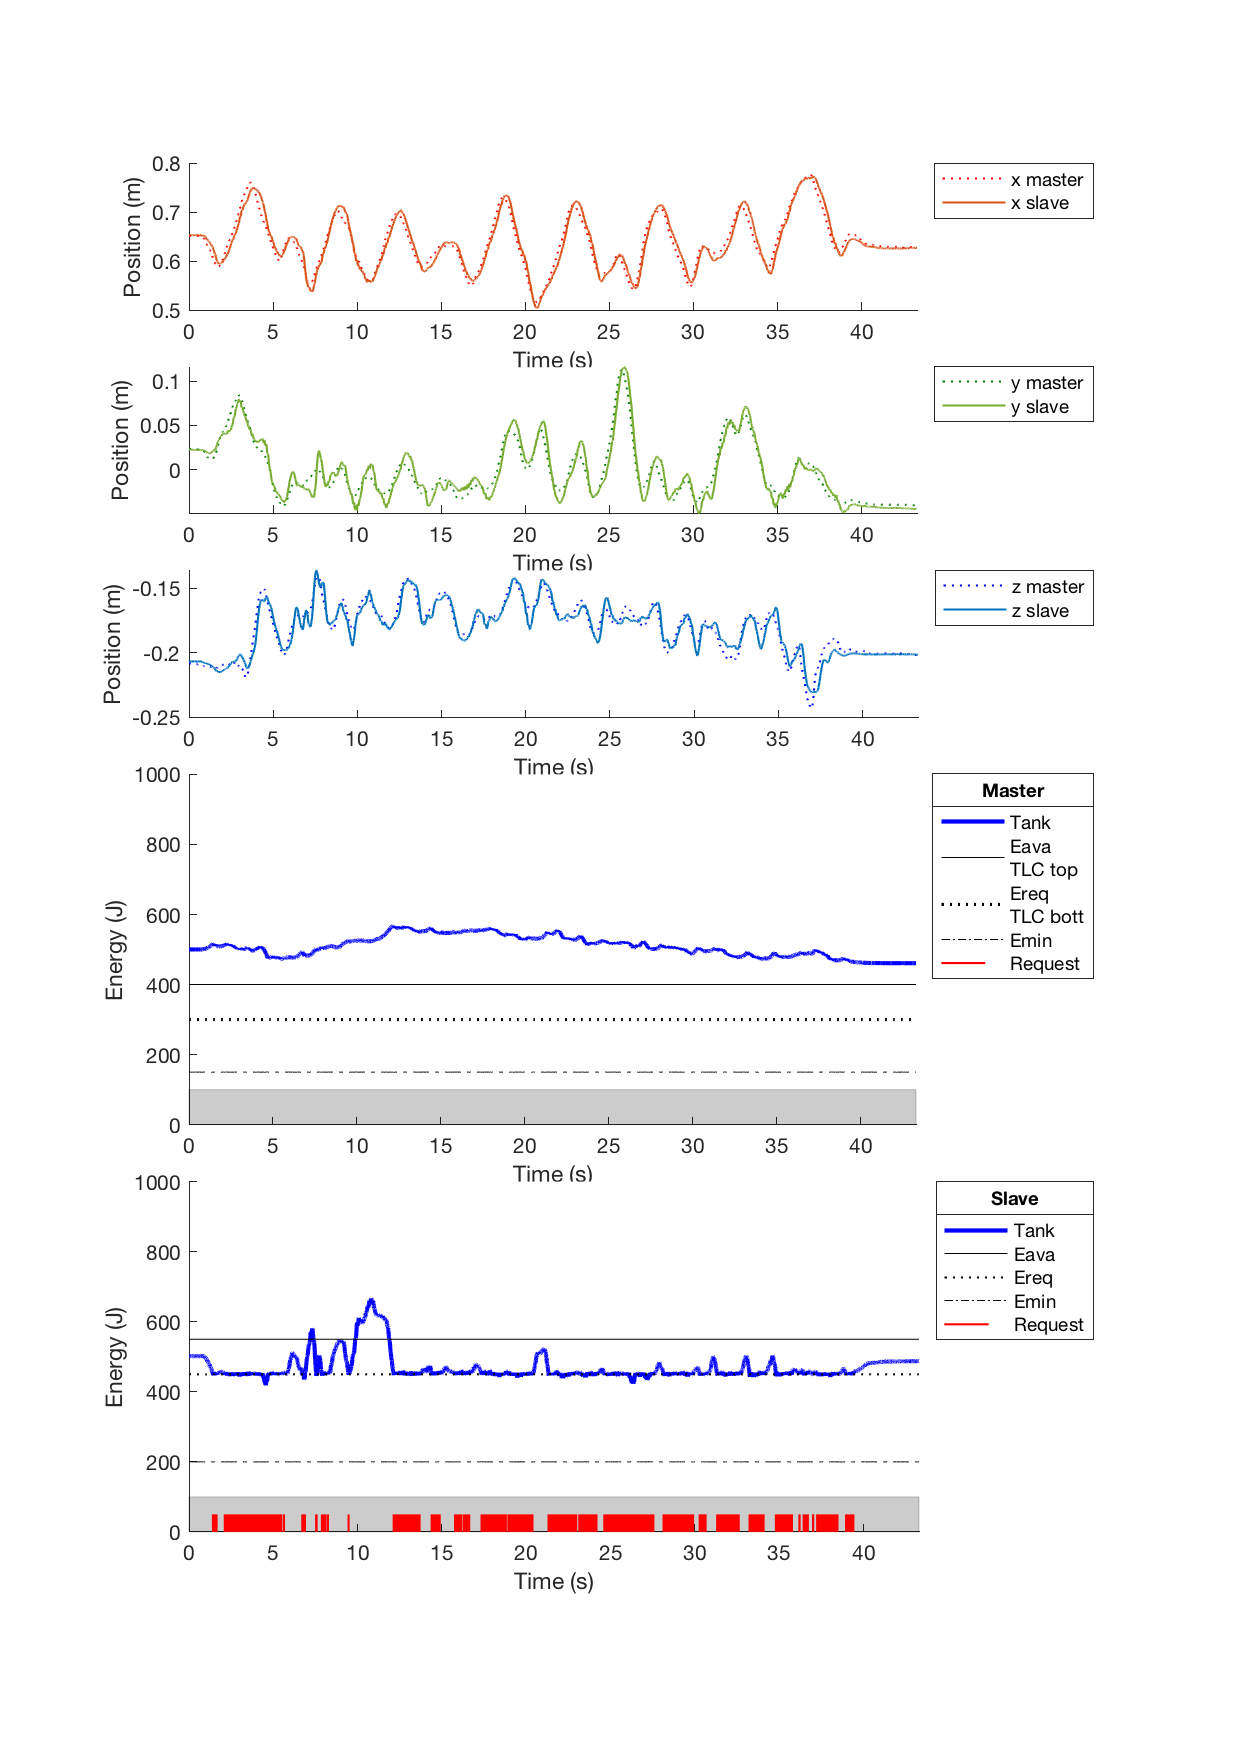
\includegraphics[width=\textwidth, keepaspectratio]{plots/ppFree/Position.pdf}
		\caption{Position tracking in free motion. P-P architecture without delay.}
		\label{graph:ppFree/Position}
	\end{figure}
\end{center}
\begin{center}
		\begin{figure}
		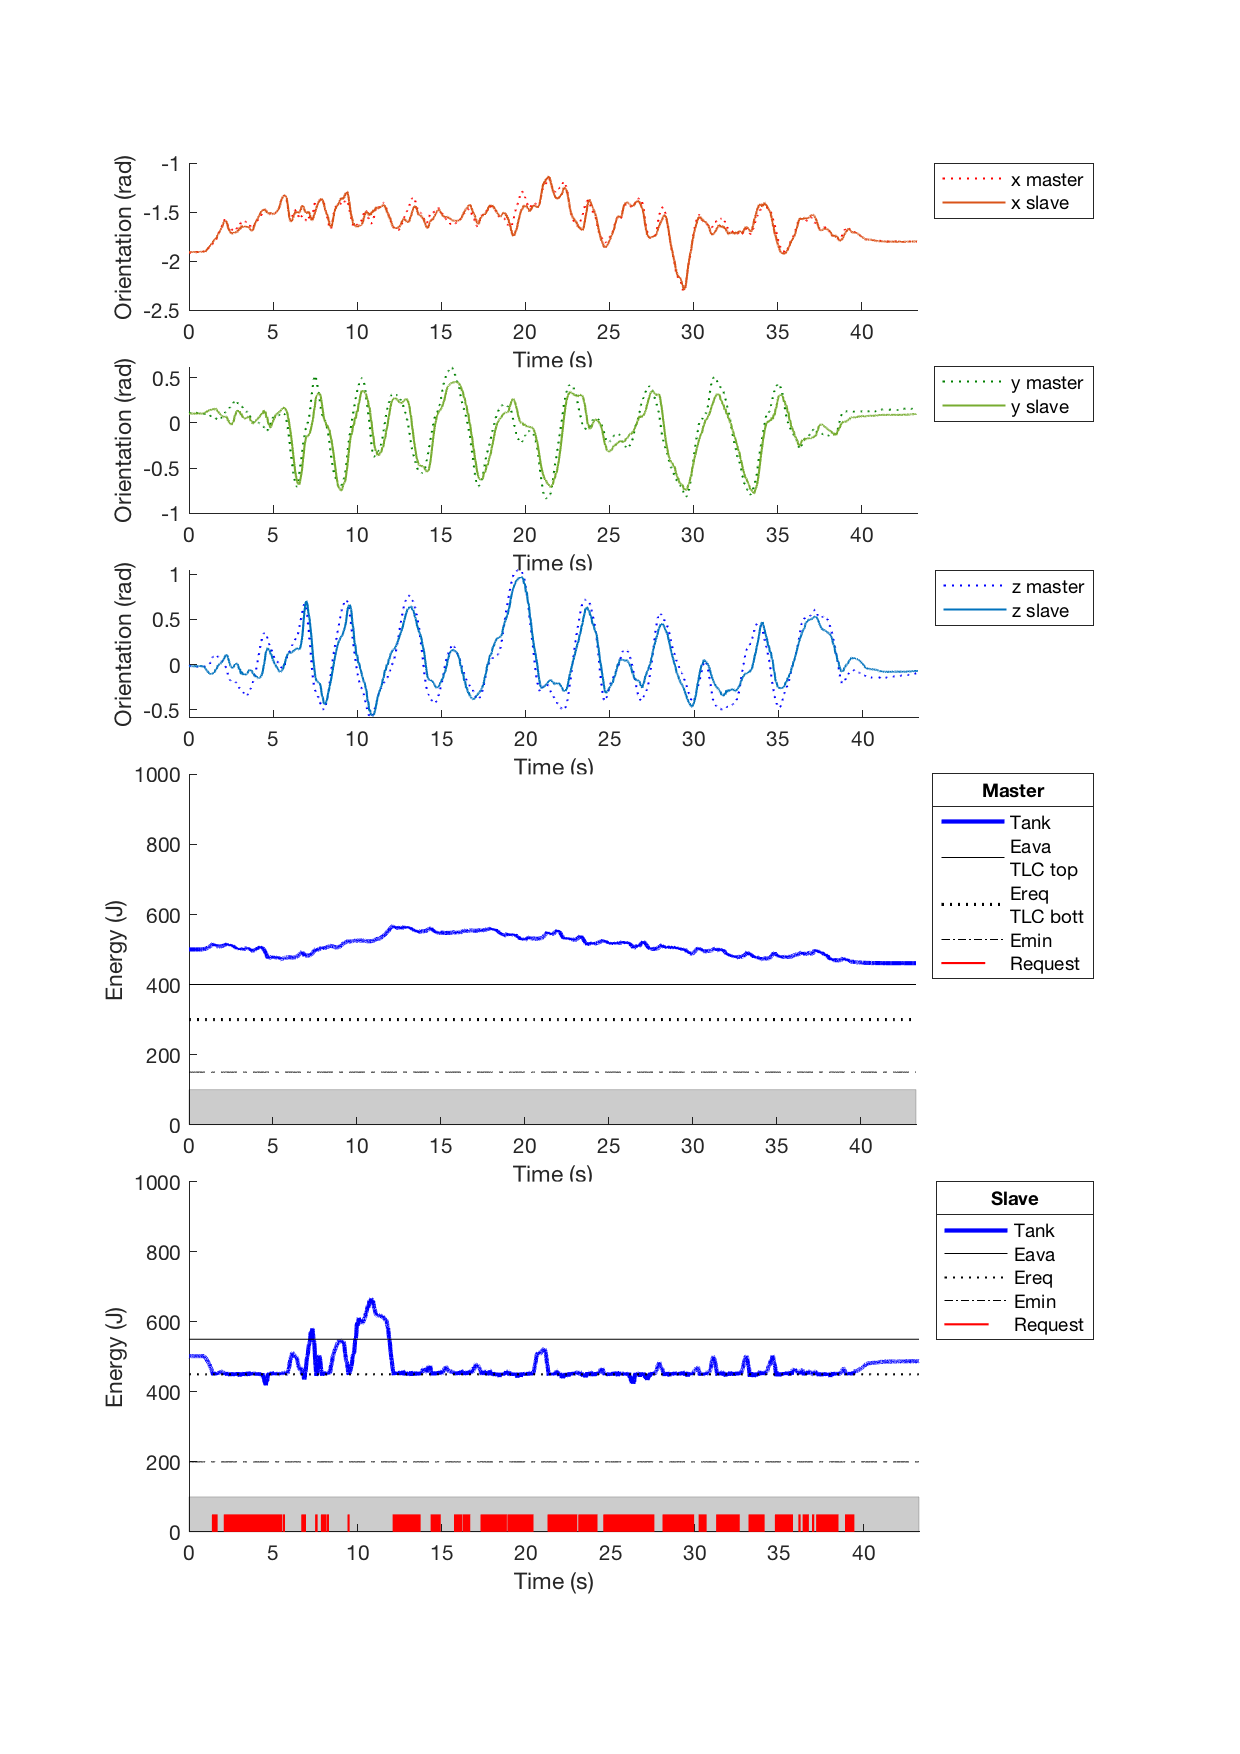
\includegraphics[width=\textwidth, keepaspectratio]{plots/ppFree/Orientation.pdf}
		\caption{Orientation tracking in free motion. P-P control architecture without delay.}
		\label{graph:ppFree/Orientation}
	\end{figure}
\end{center}
\begin{center}
	\begin{figure}
	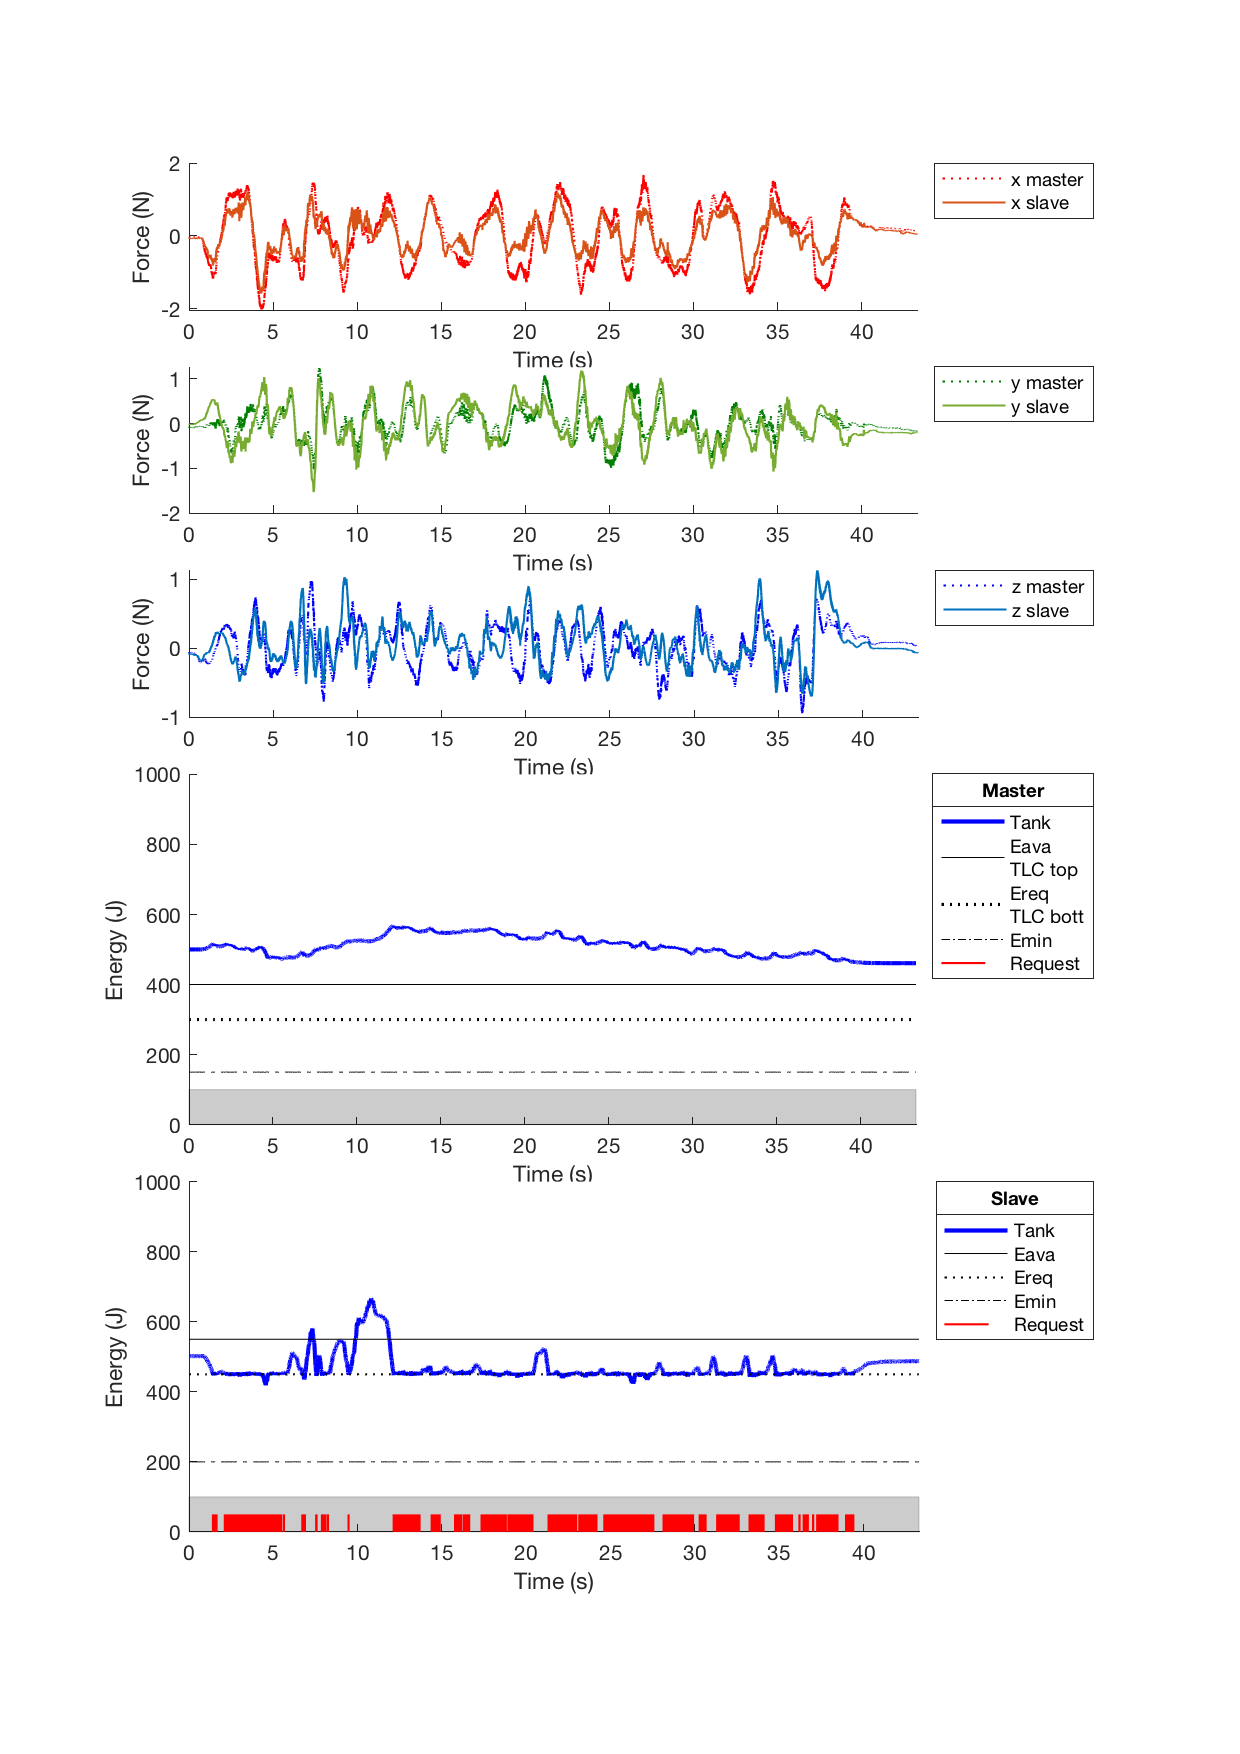
\includegraphics[width=\textwidth, keepaspectratio]{plots/ppFree/Force.pdf}
	\caption{Force tracking in free motion. P-P control architecture without delay.}
	\label{graph:ppFree/Force}
\end{figure}
\end{center}
\newpage
\subsubsection{Insertion with 90° approaching angle}\label{sec:insertion-with-90-approaching-angle1}
In this test  (\figurename s{ \ref{graph:pp90/Position} to \ref{graph:pp90/Force}}) the first two punctures have been done within the \textit{Pilot Mode}, described in Section \ref{PP_architecture}, and the other two with the standard controller.\\
With this switch of controller we want to show the benefit of the \textit{Pilot Mode} for the insertion procedure.
The change of controller at time 38.8s is highlighted by a vertical line.

The motion along of the $x-y$ reference from the master in \figurename{ \ref{graph:pp90/Position}} is due to it's not perfect 90° orientation with respect to the plane when starting the test (the desired motion is along the $z$ axis, orthogonal to the tissue or the $x-y$ plane). This happens because, without actuation on the three orientation DoF on the master, it is challenging to keep the correct starting position and orientation by hand.

The \textit{pilot mode} provides a feasible insertion trajectory thus, when we perform an insertion with this feature enabled, the energy in the system is well balanced.
When the insertion is performed with the standard controller, we experienced some issues due to the lack of feedback on the orientation.
In fact on the orientation the teleoperation is unilateral: when the needle sinks inside the tissue a small change in the tip orientation involves a large movements at the needle base and along its shaft.\\
When inside the tissue, the needle shaft is constrained in its movements by the tissue itself. If we change the orientation while performing the puncturing, the tissue exert a reaction force on the needle shaft that we are unable to provide to the operator.\\
We see the side effect of this force as an increased energy consumption while performing the task.
When the energy consumption becomes too high, the value chosen for energy scale factor ($\alpha/\gamma$) cannot balance the increased energy needs from the slave.

The final tracking error along $z$ between the master and the slave is due to the fact that the needle base reaches the top of the tissue. This is a common factor of all the test.
%since the effects from the inertia of the slave overcome the contact feedback, due to the displacement between master and slave, provided by the architecture.
\begin{center}
	\begin{figure}
		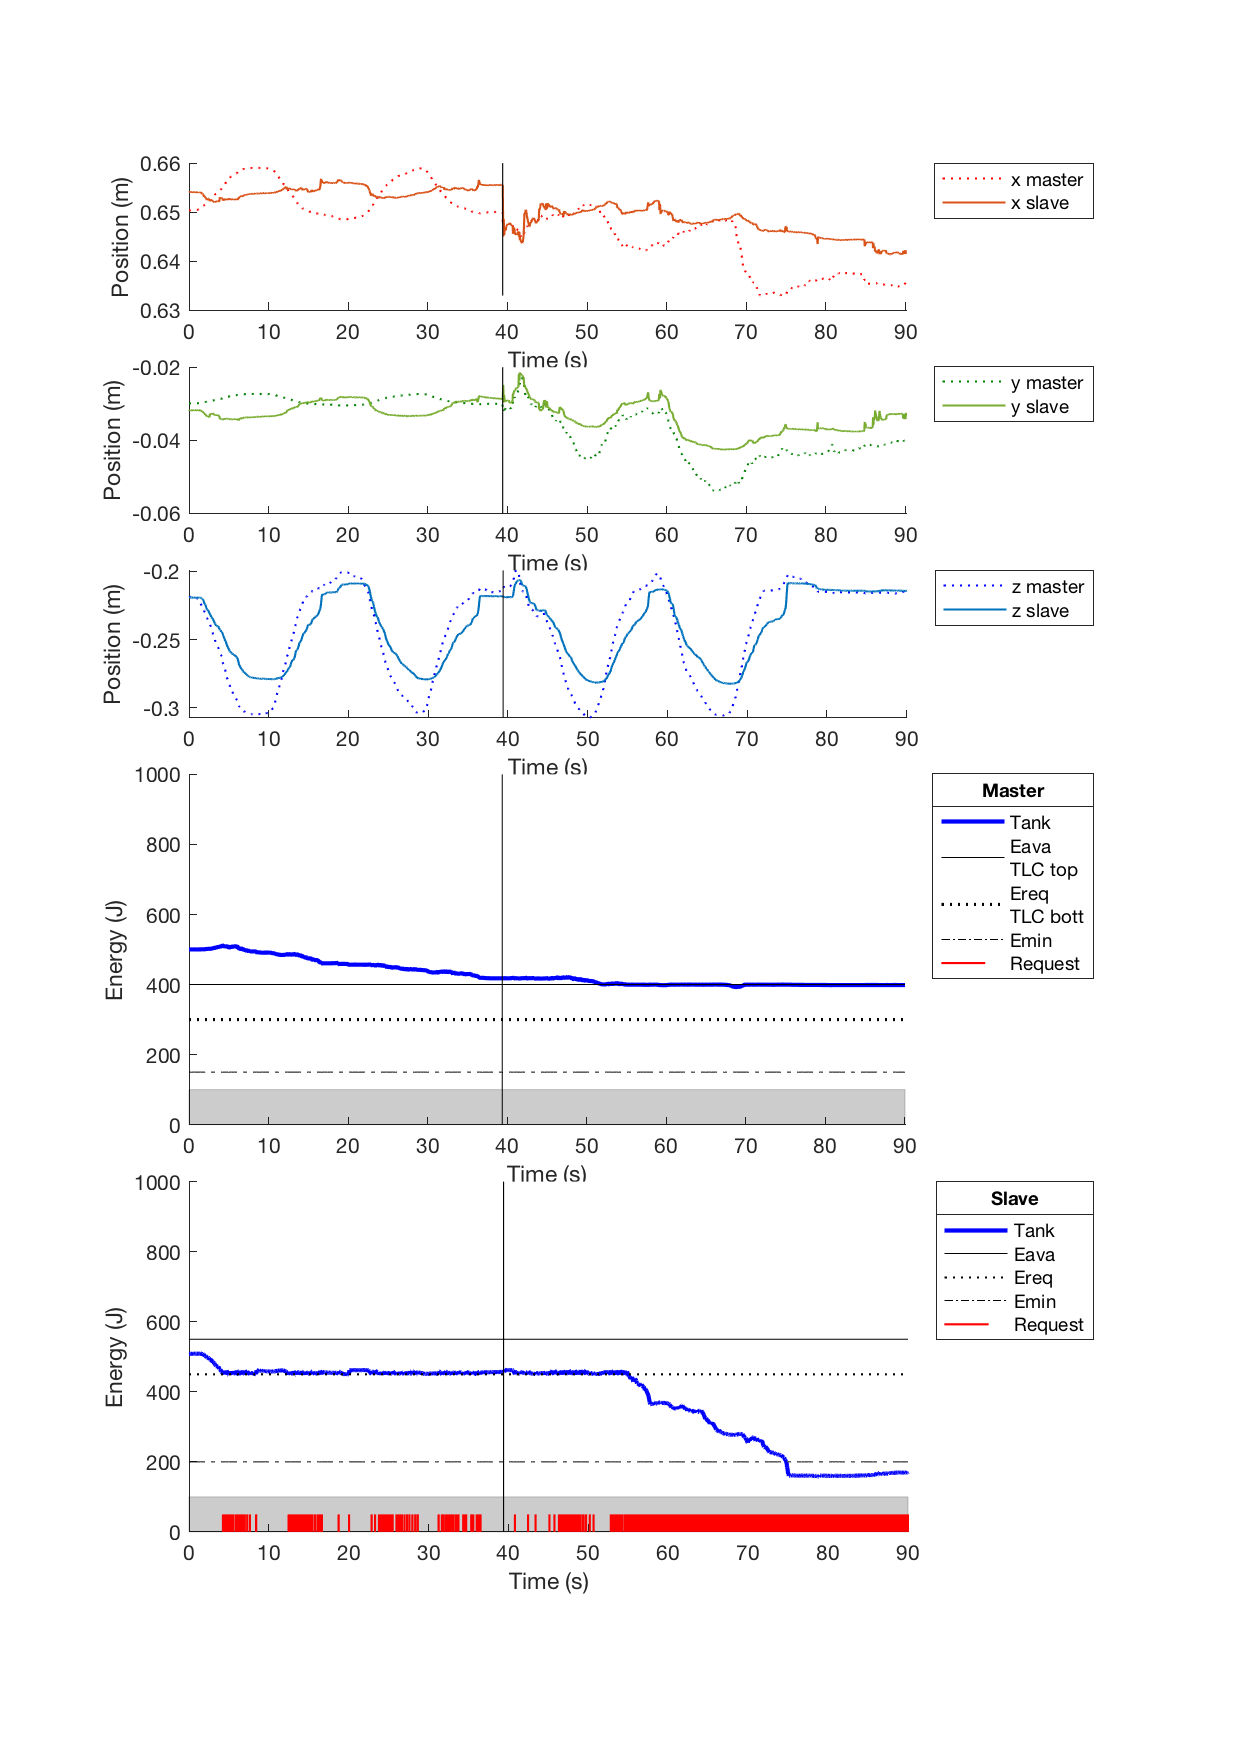
\includegraphics[width=\textwidth, keepaspectratio]{plots/pp90/Position.pdf}
		\caption{Position tracking with 90° insertion approach. P-P control architecture without delay.}
		\label{graph:pp90/Position}
	\end{figure}
\end{center}
\begin{center}
	\begin{figure}
		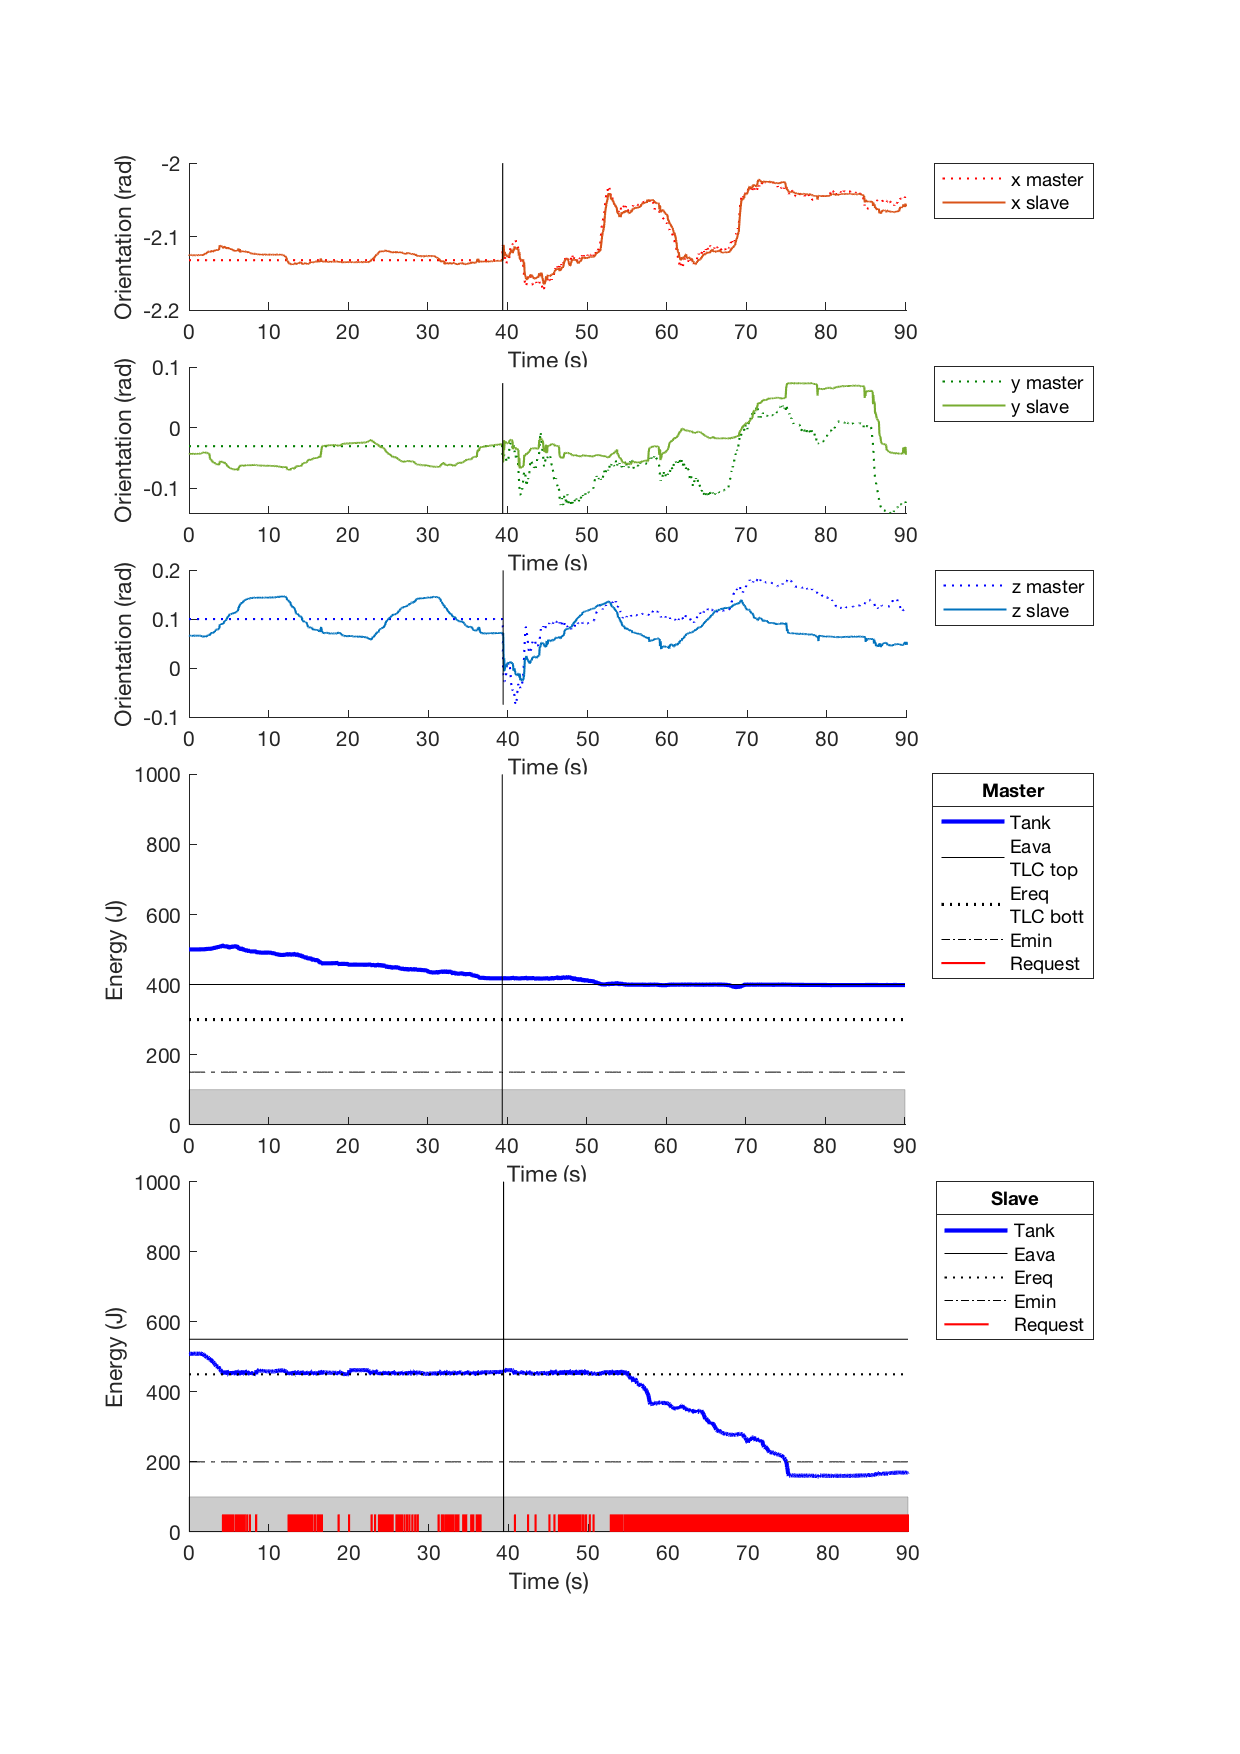
\includegraphics[width=\textwidth, keepaspectratio]{plots/pp90/Orientation.pdf}
		\caption{Orientation tracking with 90° insertion approach. P-P control architecture without delay.}
		\label{graph:pp90/Orientation}
	\end{figure}
\end{center}
\begin{center}
	\begin{figure}
		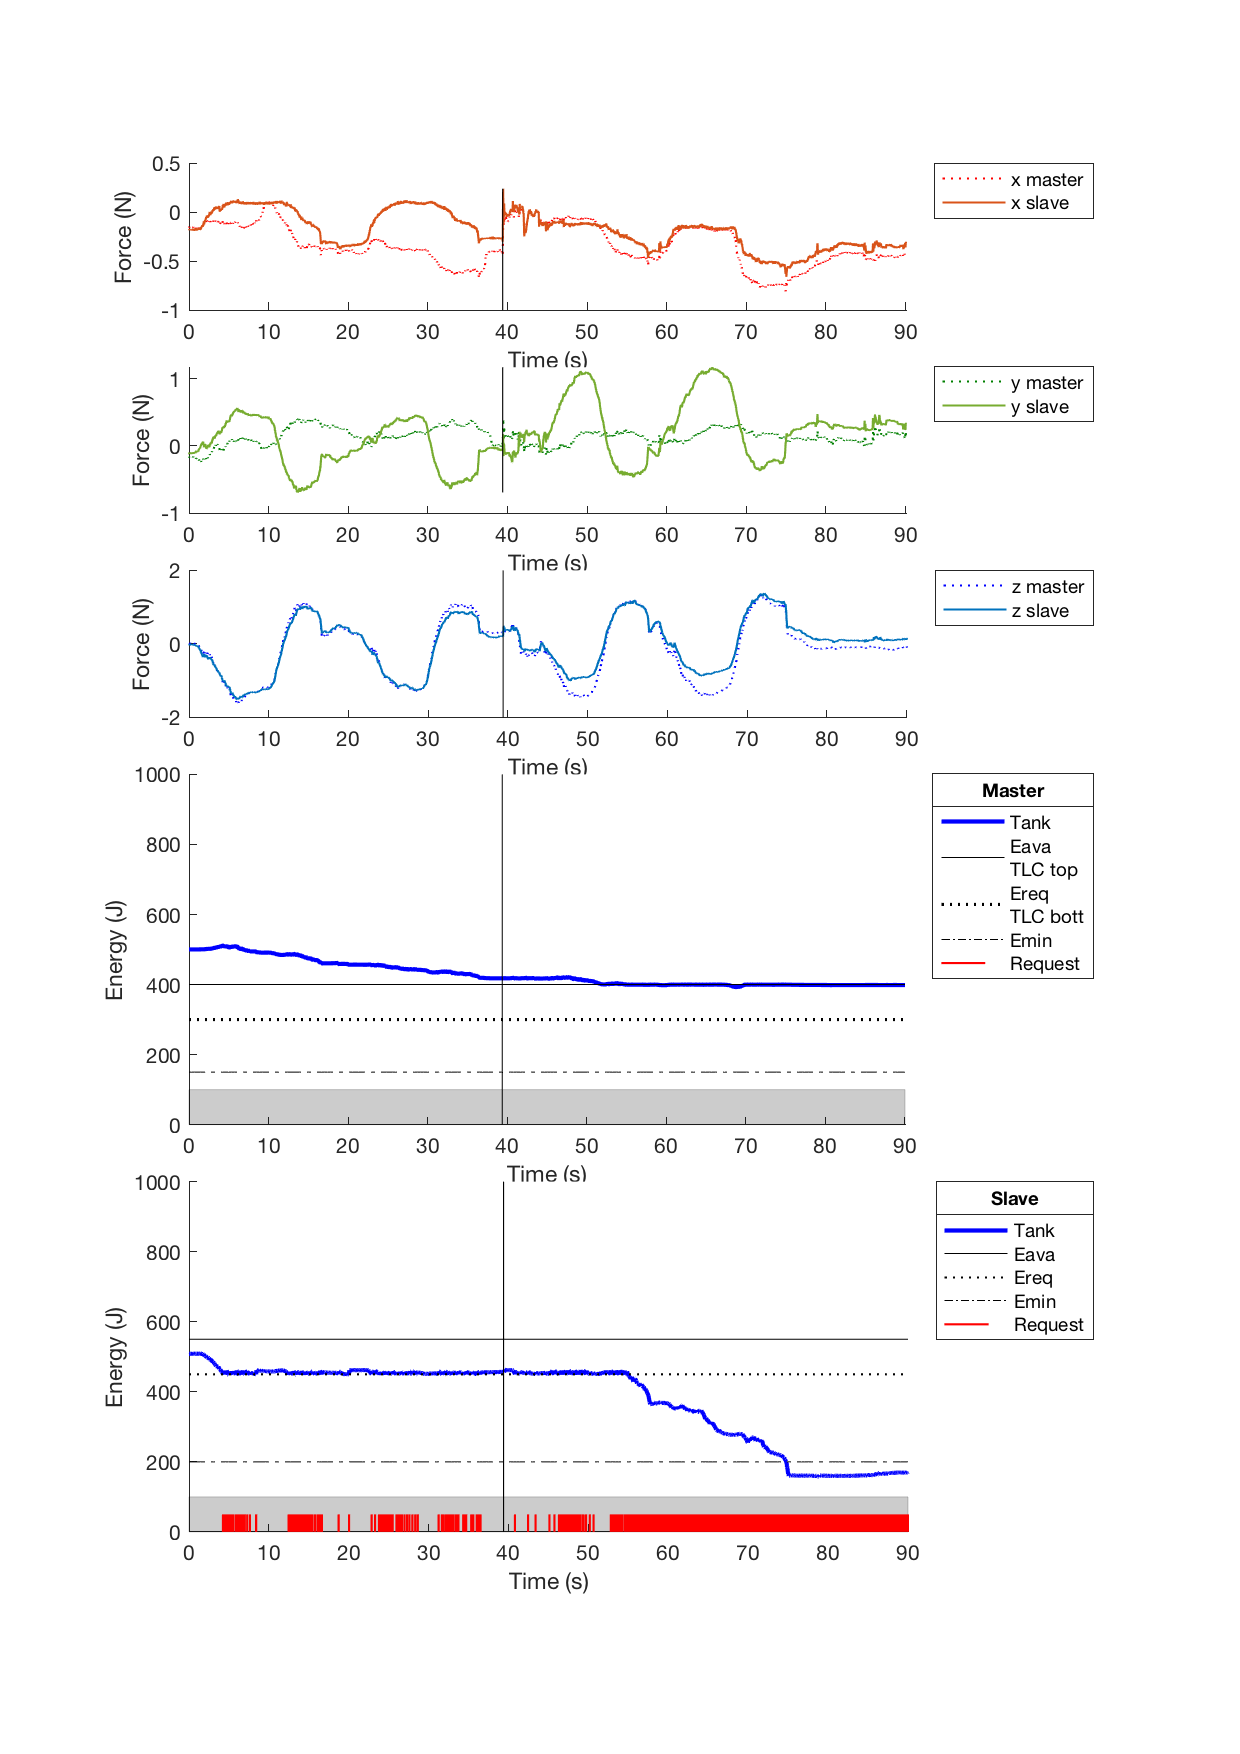
\includegraphics[width=\textwidth, keepaspectratio]{plots/pp90/Force.pdf}
		\caption{Force tracking with 90° insertion approach. P-P control architecture without delay.}
		\label{graph:pp90/Force}
	\end{figure}
\end{center}
\newpage
\subsubsection{Insertion with 45° approaching angle}
In this test (\figurename{ \ref{graph:pp45/Position} to \ref{graph:pp45/Force}}) the first two punctures have been executed within the \textit{Pilot Mode} and the other two with the standard controller.
The change of controller at time 30.4s is highlighted by a vertical line.
The system is more stable when the insertion is artificially controlled, thus the inserting direction causes the tissue to exert a greater force on the $(x-y)$ needle axes. This means that the slave requires more energy than in the previous experiment.
When the operator is free to move, the slave reaches the minimum value of energy that the tank must keep at time 53s, thus it does not apply the controller commands.
\begin{center}
	\begin{figure}
		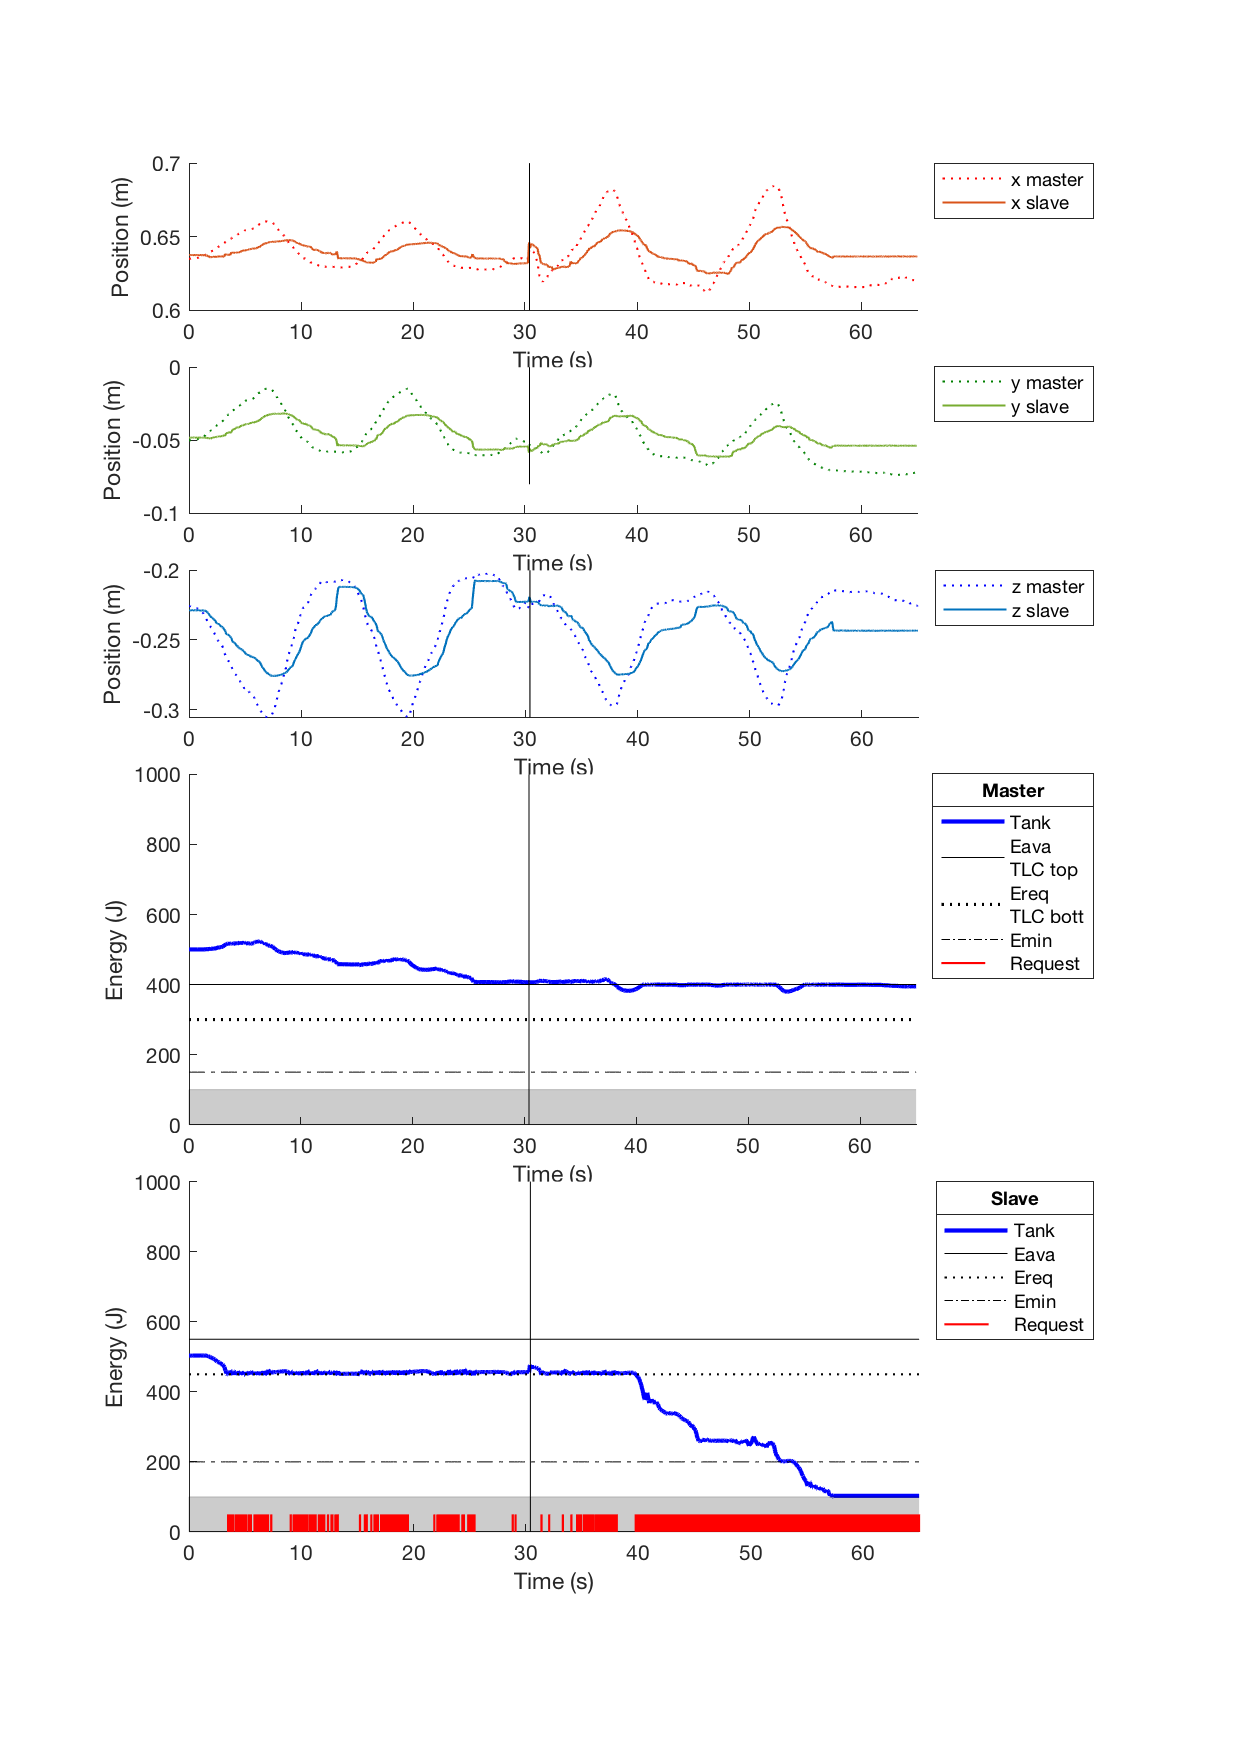
\includegraphics[width=\textwidth, keepaspectratio]{plots/pp45/Position.pdf}
		\caption{Position tracking with 45° insertion approach. P-P control architecture without delay.}
		\label{graph:pp45/Position}
	\end{figure}
\end{center}
\begin{center}
	\begin{figure}
		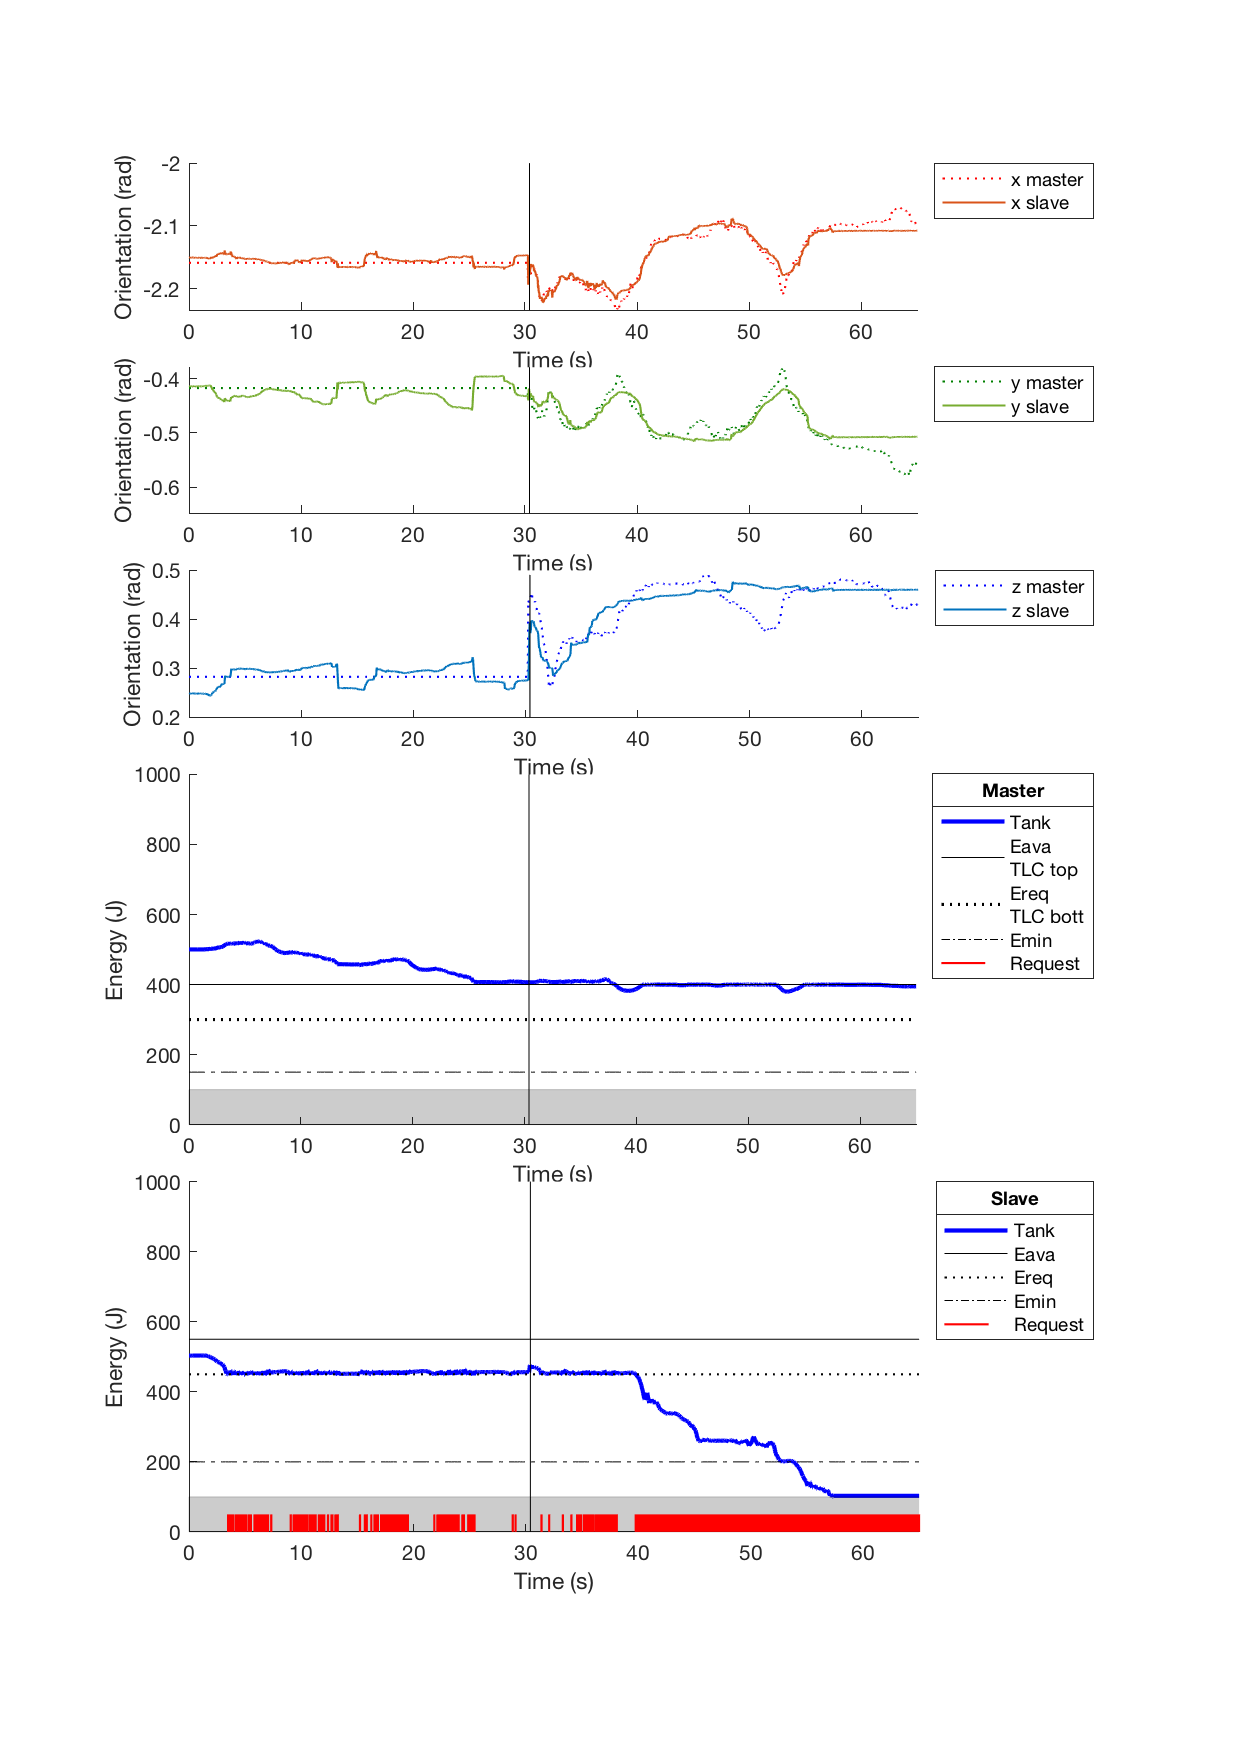
\includegraphics[width=\textwidth, keepaspectratio]{plots/pp45/Orientation.pdf}
		\caption{Orientation tracking with 45° insertion approach. P-P control architecture without delay.}
		\label{graph:pp45/Orientation}
	\end{figure}
\end{center}
\begin{center}
	\begin{figure}
		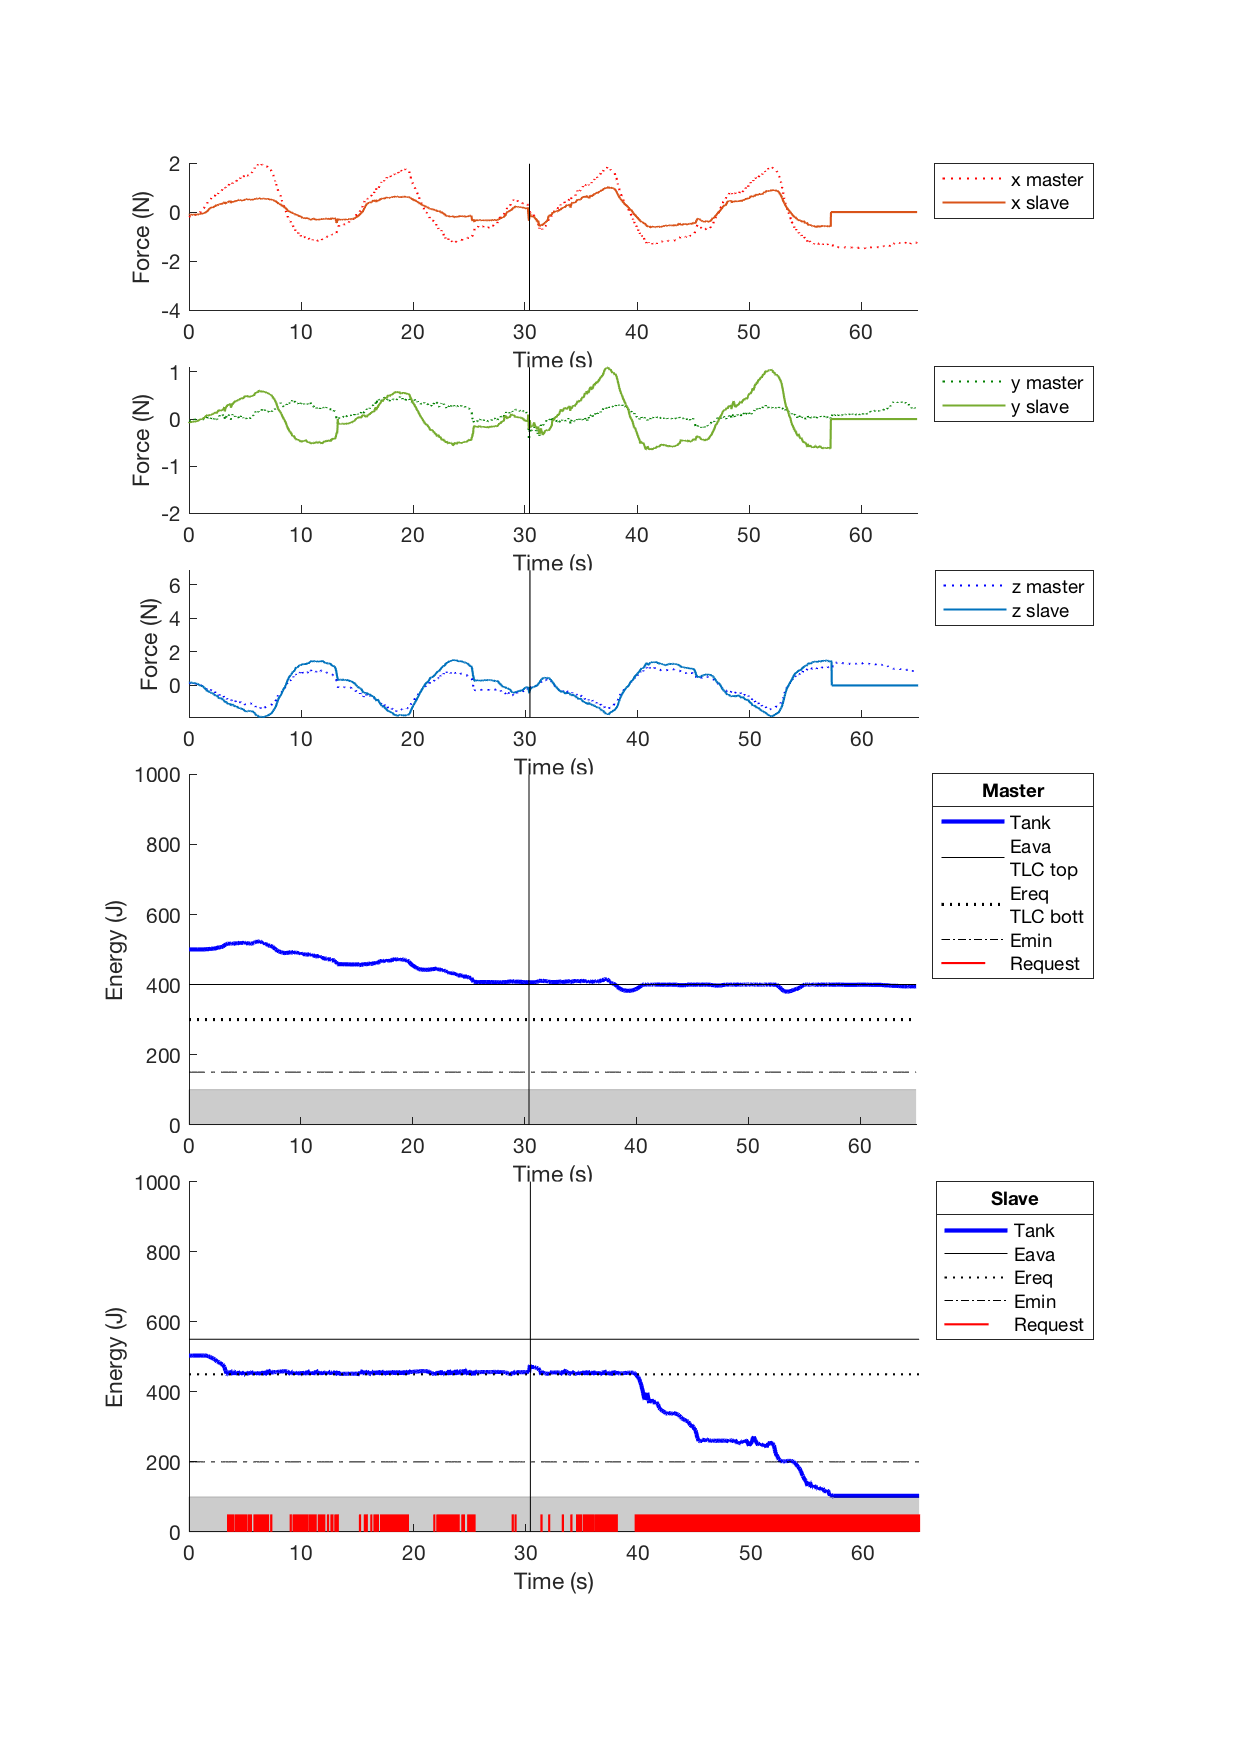
\includegraphics[width=\textwidth, keepaspectratio]{plots/pp45/Force.pdf}
		\caption{Force tracking with 45° insertion approach. P-P control architecture without delay.}
		\label{graph:pp45/Force}
	\end{figure}
\end{center}
\newpage
\subsection{Constant Delay}
\subsubsection{Free motion}
The free motion tests have been repeated introducing a constant delay into the communication channel (\figurename s{ \ref{graph:ppFreeDelay/Position} to \ref{graph:ppFreeDelay/Force}}).
It's interesting looking at the energy level in the tanks. Due to the delay the position tracking error increases especially when there are changes in the motion direction. This is felt by the operator as a larger force to overcome. Thus the operators provides more energy to the system. In this free motion scenario the position changes quite fast, as shown in \figurename{ \ref{graph:ppFreeDelay/Position}}, thus the damping coefficient clearly shows its effects at the master side in \figurename{ \ref{graph:ppFreeDelay/Force}}.
The energy level in the slave tank increases and decreases really fast. This is due to the delay: in fact the system not only sees the energy requests delayed in time but, when the tank that is performing the request reaches the desired level of energy stored inside it, a RTT is needed to stop the incoming energy flow.
\begin{center} 
	\begin{figure}
		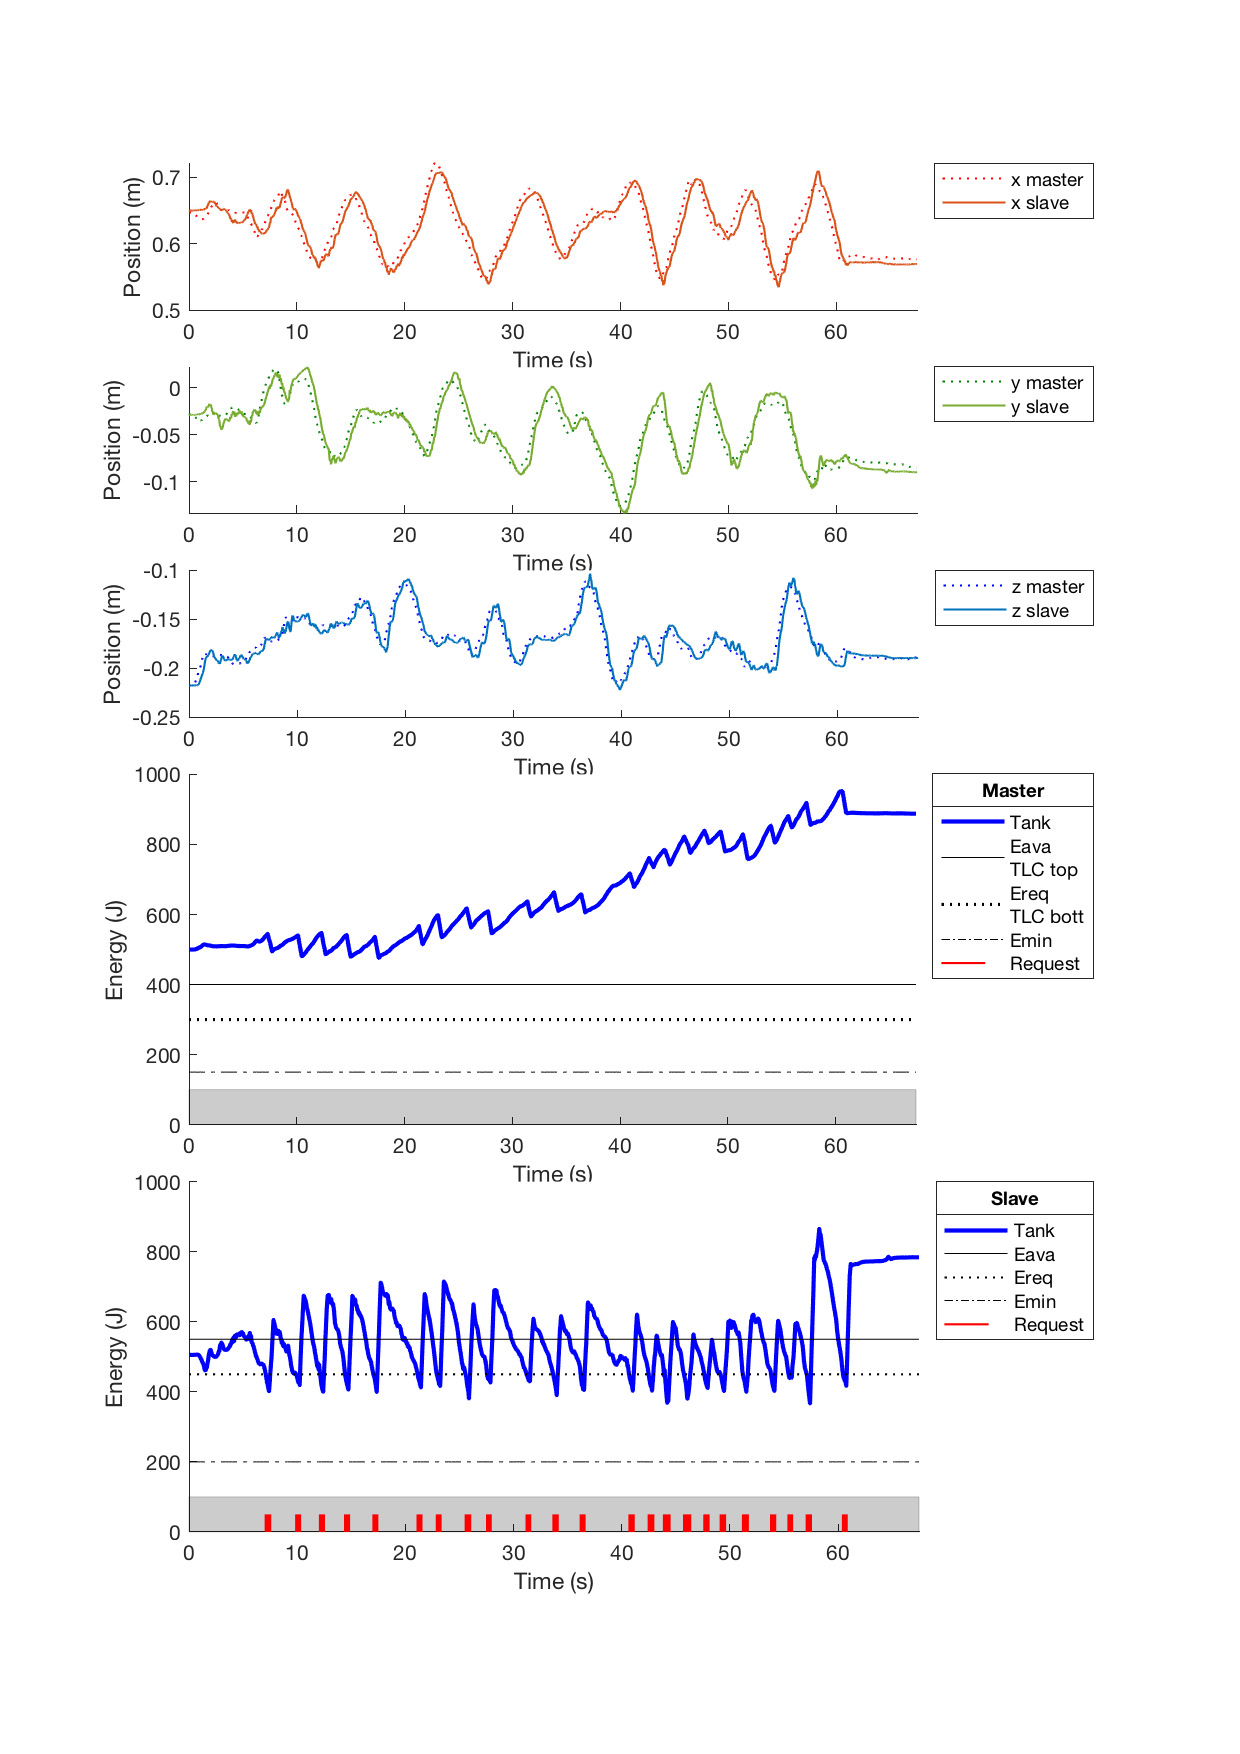
\includegraphics[width=\textwidth, keepaspectratio]{plots/ppDelay/Position.pdf}
		\caption{Position tracking in free motion. P-P control architecture with 0.2s RTT delay.}
		\label{graph:ppFreeDelay/Position}
	\end{figure}
\end{center}
\begin{center}
	\begin{figure}
		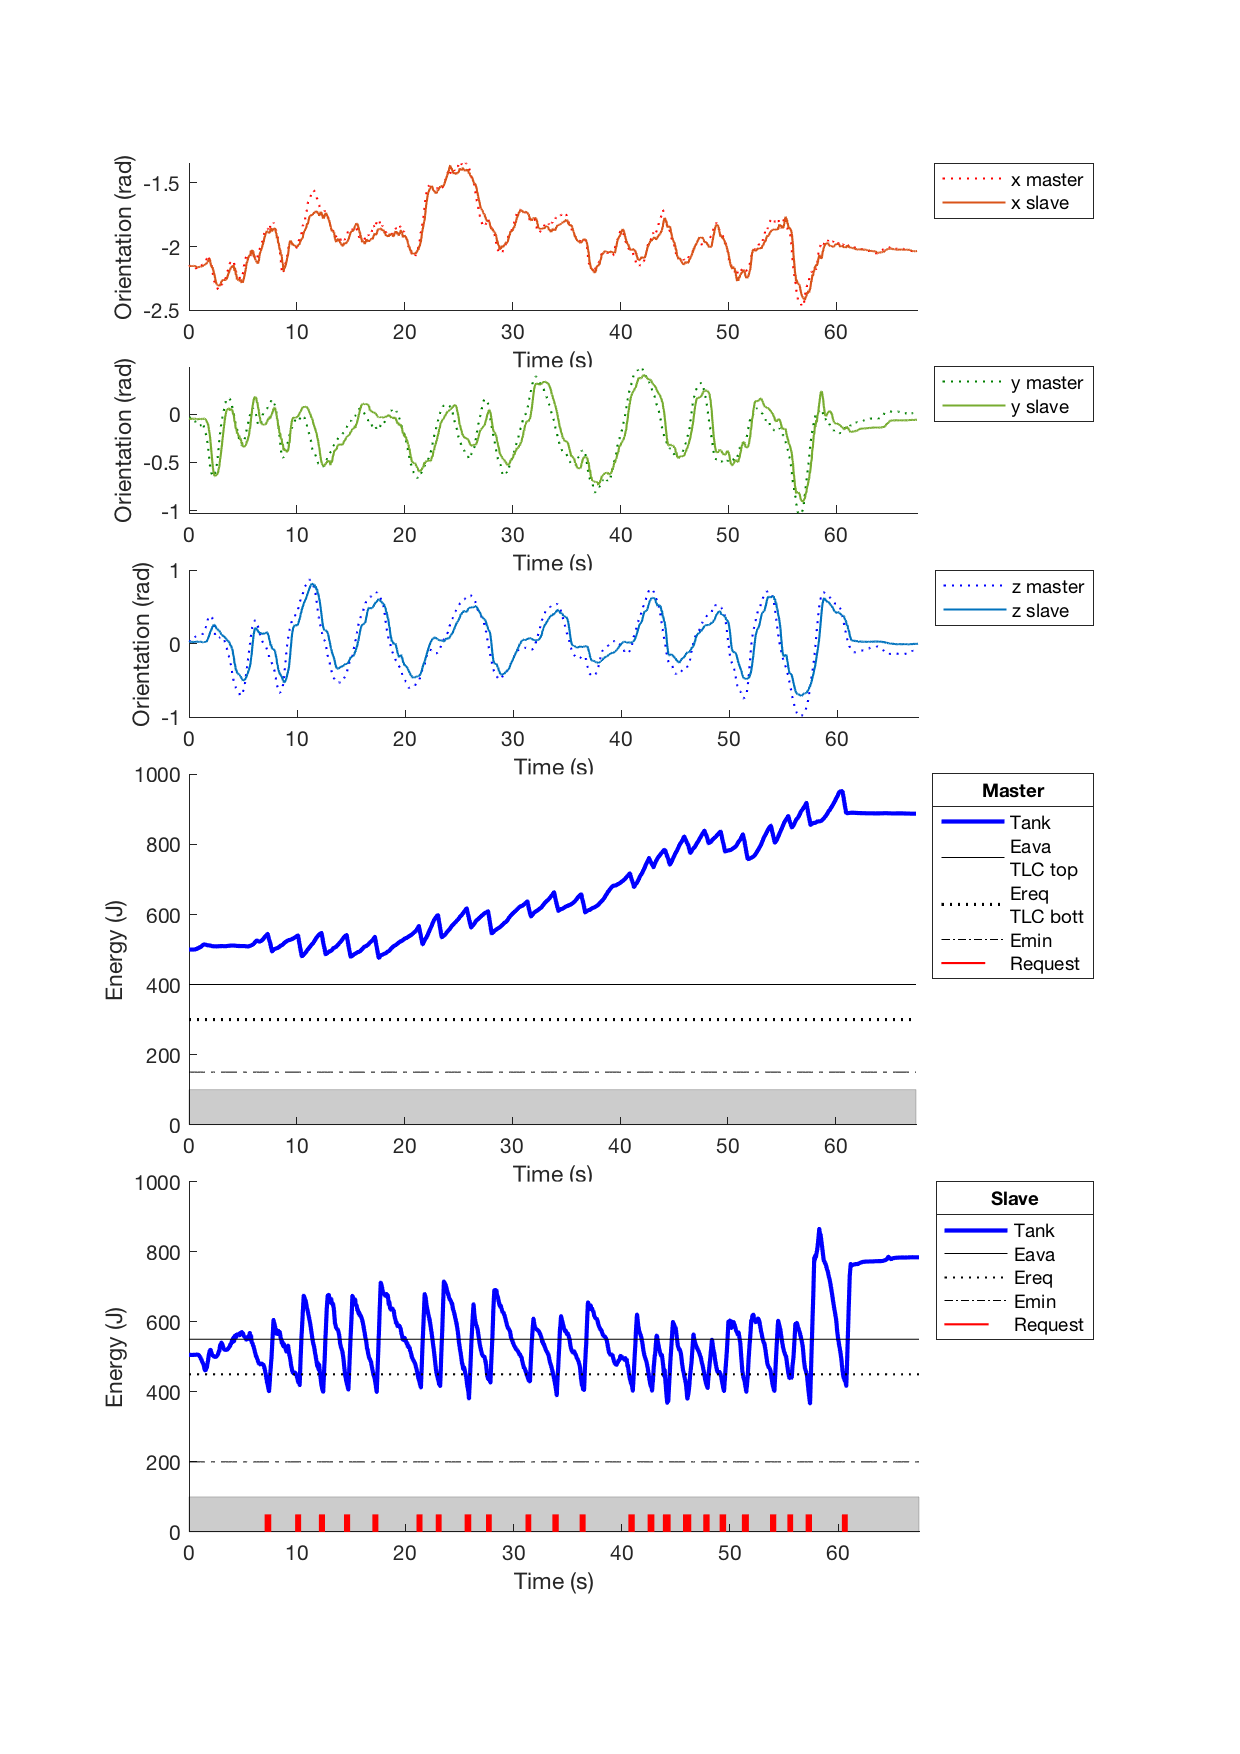
\includegraphics[width=\textwidth, keepaspectratio]{plots/ppDelay/Orientation.pdf}
		\caption{Orientation tracking in free motion. P-P control architecture with 0.2s RTT delay.}
		\label{graph:ppFreeDelay/Orientation}
	\end{figure}
\end{center}
\begin{center}
	\begin{figure}
		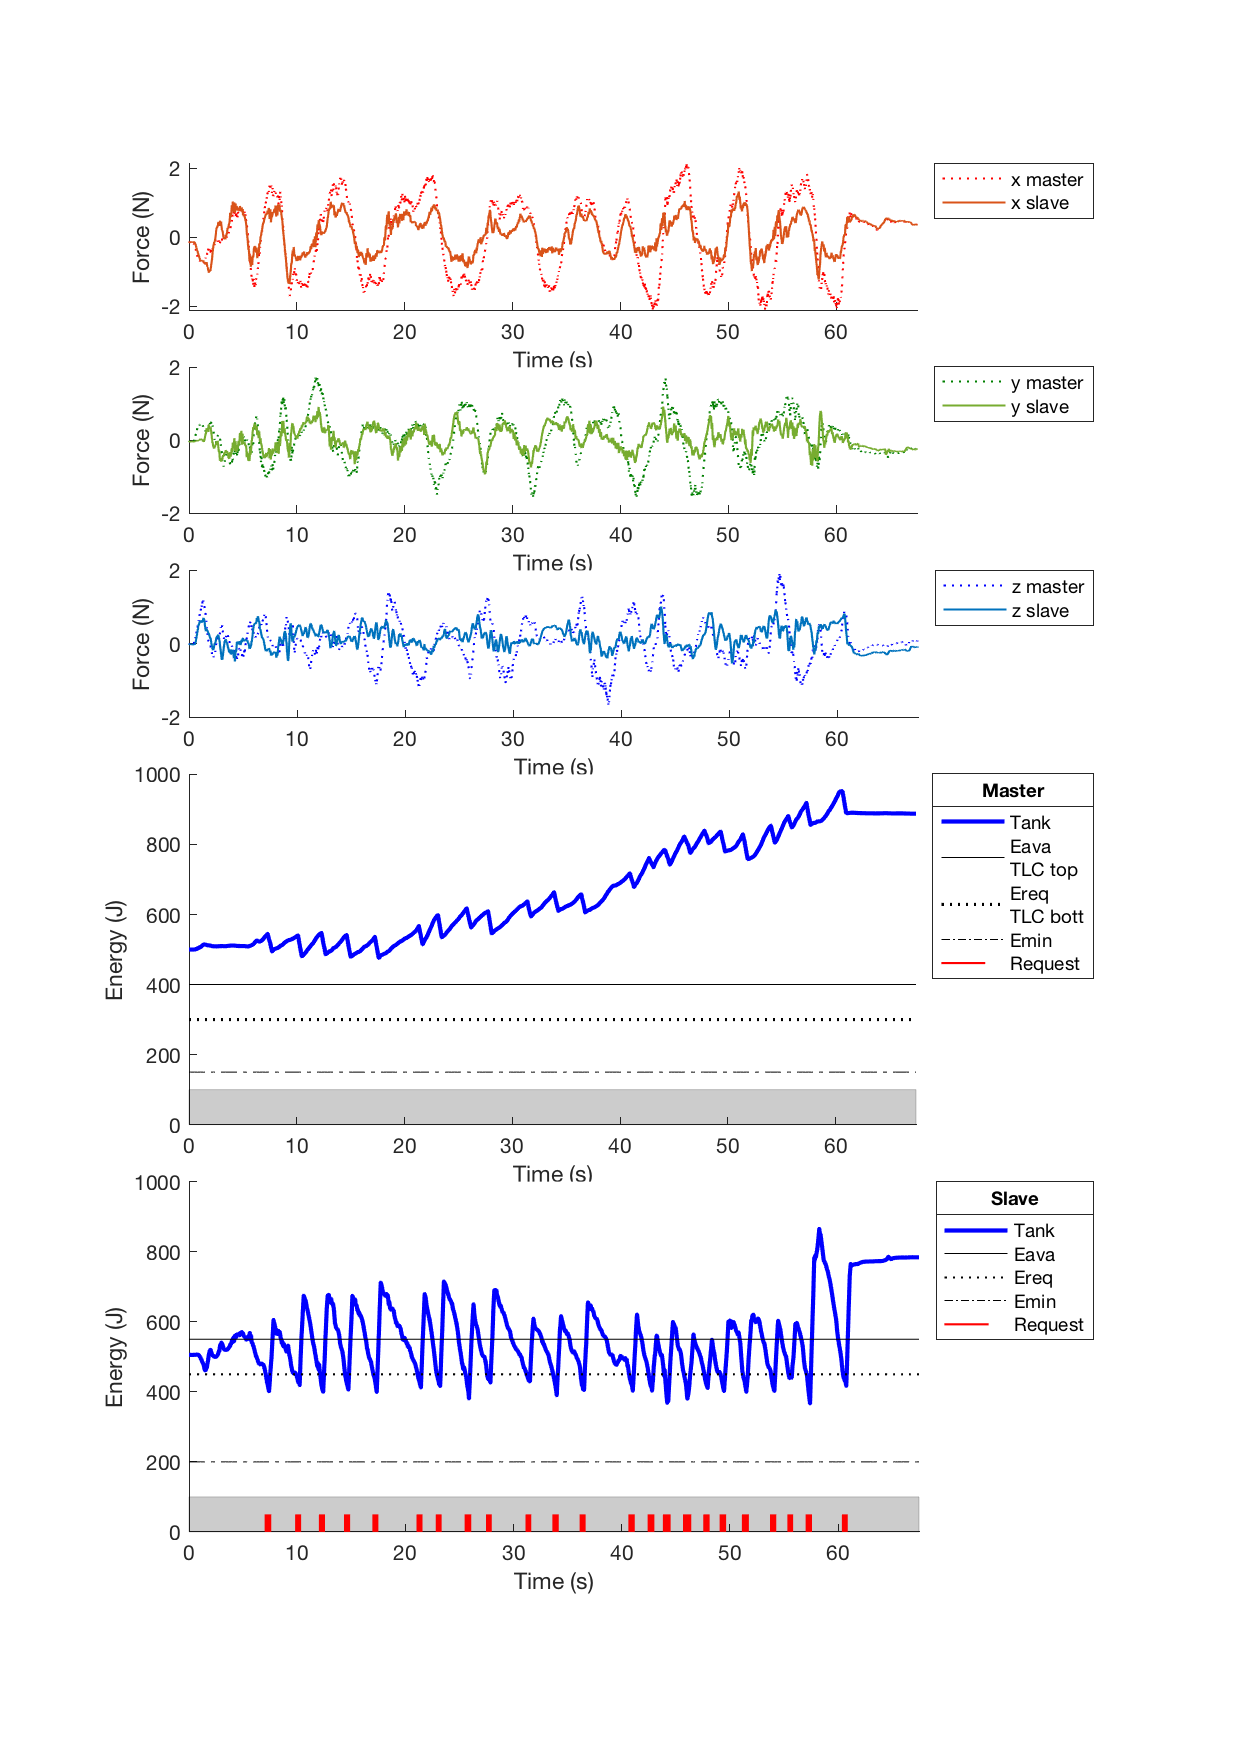
\includegraphics[width=\textwidth, keepaspectratio]{plots/ppDelay/Force.pdf}
		\caption{Force tracking in free motion. P-P control architecture with 0.2s RTT delay.}
		\label{graph:ppFreeDelay/Force}
	\end{figure}
\end{center}
\newpage
\subsubsection{Insertion 90° approaching angle}
In this test  (\figurename s{ \ref{graph:pp90Delay/Position} to \ref{graph:pp90Delay/Force}}) the first two punctures have been done within the \textit{Pilot Mode} and the other two with the standard controller.
The change of controller at time 38.8s is highlighted by a vertical line.
The behaviour of the position and orientation tracking is likely the same as in the no delayed version of the experiment. We can see again a non perfect initial positioning at the master side that causes the unexpected command along the $x-y$ axis.
The energy balance is preserved while using the \textit{Pilot Mode} as discussed in Section \ref{sec:insertion-with-90-approaching-angle1}.

Regards the tank level, we can se the behaviour discussed in the free motion with delay test.
The energy level in the slave tank increases and decreases really fast. This behaviour is due to the delay and to the RTT needed to start/stop the incoming energy flow.
When there is not enough energy at the master side to fulfil the slave requirements the behaviour is the same as the undelayed test.

The difference between the force behaviour in $x$ between master and slave that we can see in \figurename{ \ref{graph:pp90Delay/Force}}  is due to the fact that the operator is forcing the position commanded by the \textit{Pilot controller}. The master controller tries to push the operator into the right $x$ position.
\begin{center}
	\begin{figure}
		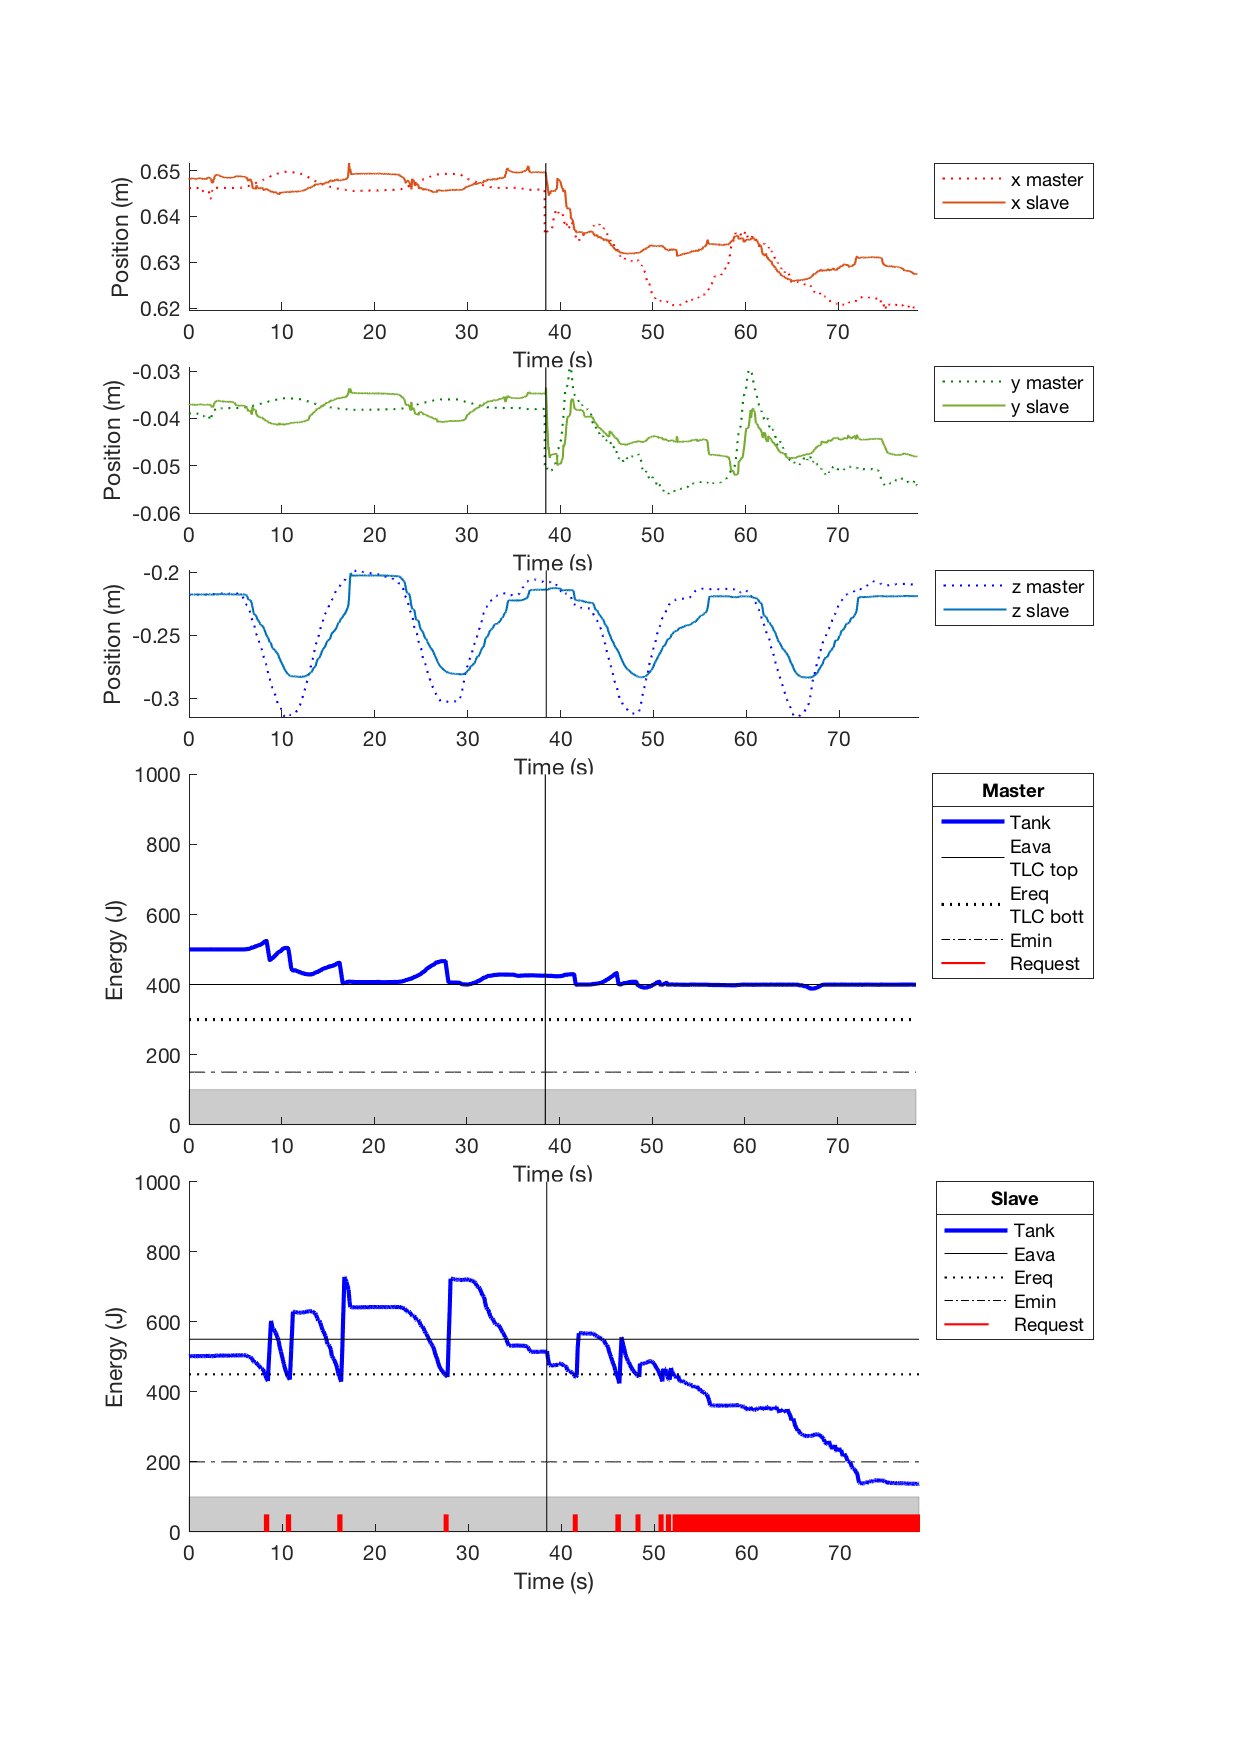
\includegraphics[width=\textwidth, keepaspectratio]{plots/pp90Delay/Position.pdf}
		\caption{Position tracking with 90° insertion approach. P-P control architecture with 0.2s RTT delay.}
		\label{graph:pp90Delay/Position}
	\end{figure}
\end{center}
\begin{center}
	\begin{figure}
		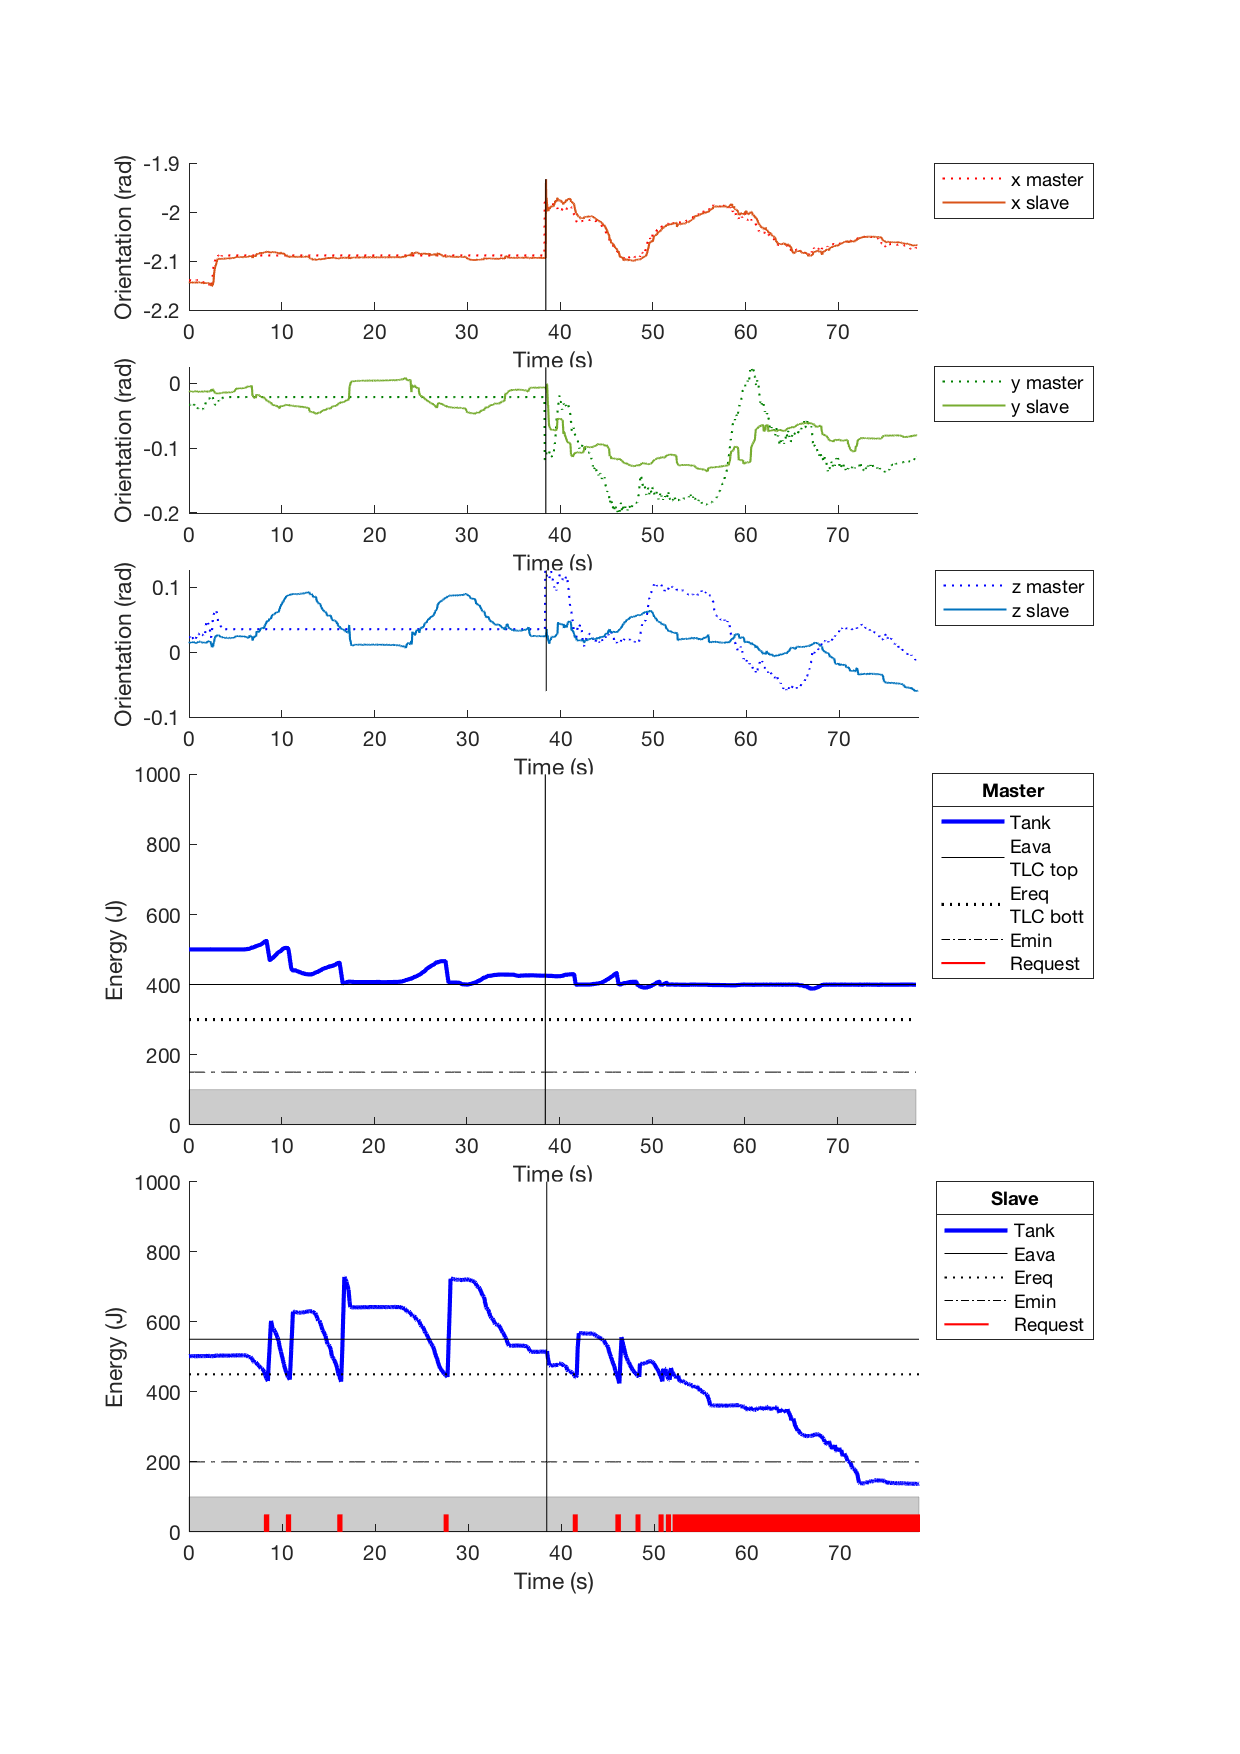
\includegraphics[width=\textwidth, keepaspectratio]{plots/pp90Delay/Orientation.pdf}
		\caption{Orientation tracking with 90° insertion approach. P-P control architecture with 0.2s RTT delay.}
		\label{graph:pp90Delay/Orientation}
	\end{figure}
\end{center}
\begin{center}
	\begin{figure}
		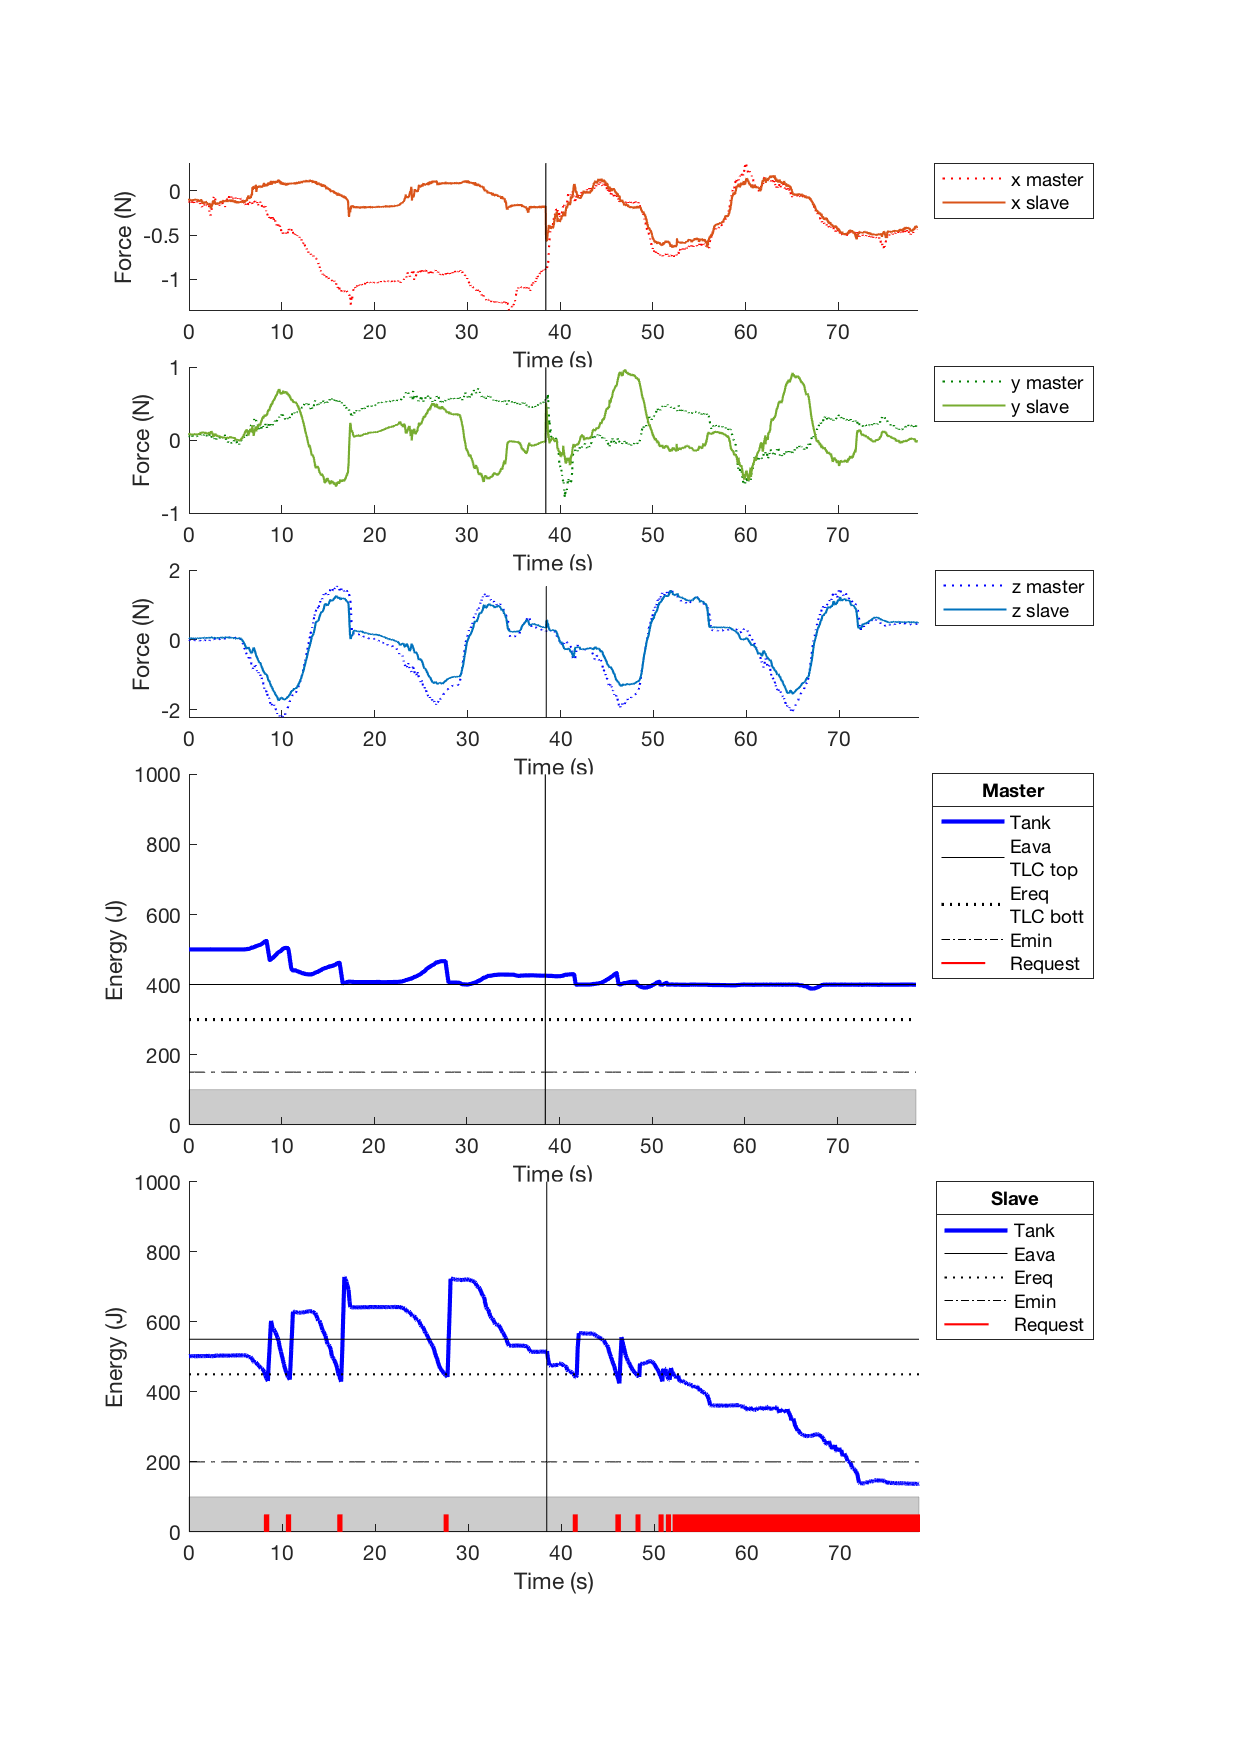
\includegraphics[width=\textwidth, keepaspectratio]{plots/pp90Delay/Force.pdf}
		\caption{Force tracking with 90° insertion approach. P-P control architecture with 0.2s RTT delay.}
		\label{graph:pp90Delay/Force}
	\end{figure}
\end{center}
\newpage
\subsubsection{Insertion with 45° approaching angle}
In this test (\figurename s{ \ref{graph:pp45Delay/Position} to \ref{graph:pp45Delay/Force}}) the first two punctures have been done within the \textit{Pilot Mode} and the other two with the standard controller.
The test is the delayed version of the one with 45° insertion previously commented.
The change of controller at time 40s is highlighted by a vertical line.
\begin{center}
	\begin{figure}
		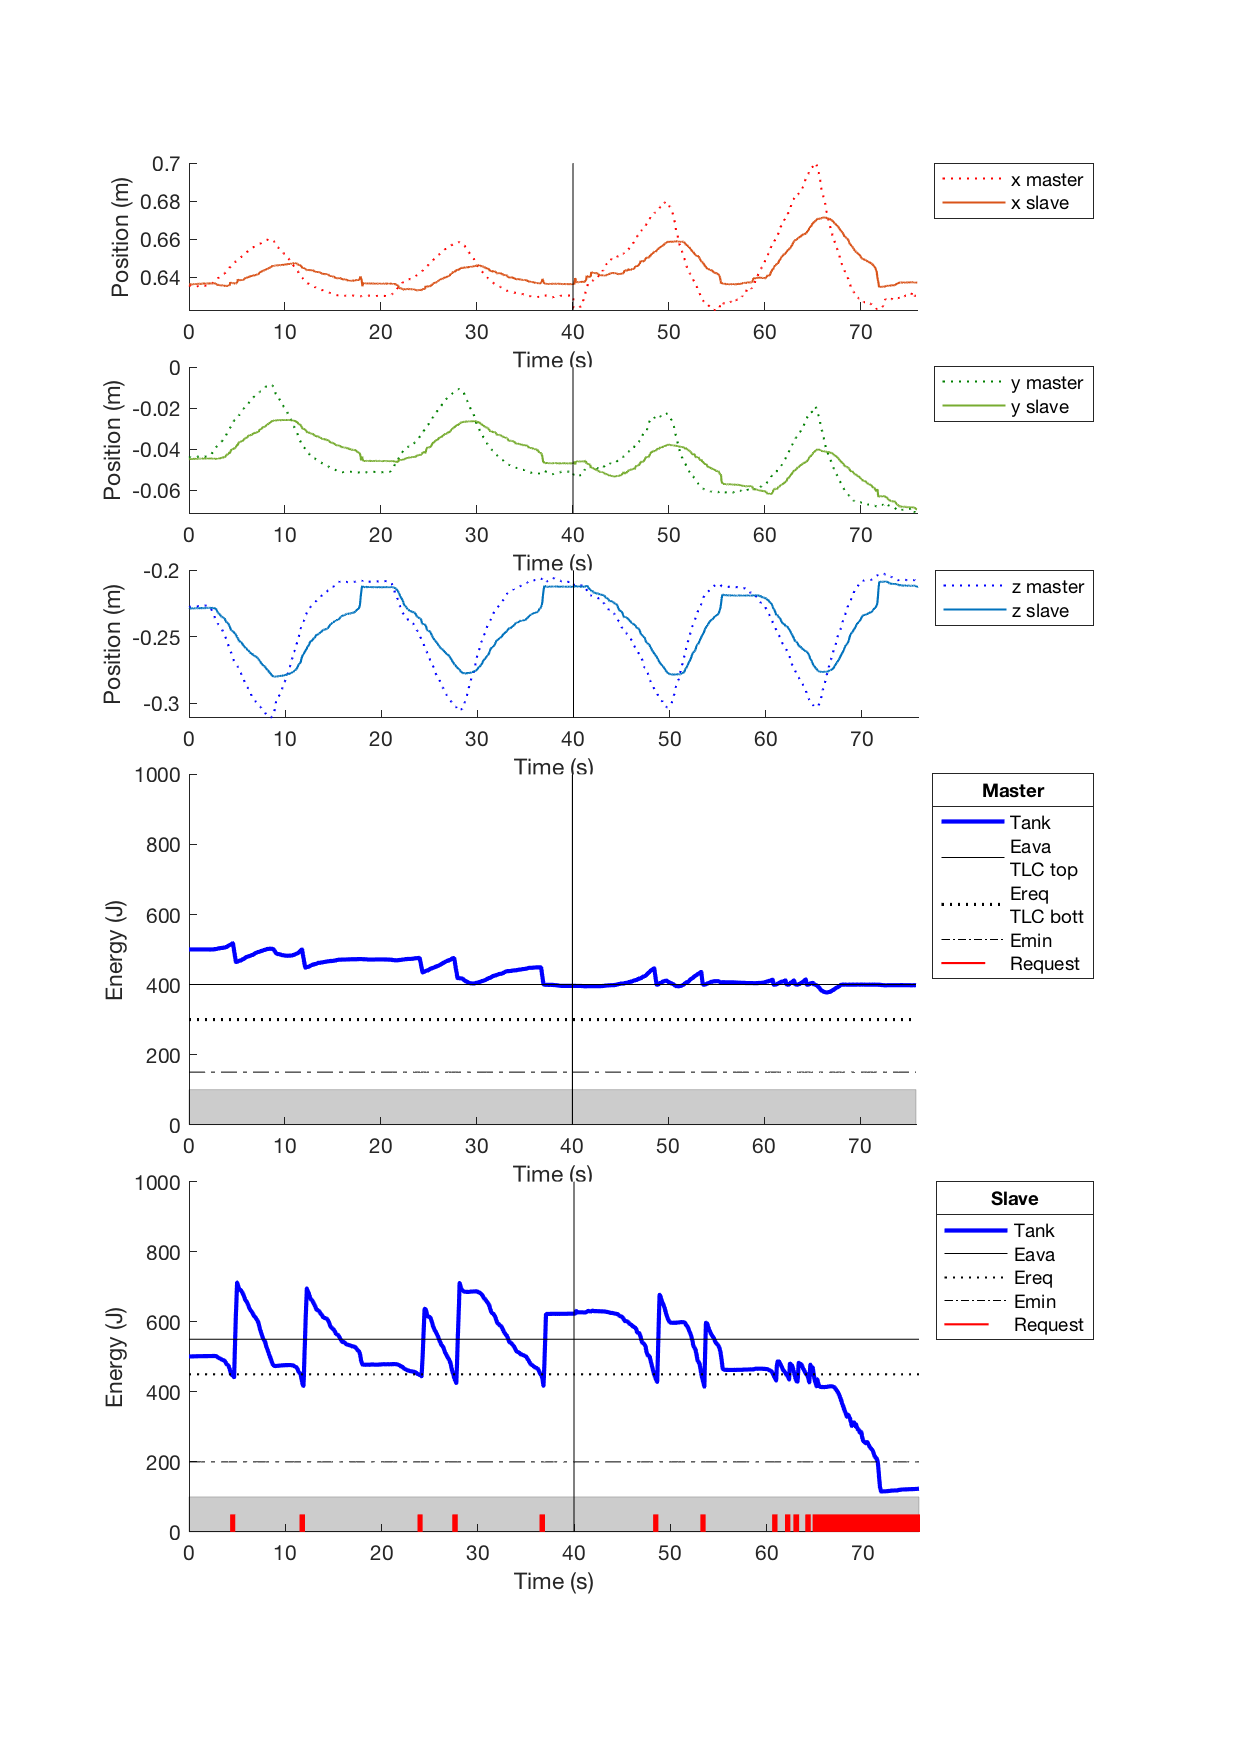
\includegraphics[width=\textwidth, keepaspectratio]{plots/pp45Delay/Position.pdf}
		\caption{Position tracking with 45° insertion approach. P-P control architecture with 0.2s RTT delay.}
		\label{graph:pp45Delay/Position}
	\end{figure}
\end{center}
\begin{center}
	\begin{figure}
		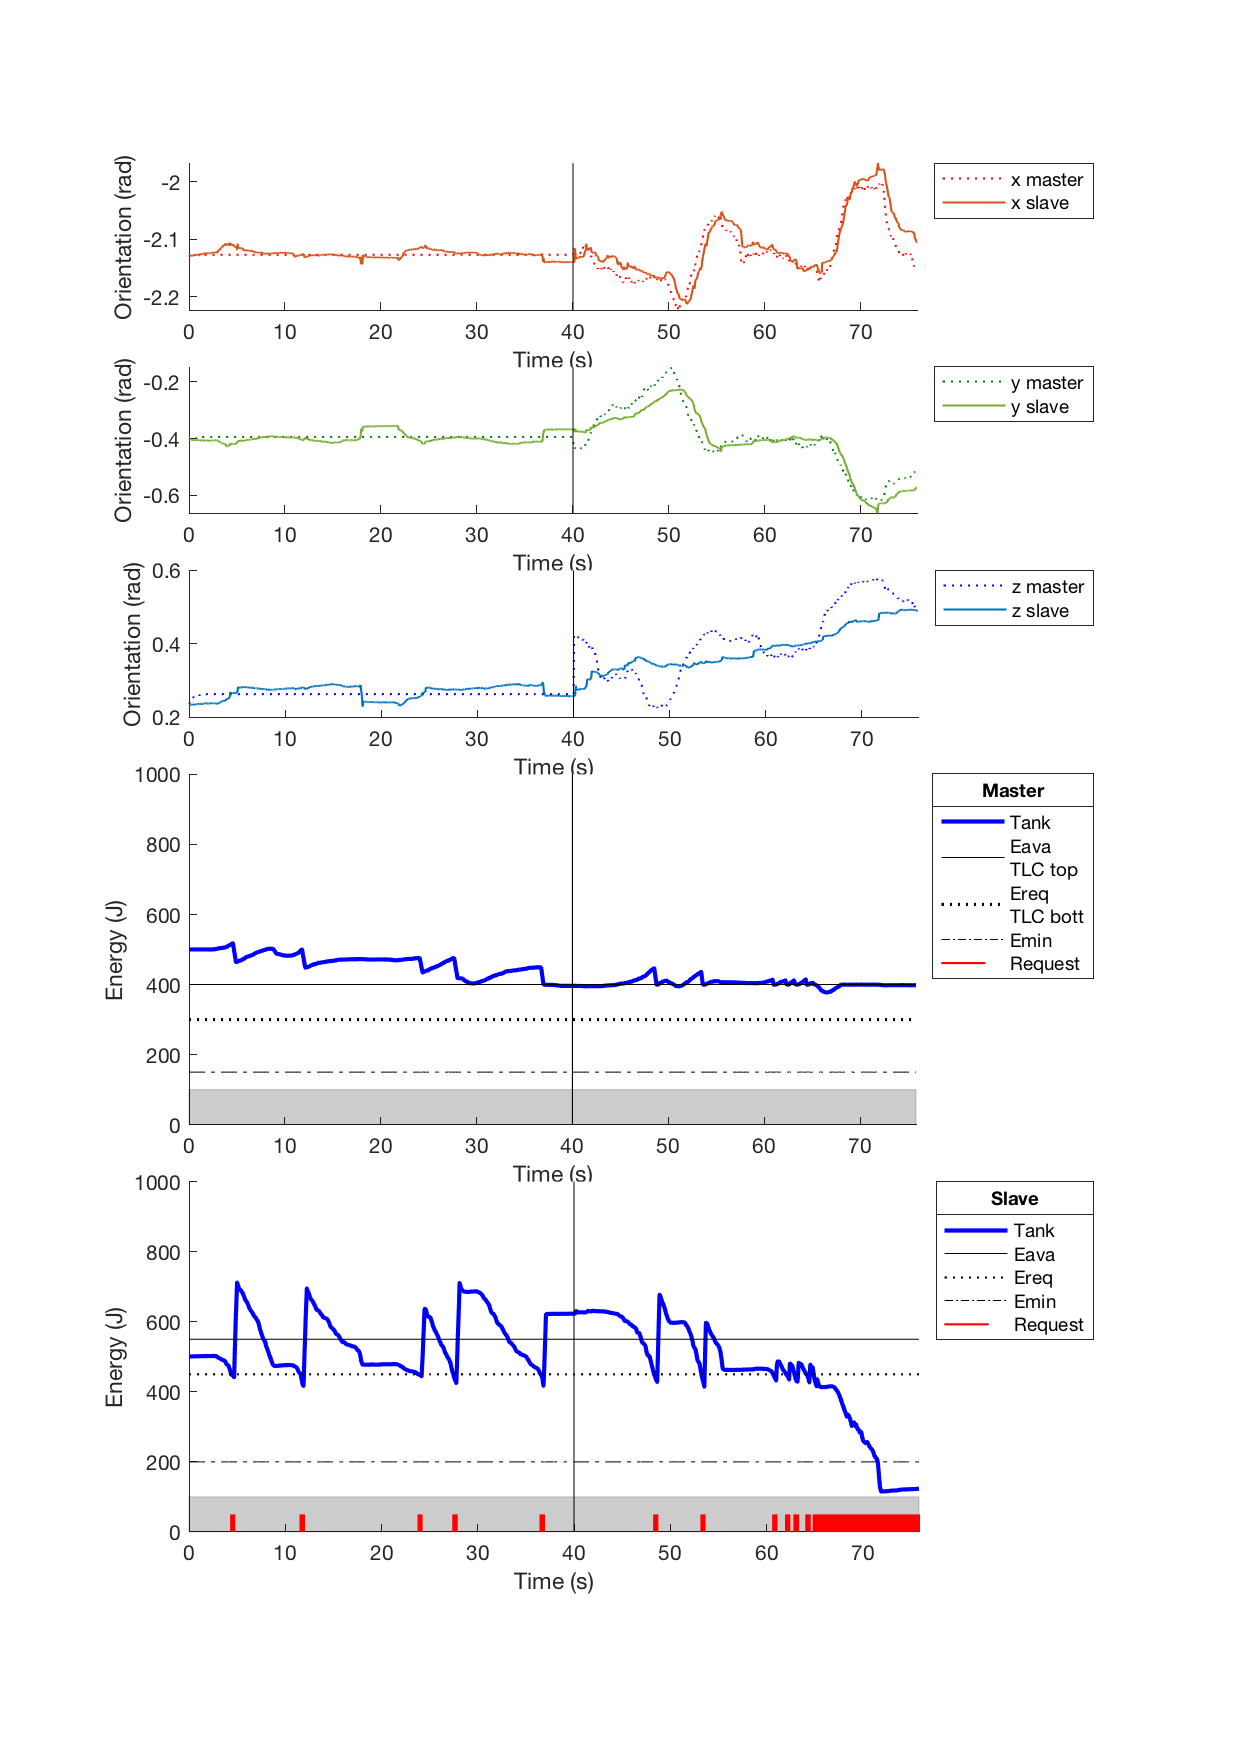
\includegraphics[width=\textwidth, keepaspectratio]{plots/pp45Delay/Orientation.pdf}
		\caption{Orientation tracking with 45° insertion approach. P-P control architecture with 0.2s RTT delay.}
		\label{graph:pp45Delay/Orientation}
	\end{figure}
\end{center}
\begin{center}
	\begin{figure}
		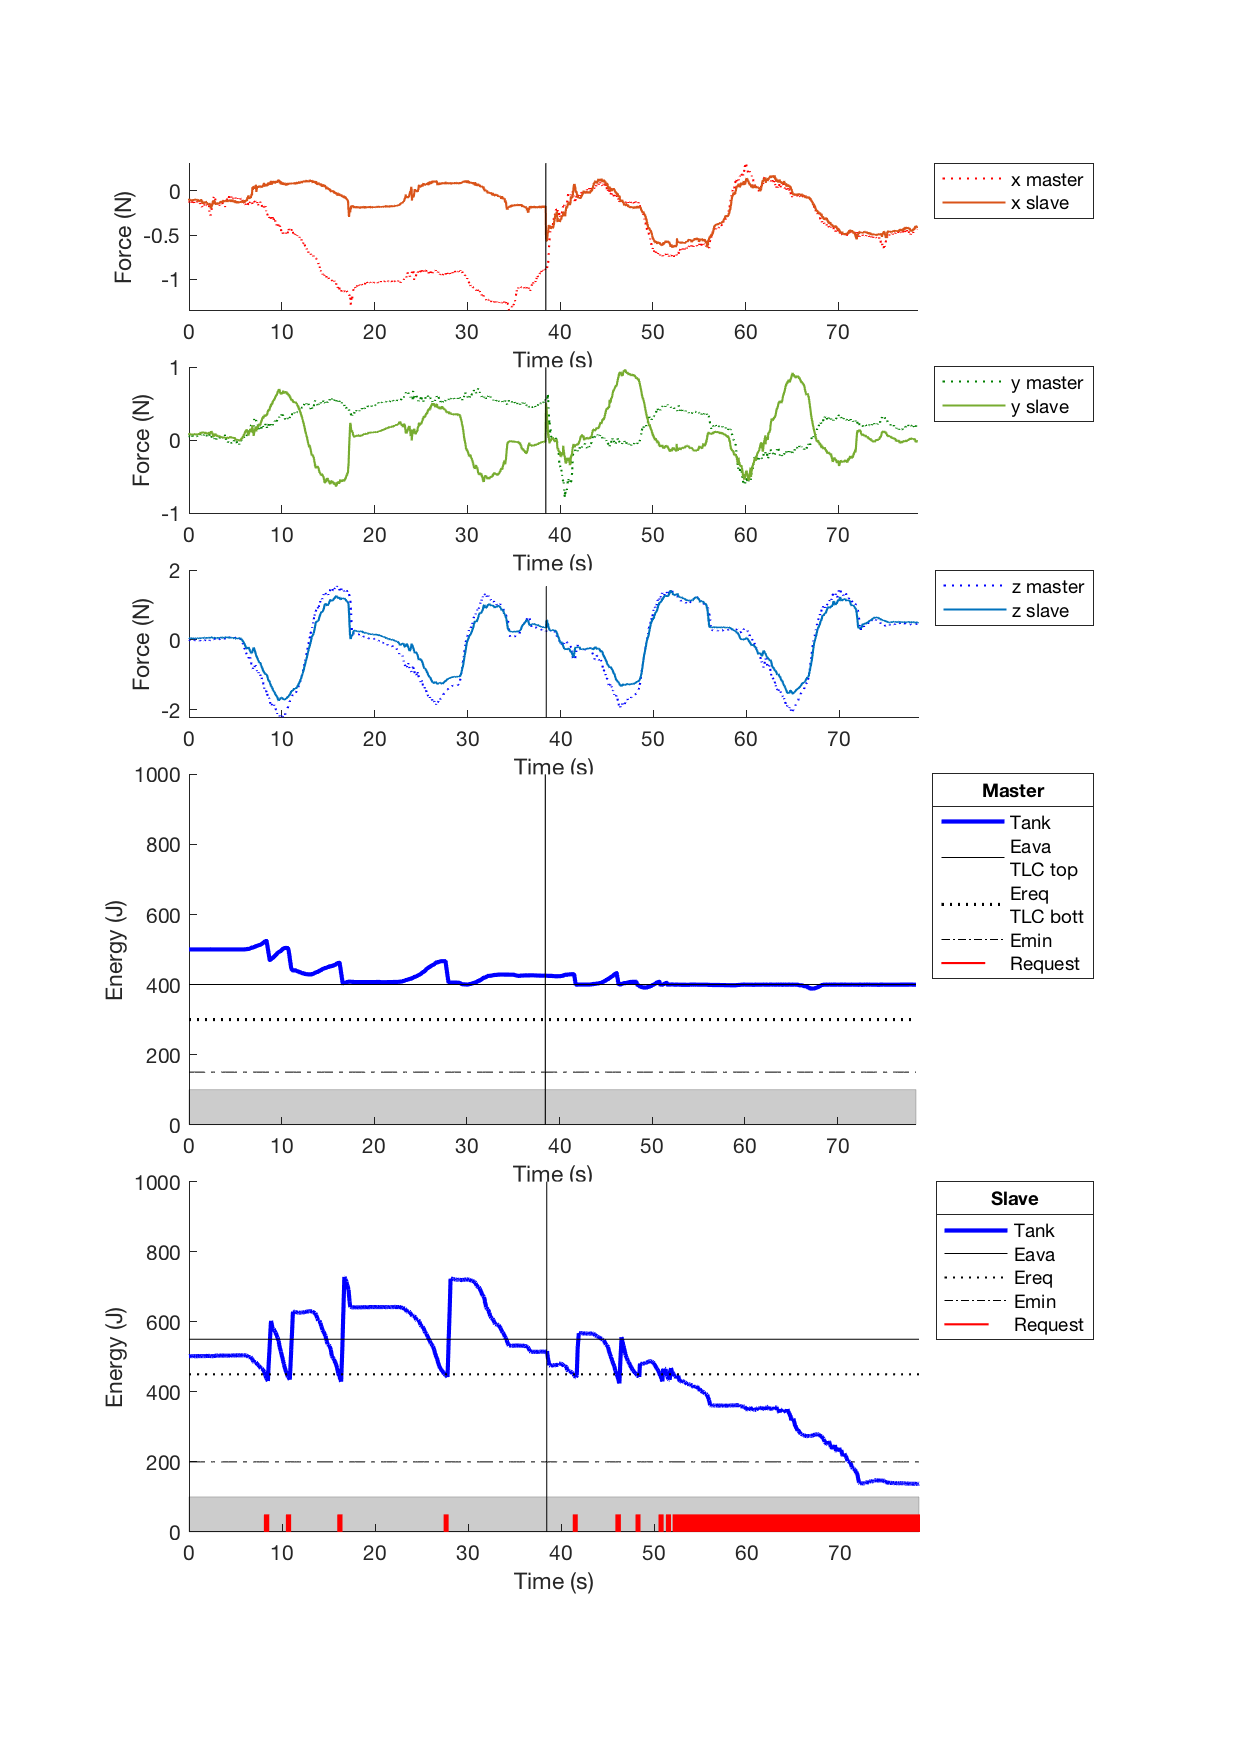
\includegraphics[width=\textwidth, keepaspectratio]{plots/pp90Delay/Force.pdf}
		\caption{Force tracking with 45° insertion approach. P-P control architecture with 0.2s RTT delay.}
		\label{graph:pp45Delay/Force}
	\end{figure}
\end{center}
\newpage
\section{Position-Force}
The last set of experiments are on the Position-Force teleoperation architecture.
The experimental setup has been tuned with the parameters showed in \tablename{ \ref{PFparam}} 
which are described in Sections \ref{sec:HamWithTank} and \ref{Two-Layer-Approach}.
Because of the P-F architecture, the force commanded at master side is scaled by the $K_{f}$ gain.
As done with P-P architecture, we choose to show the slave interaction force in the master reference frame scaled by $K_{f}$.
\begin{table}
	\centering
	\begin{tabular}{llccc}
		\toprule
		&  & Slave & Master & $\mathrm{Master_{pilot}}$ \\ 
		%%\cline{3-5}
		
		\cmidrule{3-5}
		\multirow{2}*{Position PD} &$K_{p_{pos}}$ & 500.0 &  & 50.0\\
		& $K_{d_{pos}}$ & 5.0 & 0.15 & 0.15\\
		\midrule
		\multirow{2}*{Orientation PD} &$K_{p_{ang}}$ & 0.0 &  & 0.0\\
		& $K_{d_{ang}}$ & 0.06 & 0.0 & 0.0 \\ 
		\midrule
		Force Gain& $K_{f}$ &  & 0.5 & 0.5 \\ 
		\midrule[1pt]
		\multirow{9}*{Passivity Layer} &$\bar{T}$ & 1000.0 & 1000.0 \\
		&$T_{ava}$  & 550 & 400\\
		&$T_{req}$ & 450 & 300\\
		&$T_{TLC_{top}}$ & & 400\\
		&$T_{TLC_{bot}}$ & & 300\\
		&$\varepsilon_{top}$ & 200 & 150\\
		&$\varepsilon_{bot}$ & 100 & 100\\
		&$K_{TLC}$ & &0.07\\
		&Scale Factor ($\alpha/\gamma$) & 1/6 & 6.0\\
		\bottomrule
	\end{tabular} 
\caption[P-F parameters]{System's parameters for the Position-Force architecture}
\label{PFparam}
\end{table}
\newpage
\subsection{Without Delay}
\subsubsection{Free motion}
The free motion test (\figurename s{ \ref{graph:pfFree/Position} to \ref{graph:pfFree/Force}})  shows the behaviour of the system when no interaction of the slave robot with the tissue occurs.\\
In \figurename{ \ref{graph:pfFree/Position}} we can see a good position tracking between the two manipulators. The orientation tracking, as shown in \figurename{ \ref{graph:pfFree/Orientation}}, is less precise than expected. This is due to the limits of the slave robot discussed in Section \ref{sec:free-motion}.

The energy balance in the system is assured through the constant damping at master side explained in Section \ref{sec:position---force-p-f}.  
The master is able to provide enough energy to the slave without draining its tank ss shown in \figurename{ \ref{graph:pfFree/Force}}.
\begin{center}
	\begin{figure}
		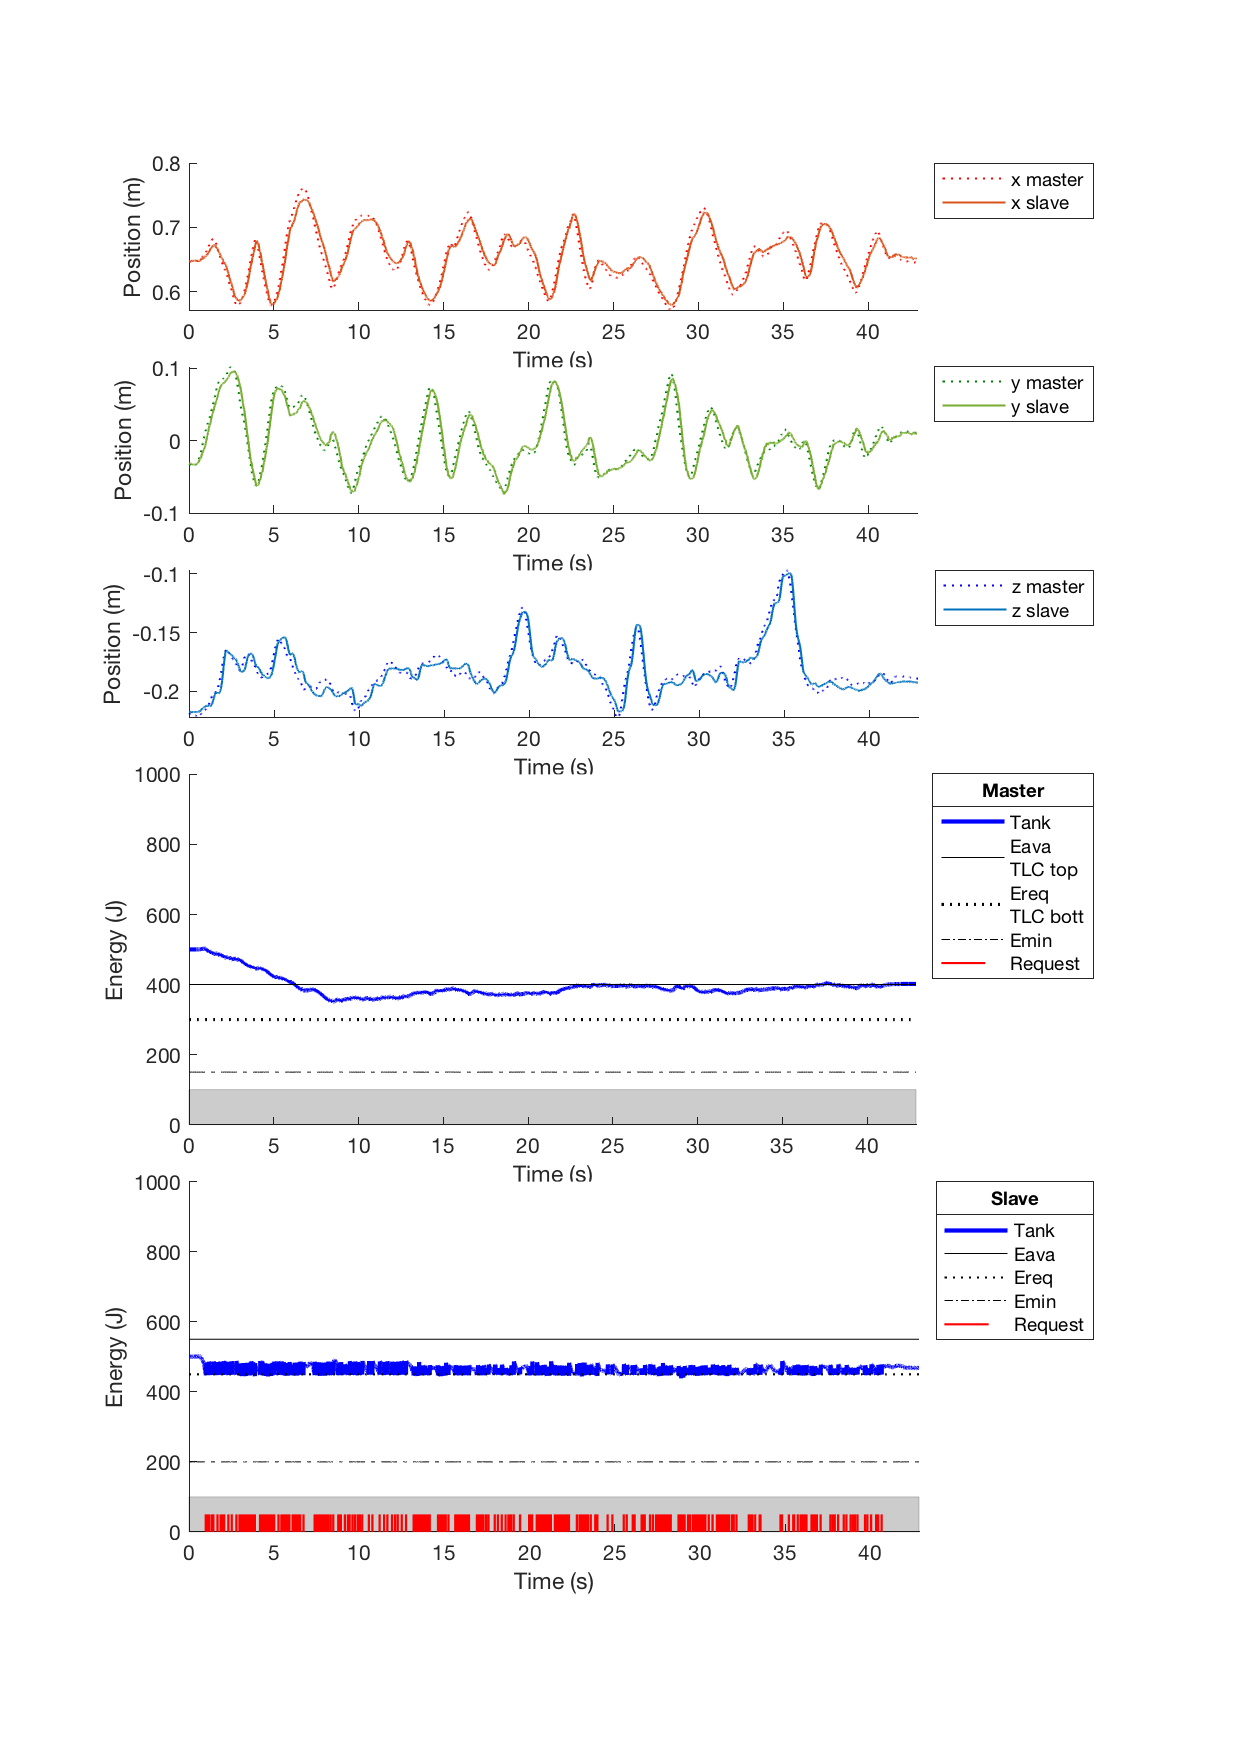
\includegraphics[width=\textwidth, keepaspectratio]{plots/pfFree/Position.pdf}
		\caption{Position tracking in free motion. P-F control architecture without delay.}
		\label{graph:pfFree/Position}
	\end{figure}
\end{center}
\begin{center}
	\begin{figure}
		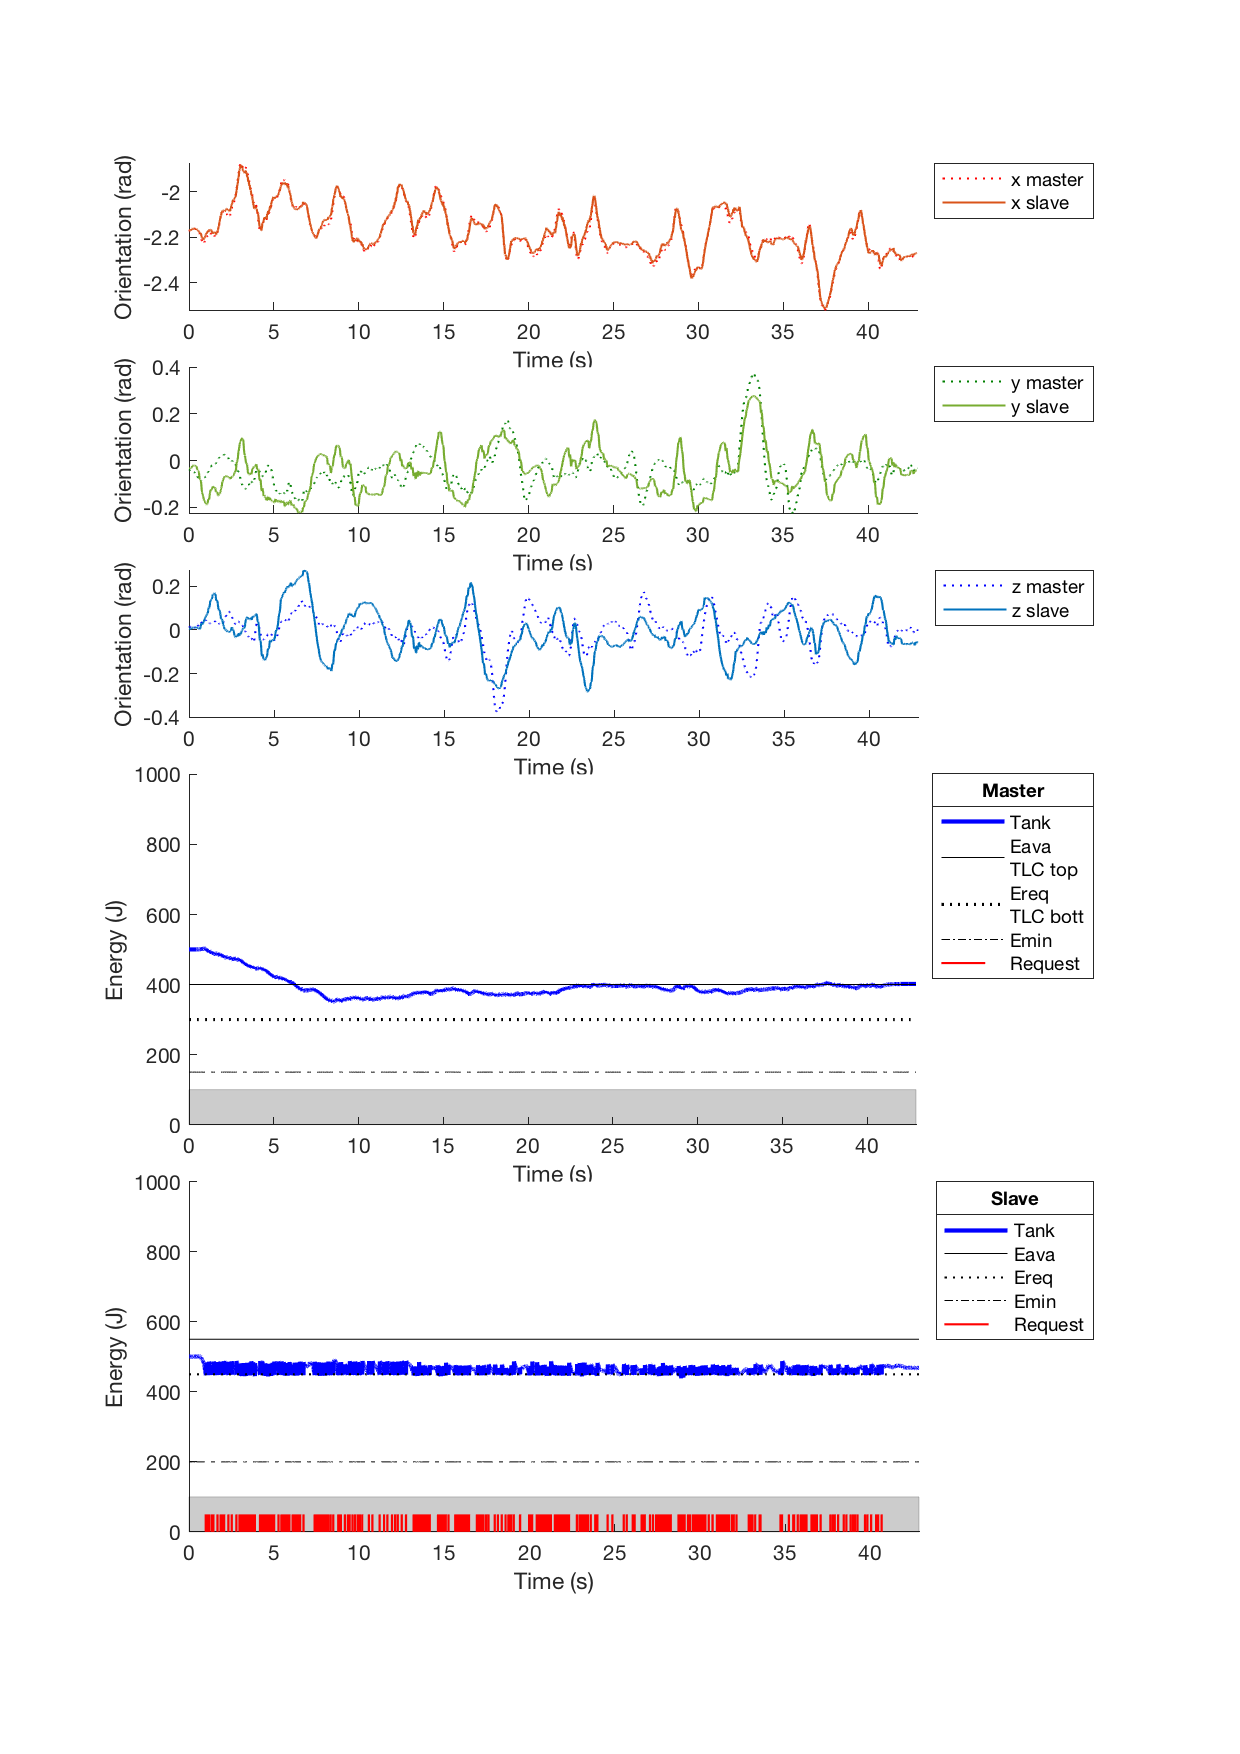
\includegraphics[width=\textwidth, keepaspectratio]{plots/pfFree/Orientation.pdf}
		\caption{Orientation tracking in free motion. P-F control architecture without delay.}
		\label{graph:pfFree/Orientation}
	\end{figure}
\end{center}
\begin{center}
	\begin{figure}
		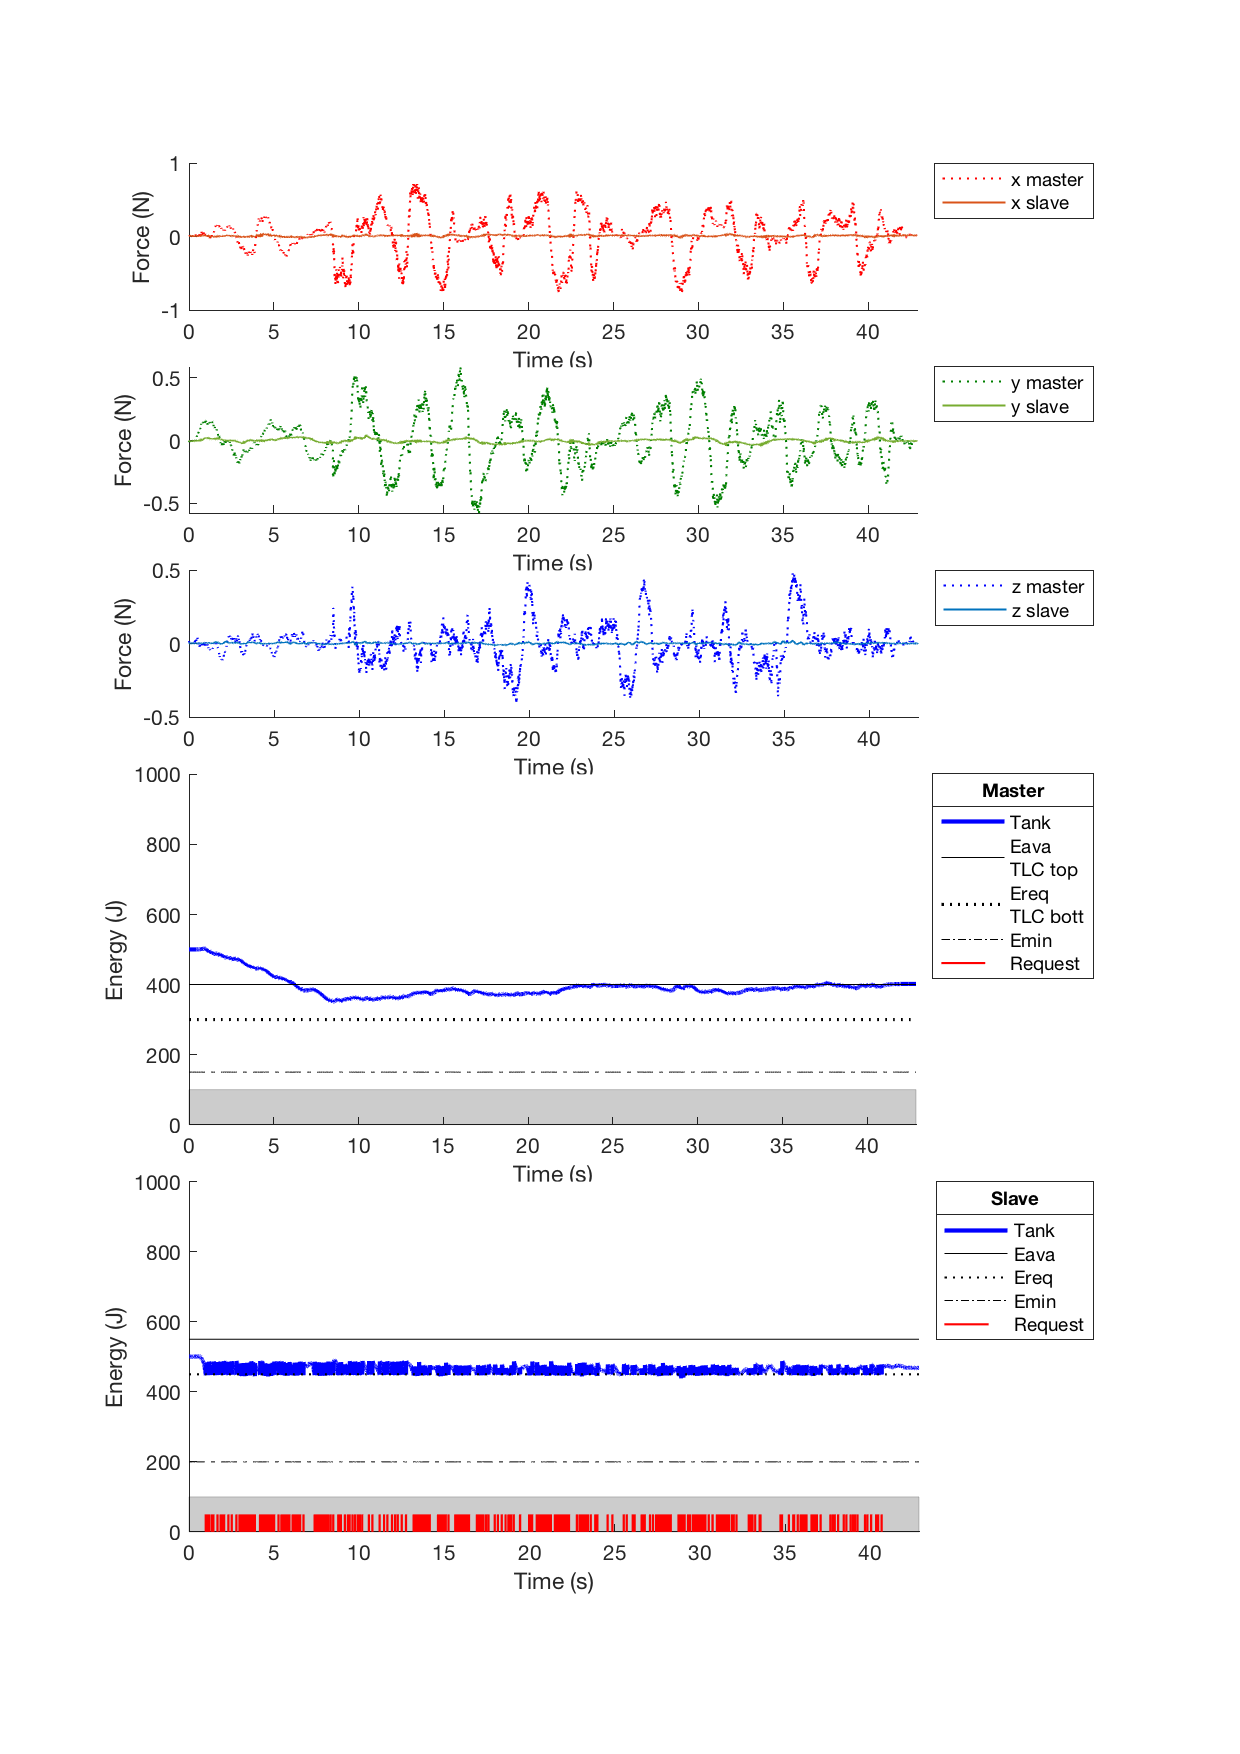
\includegraphics[width=\textwidth, keepaspectratio]{plots/pfFree/Force.pdf}
		\caption{Orientation tracking in free motion. P-F control architecture without delay.}
		\label{graph:pfFree/Force}
	\end{figure}
\end{center}
\newpage
\subsubsection{Insertion with 90° approaching angle}
In this test  (\figurename s{ \ref{graph:pf90/Position} to \ref{graph:pf90/Force}}) the first puncture have been executed with the standard controller and the other two within the \textit{Pilot Mode}.
The change of controller at time 20.0s is highlighted by a vertical line.

In the first puncture we can se some unwanted movements due to the reaction force exerted on the needle shaft by the phantom tissue when the needle advance varying its orientation.
We previously discussed this behaviour in Section \ref{sec:insertion-with-90-approaching-angle1}.\\
The component of that force that implies a translation is felt by the operator who try to correct the behaviour. However the lack of actuation on the orientation gives only a partial feedback.\\
Due to to the tissue constraints the operators reaction easily produces an excessive movement that has to be balanced again. This undesired behaviour could be compensated with the \textit{Pilot controller} that preserves the force feedback along $z$. The \textit{Pilot controller} for the P-F teleoperation architecture is explained in Section \ref{sec:position---force-p-f}.\\
The forces on $x-y$ at the slave can be explained due to the errors in position and orientation. On the master these forces are due to the violation of the virtual trajectory constraints by the operator.
What we can notice is the very good tracking of the force feedback provided in $z$ due to nature of the architecture.
\begin{center}
	\begin{figure}
		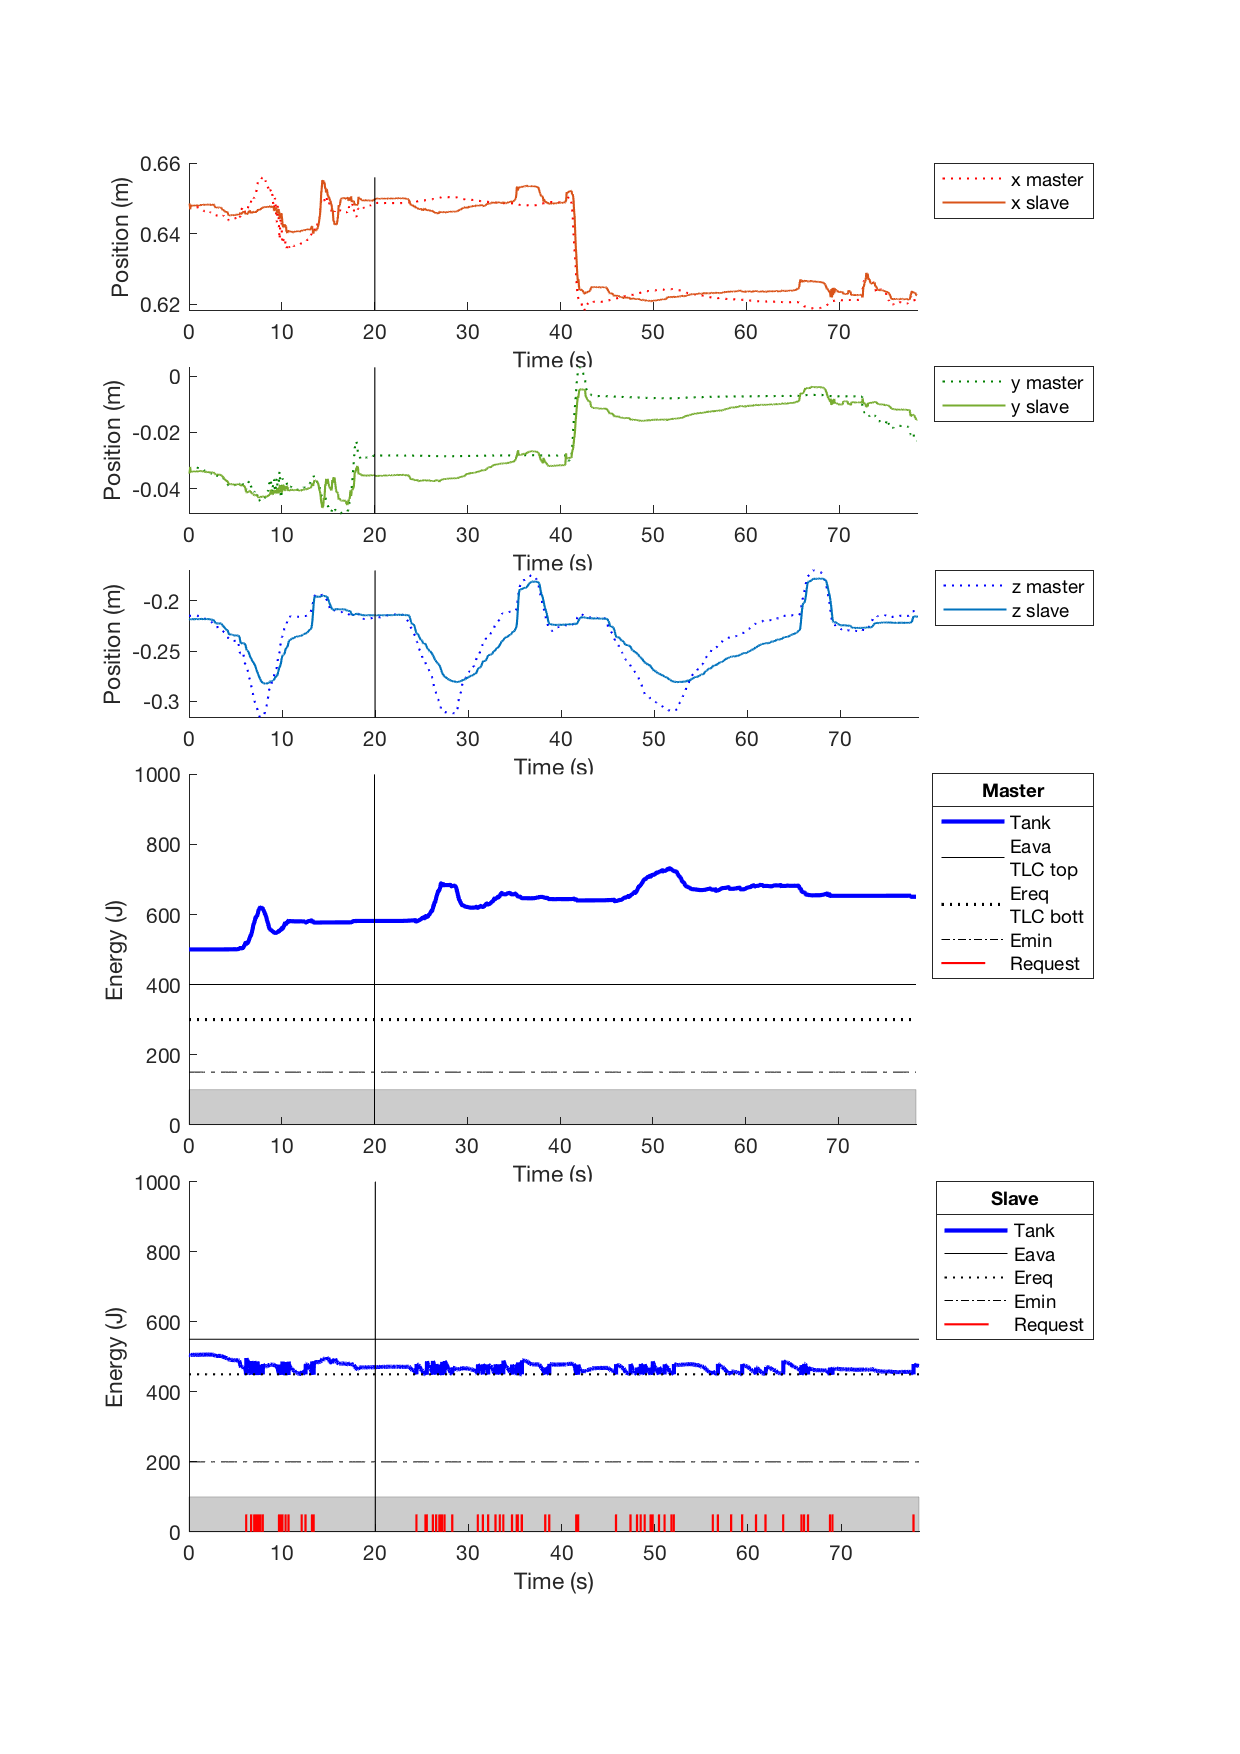
\includegraphics[width=\textwidth, keepaspectratio]{plots/pf90/Position.pdf}
		\caption{Position tracking with 90° insertion approach. P-F control architecture without delay.}
		\label{graph:pf90/Position}
	\end{figure}
\end{center}
\begin{center}
	\begin{figure}
		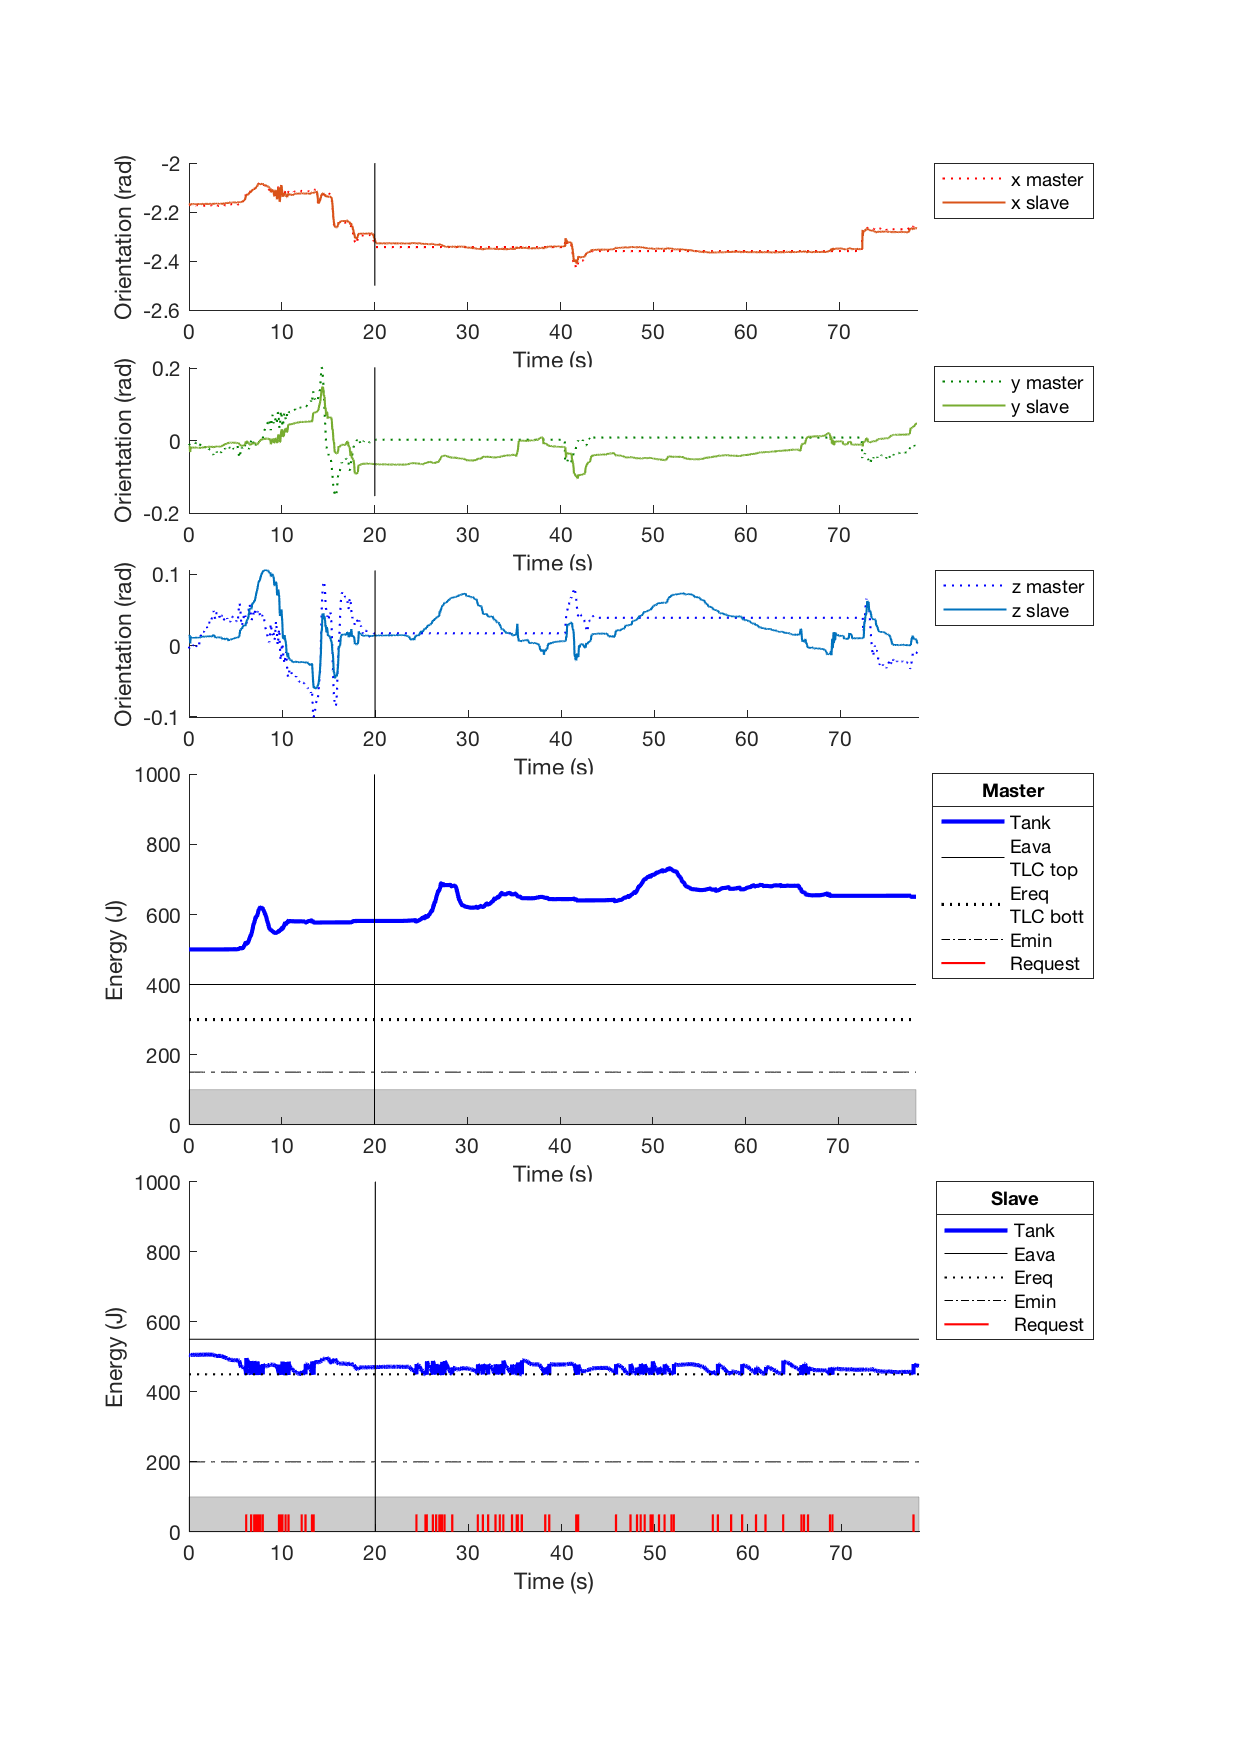
\includegraphics[width=\textwidth, keepaspectratio]{plots/pf90/Orientation.pdf}
		\caption{Orientation tracking with 90° insertion approach. P-F control architecture without delay.}
		\label{graph:pf90/Orientation}
	\end{figure}
\end{center}
\begin{center}
	\begin{figure}
		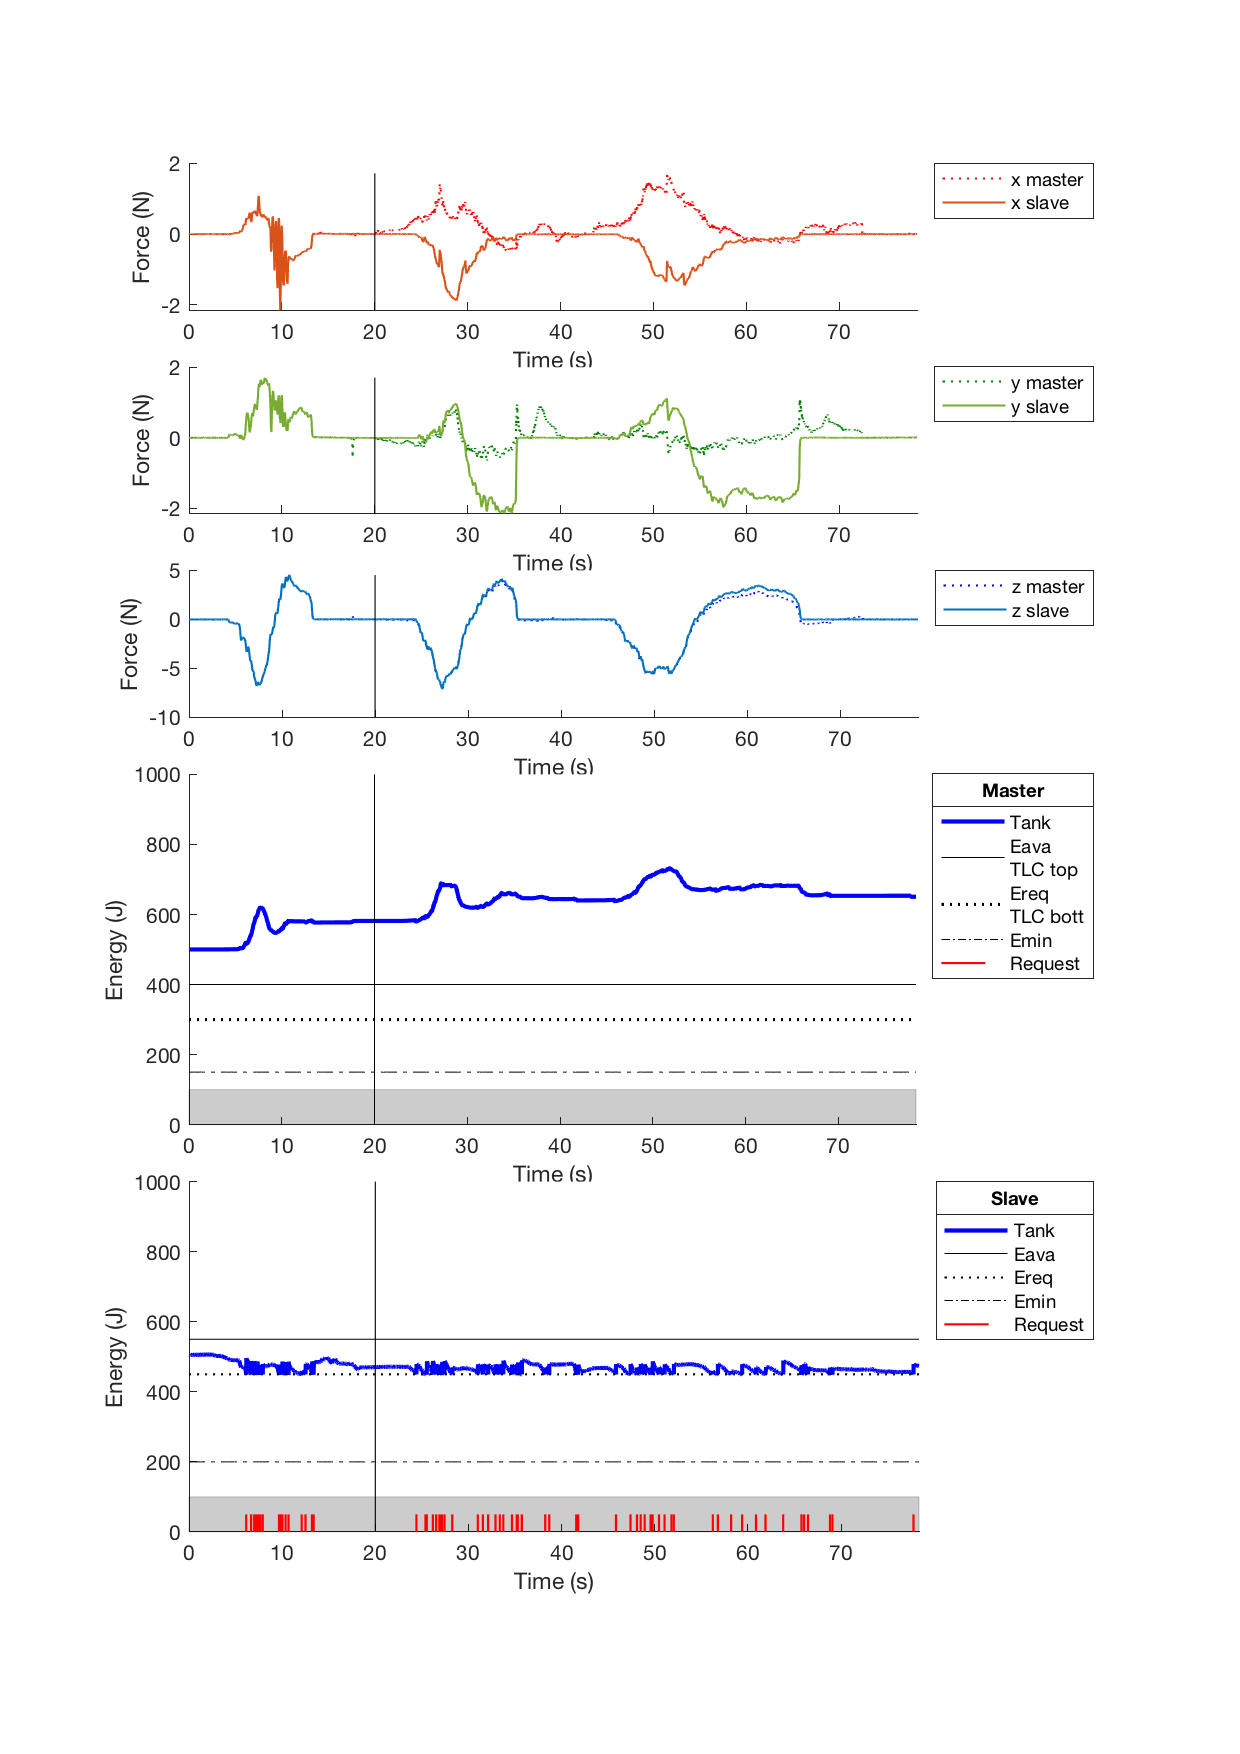
\includegraphics[width=\textwidth, keepaspectratio]{plots/pf90/Force.pdf}
		\caption{Force tracking with 90° insertion approach. P-F control architecture without delay.}
		\label{graph:pf90/Force}
	\end{figure}
\end{center}
\newpage
\subsubsection{Insertion with 45° approaching angle}
In this test  (\figurename s{ \ref{graph:pf90/Position} to \ref{graph:pf90/Force}}) the first puncture has been done within the \textit{Pilot Mode}, the other with the standard controller.
The change of controller at time 23.3s is highlighted by a vertical line.
In this test both the punctures has been executed accurately.
\begin{center}
	\begin{figure}
		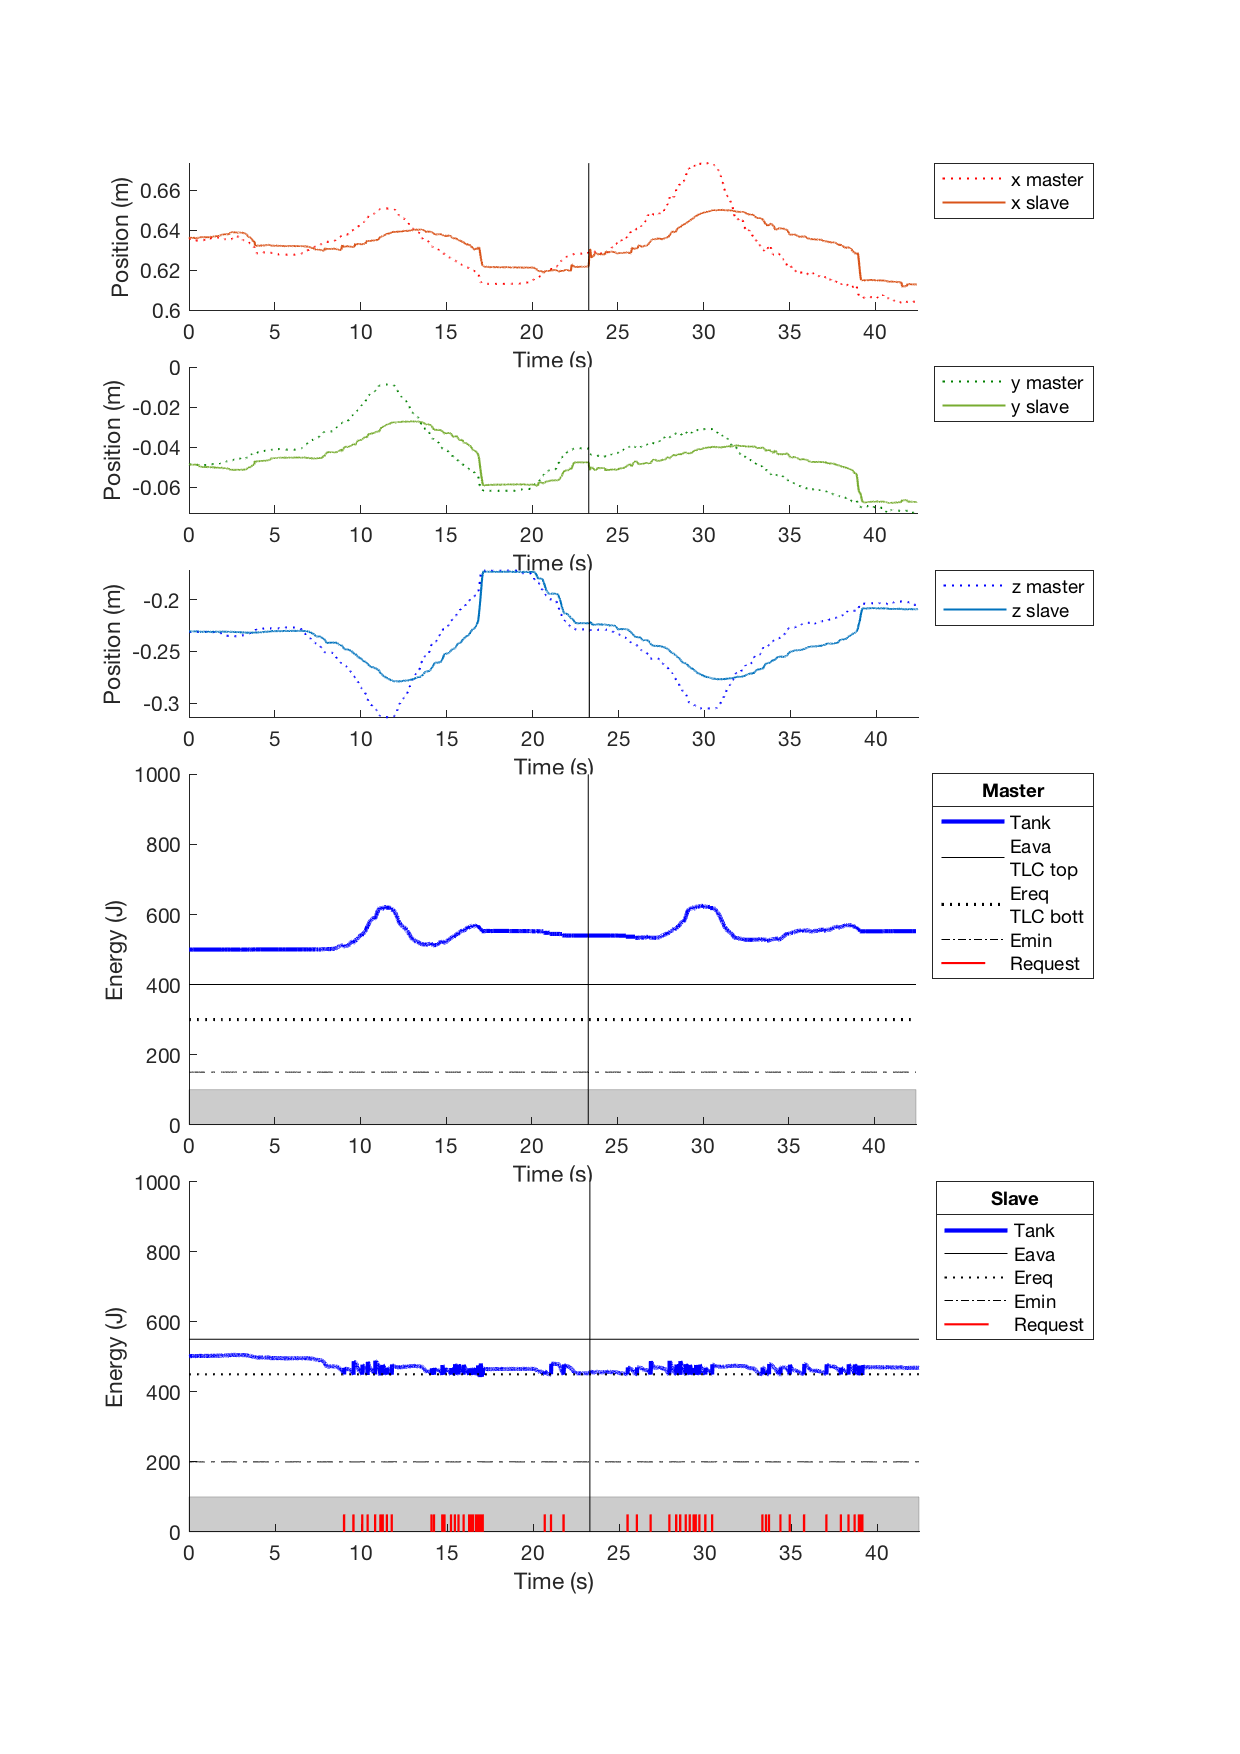
\includegraphics[width=\textwidth, keepaspectratio]{plots/pf45/Position.pdf}
		\caption{Position tracking with 45° insertion approach. P-F control architecture without delay.}
		\label{graph:pf45/Position}
	\end{figure}
\end{center}
\begin{center}
	\begin{figure}
		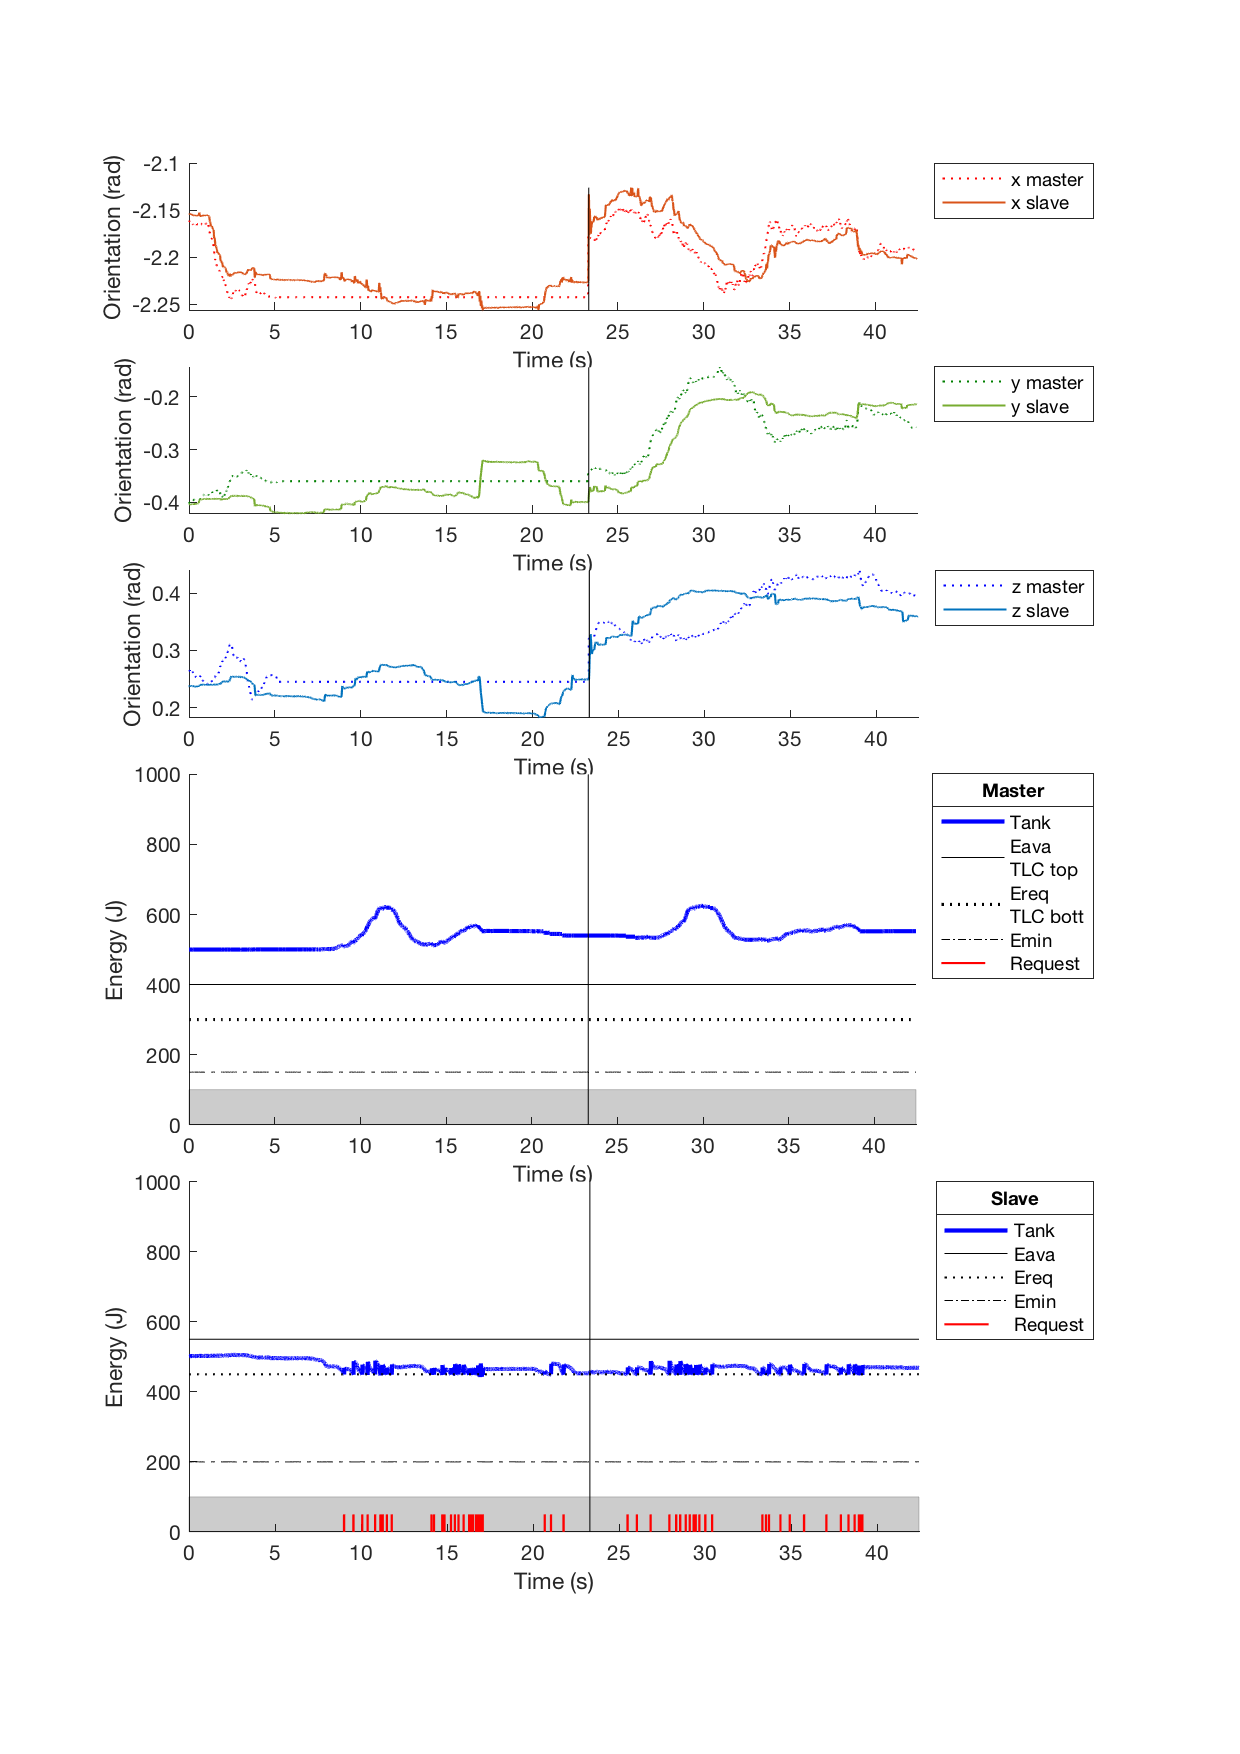
\includegraphics[width=\textwidth, keepaspectratio]{plots/pf45/Orientation.pdf}
		\caption{Orientation tracking with 45° insertion approach. P-F control architecture without delay.}
		\label{graph:pf45/Orientation}
	\end{figure}
\end{center}
\begin{center}
	\begin{figure}
		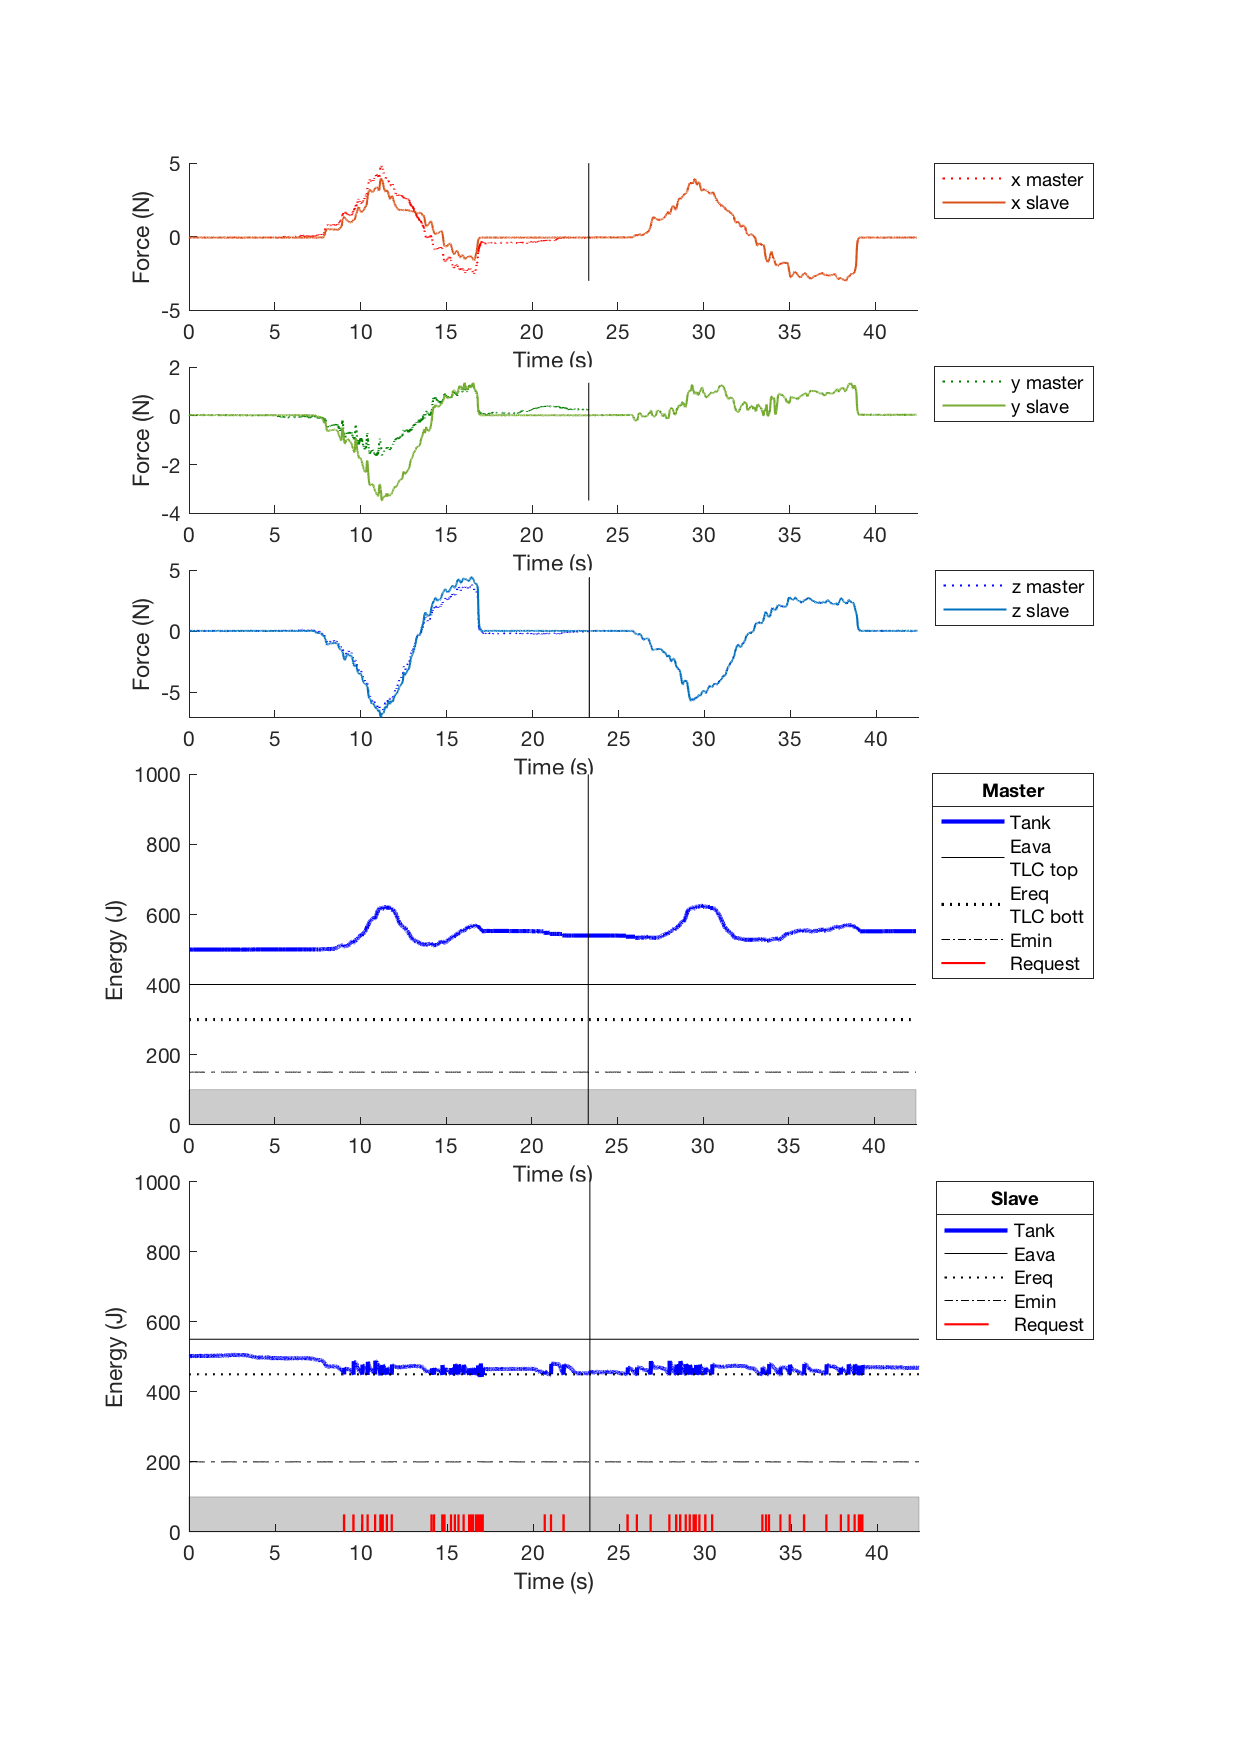
\includegraphics[width=\textwidth, keepaspectratio]{plots/pf45/Force.pdf}
		\caption{Force tracking with 45° insertion approach. P-F control architecture without delay.}
		\label{graph:pf45/Force}
	\end{figure}
\end{center}
\newpage
\subsection{Constant Delay}
\subsubsection{Free motion}
The free motion test has been repeated introducing a constant delay into the communication channel
(\figurename{ \ref{graph:pfFreeDelay/Position} to \ref{graph:pfFreeDelay/Force}}).
The system's  energy behave as described in the delayed P-P architecture.
\begin{center}
	\begin{figure}
		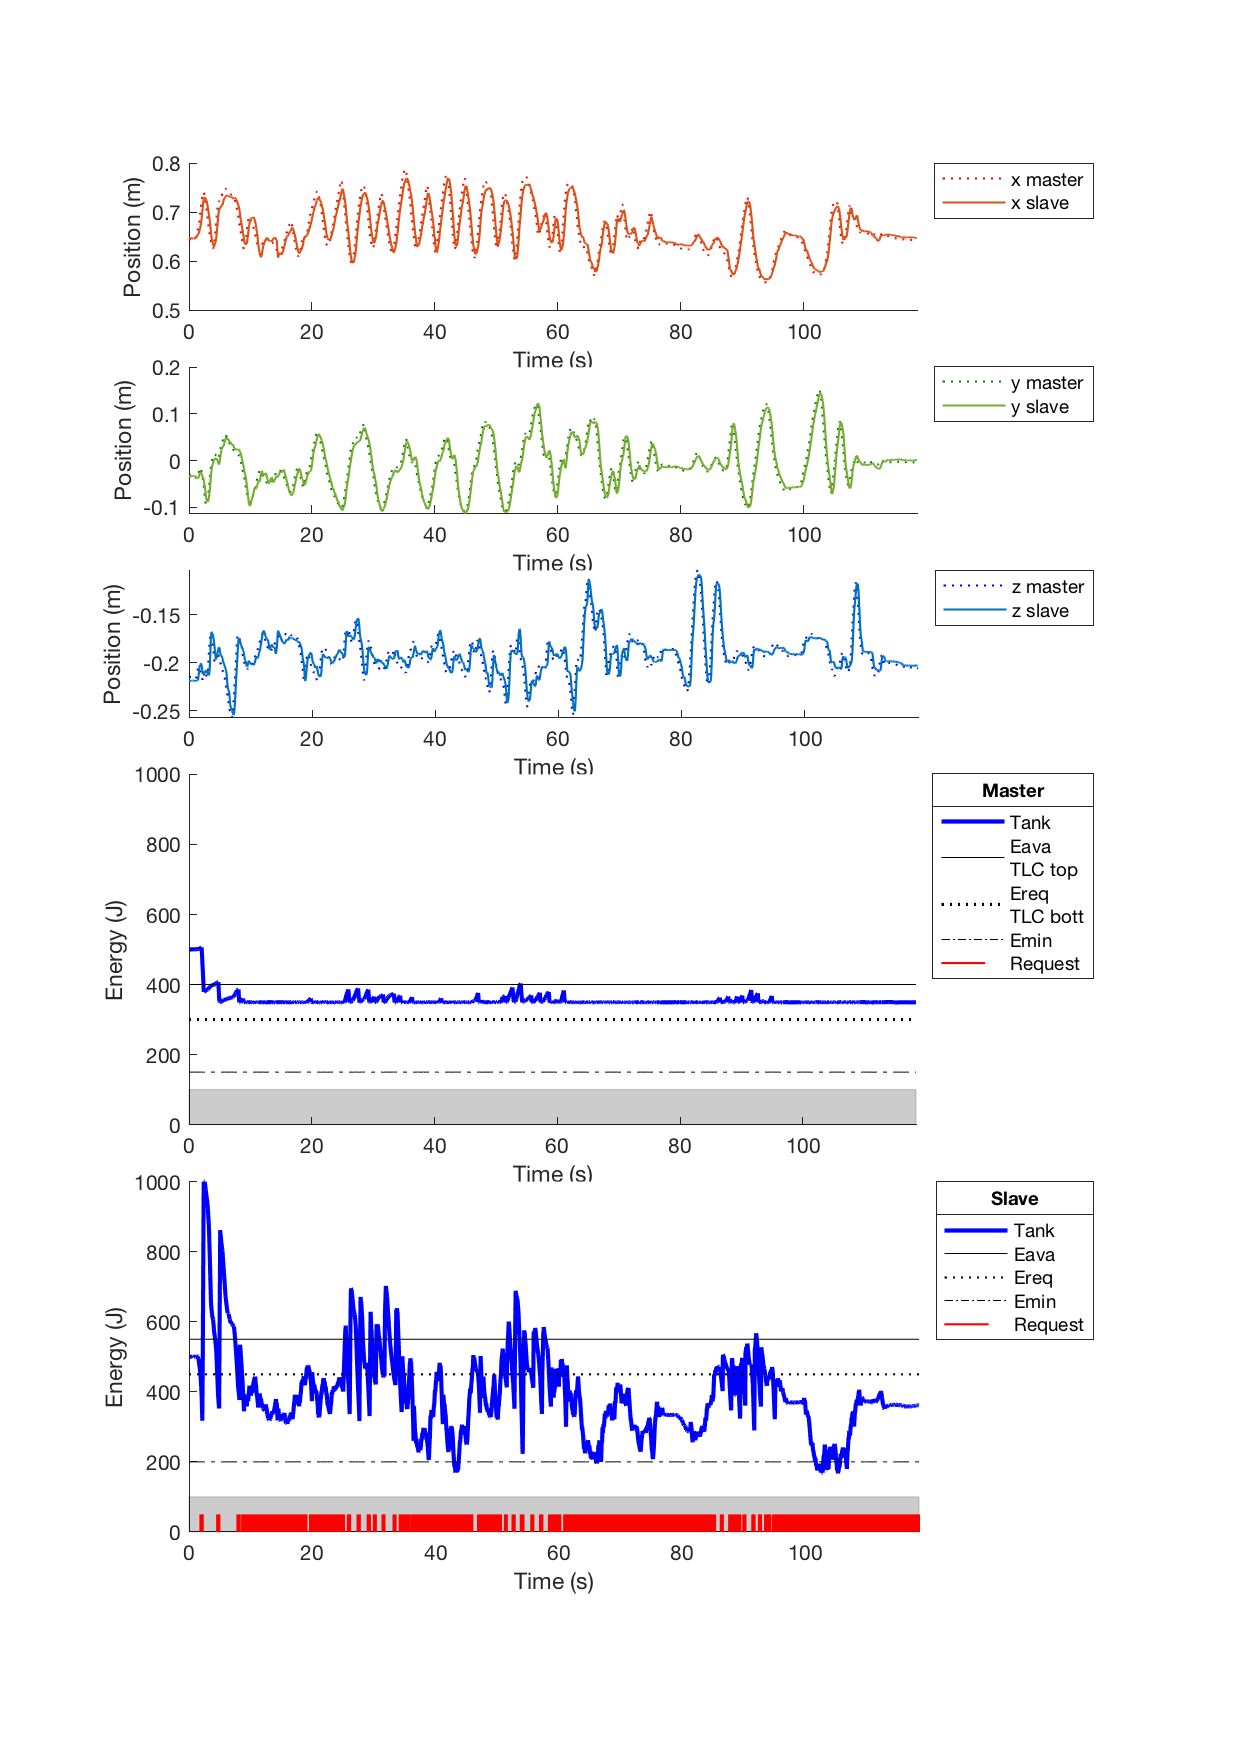
\includegraphics[width=\textwidth, keepaspectratio]{plots/pfFreeDelay/Position.pdf}
		\caption{Position tracking in free motion. P-F control architecture with 0.2s RTT delay.}
		\label{graph:pfFreeDelay/Position}
	\end{figure}
\end{center}
\begin{center}
	\begin{figure}
		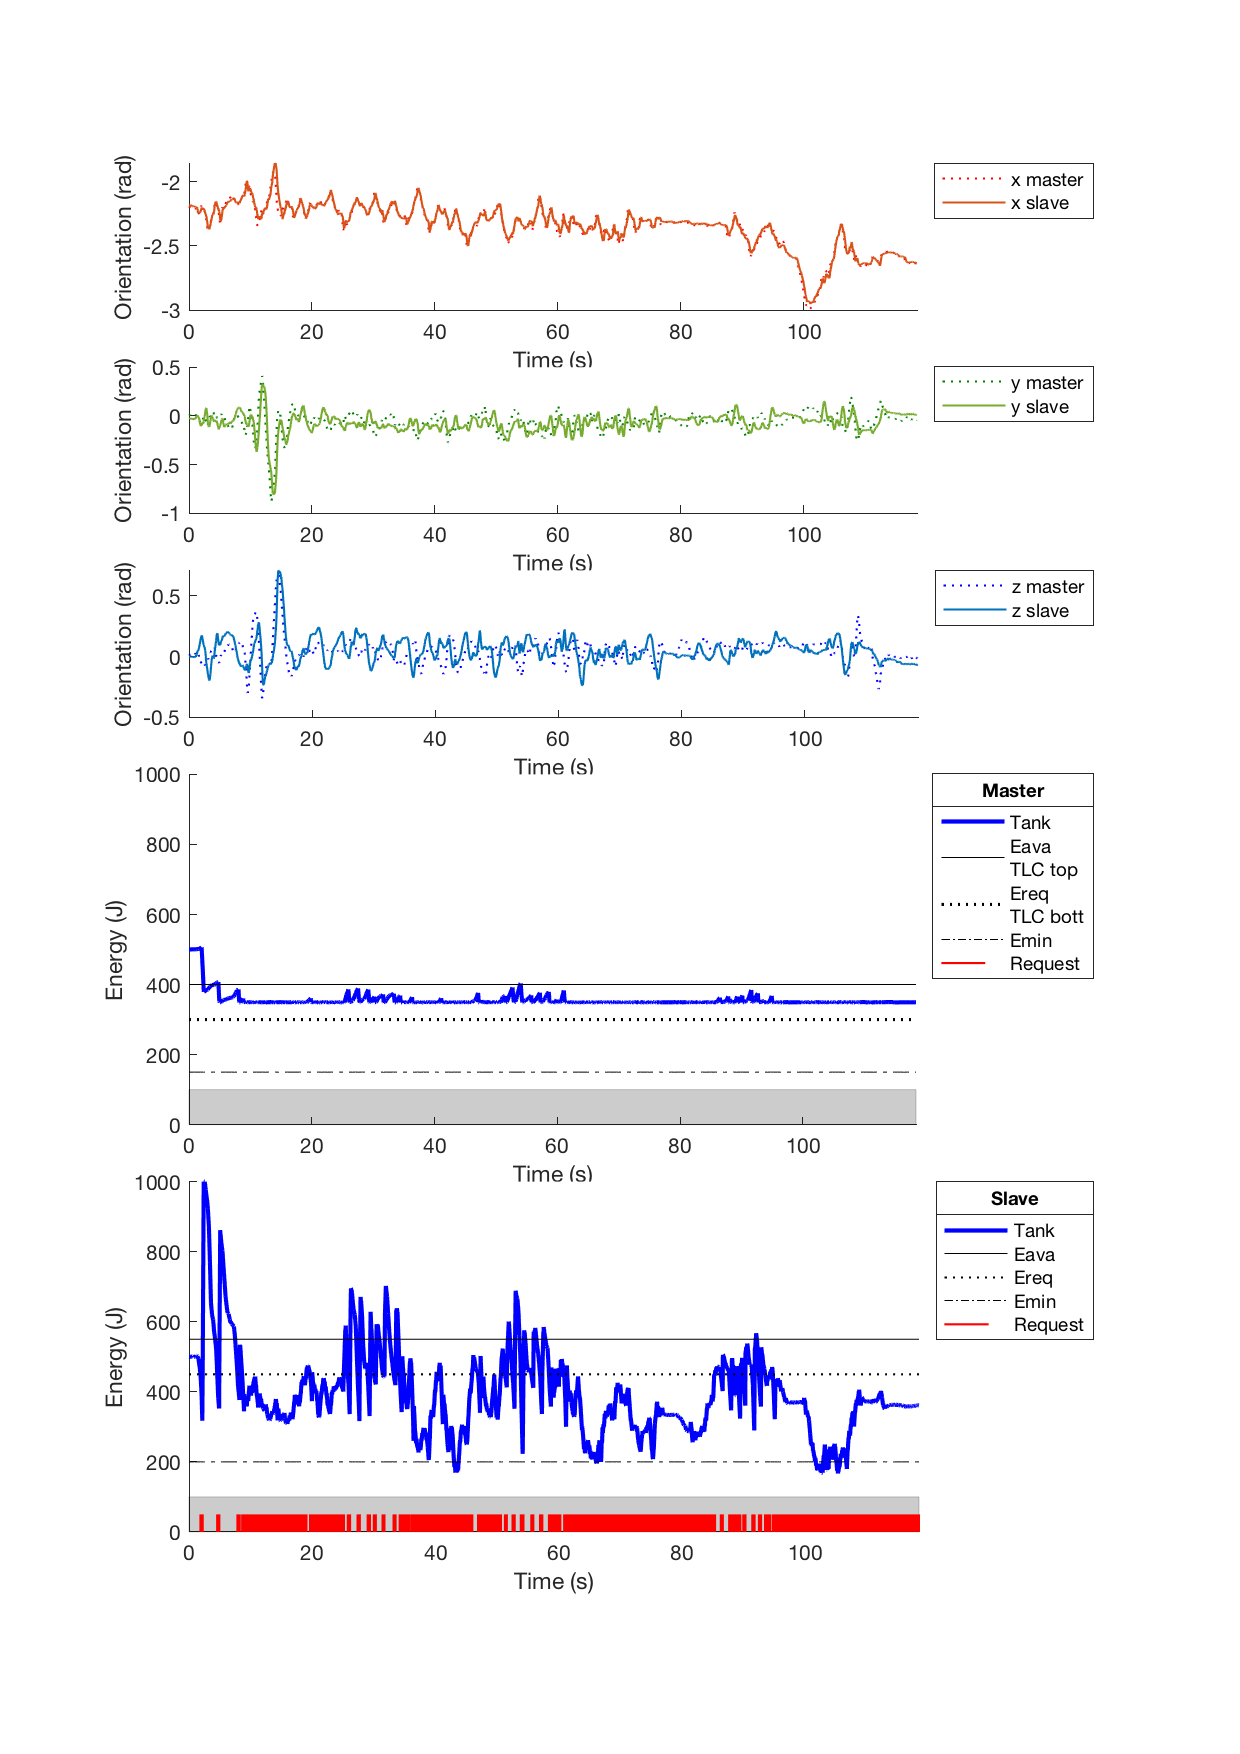
\includegraphics[width=\textwidth, keepaspectratio]{plots/pfFreeDelay/Orientation.pdf}
		\caption{Orientation tracking in free motion. P-F control architecture with 0.2s RTT delay.}
		\label{graph:pfFreeDelay/Orientation}
	\end{figure}
\end{center}
\begin{center}
	\begin{figure}
		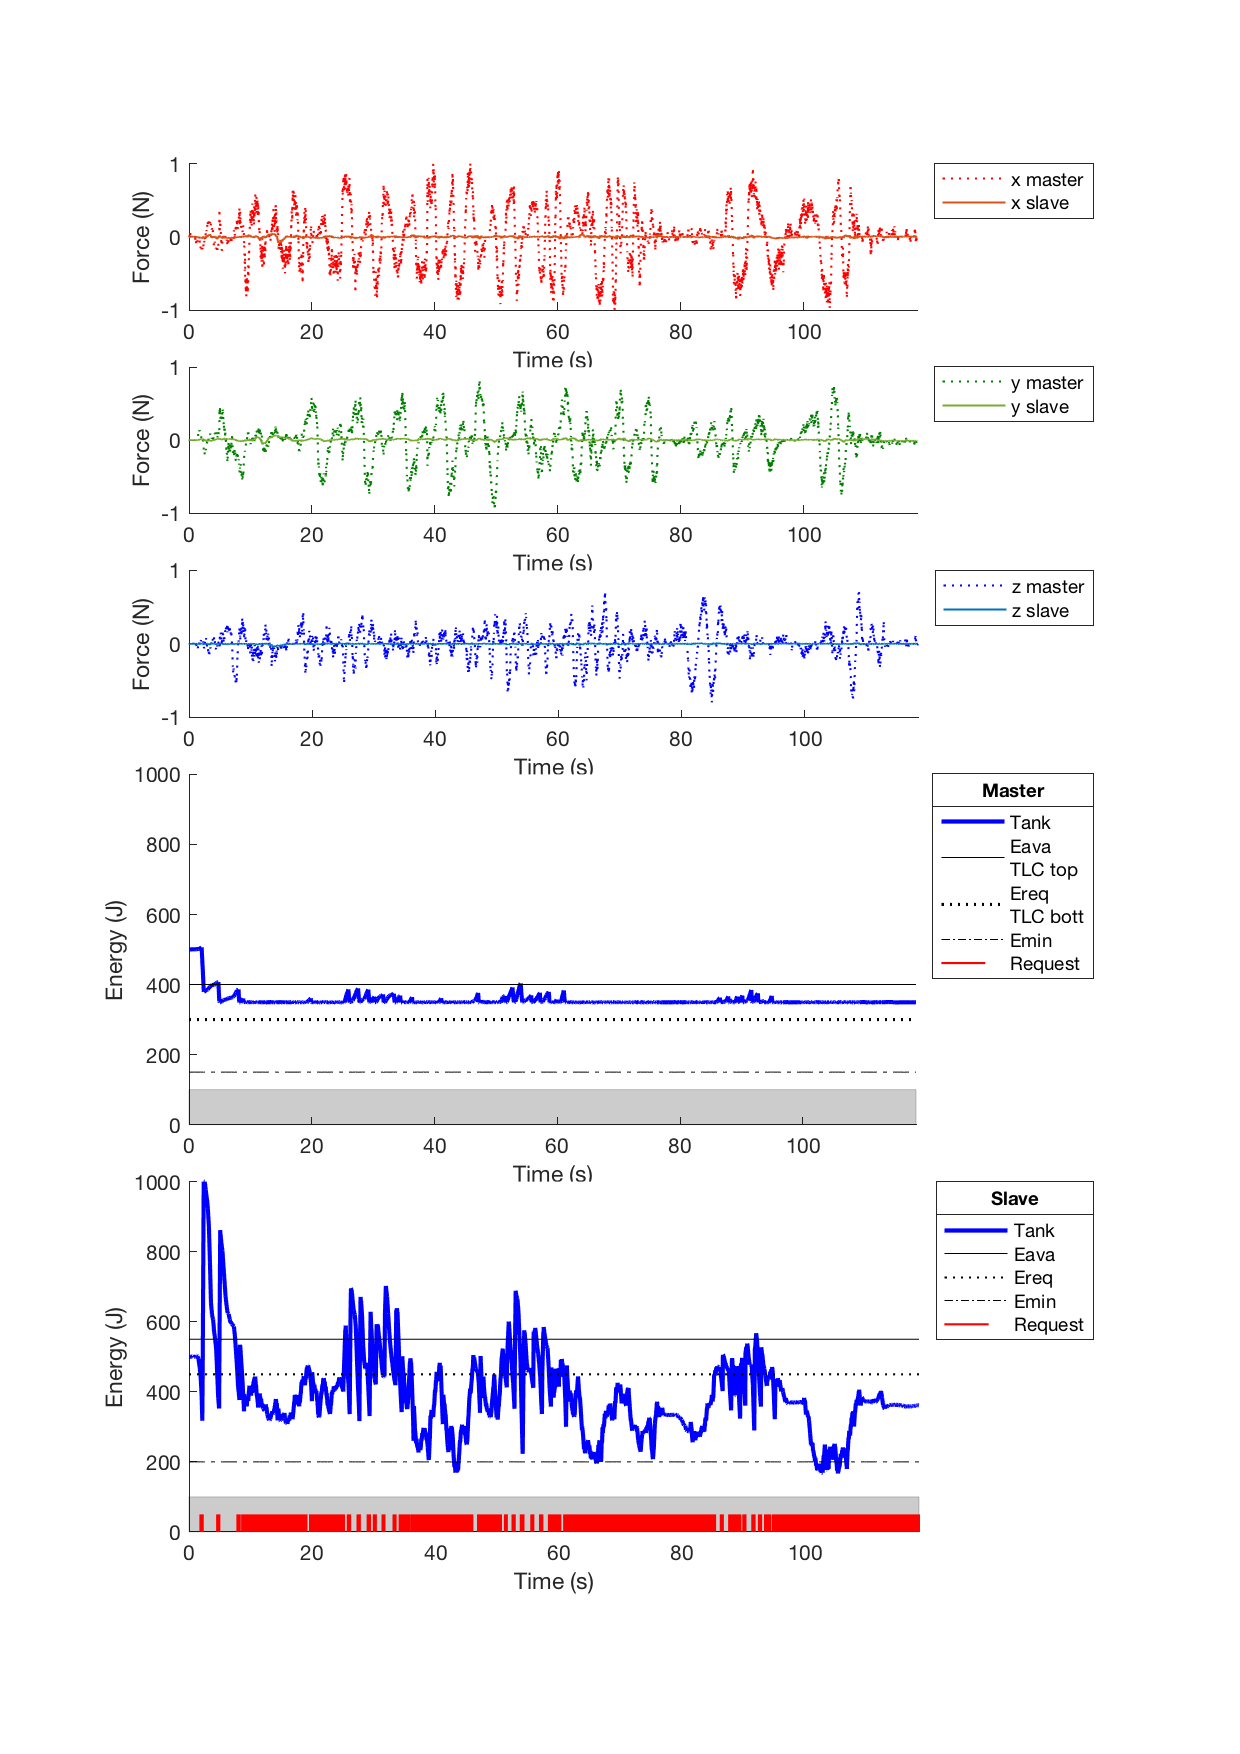
\includegraphics[width=\textwidth, keepaspectratio]{plots/pfFreeDelay/Force.pdf}
		\caption{Force tracking in free motion. P-F control architecture with 0.2s RTT delay.}
		\label{graph:pfFreeDelay/Force}
	\end{figure}
\end{center}
\newpage
\subsubsection{Insertion with 90° approaching angle}\label{sec:insertion-with-90-approaching-angle}
In this test  (\figurename{ \ref{graph:pf90Delay/Position} to \ref{graph:pf90Delay/Force}}) the first puncture has been done within the \textit{Pilot Mode}, and the other two with the standard controller.
The change of controller at time 43.5s is highlighted by a vertical line.\\
Notice here how the problem of operator reaction is amplified when the \textit{Pilot controller} is disabled: both the master and the slave lost their energy due to the instability of the system.\\
This is a clear intervention of the Two-Layer passivity layer. In fact the main reason of the energy drop in the previous cases was the energy leakage in the system due to extra amount of energy required by the slave when performing the puncture varying the orientation. 
\begin{center}
	\begin{figure}
		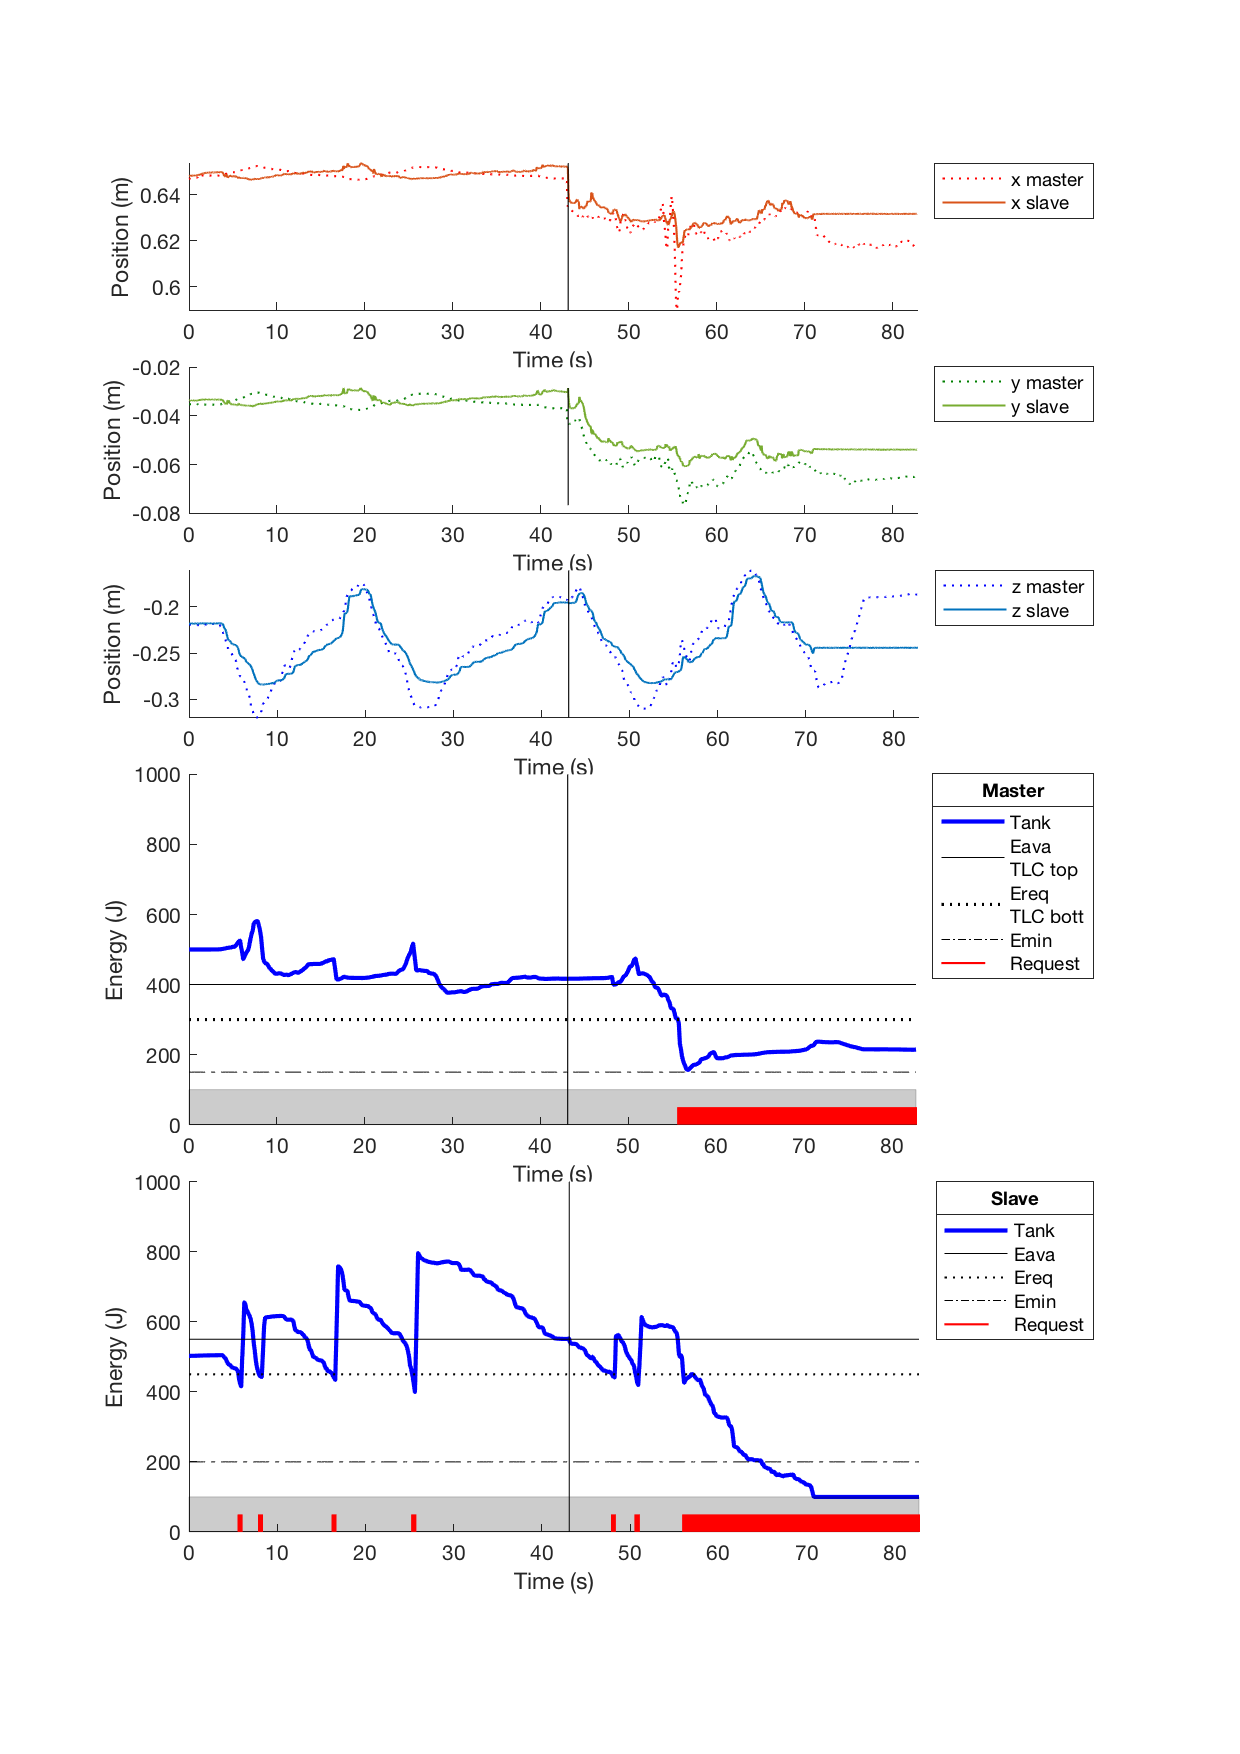
\includegraphics[width=\textwidth, keepaspectratio]{plots/pf90Delay/Position.pdf}
		\caption{Position tracking with 90° insertion approach. P-F control architecture with 0.2s RTT delay.}
		\label{graph:pf90Delay/Position}
	\end{figure}
\end{center}
\begin{center}
	\begin{figure}
		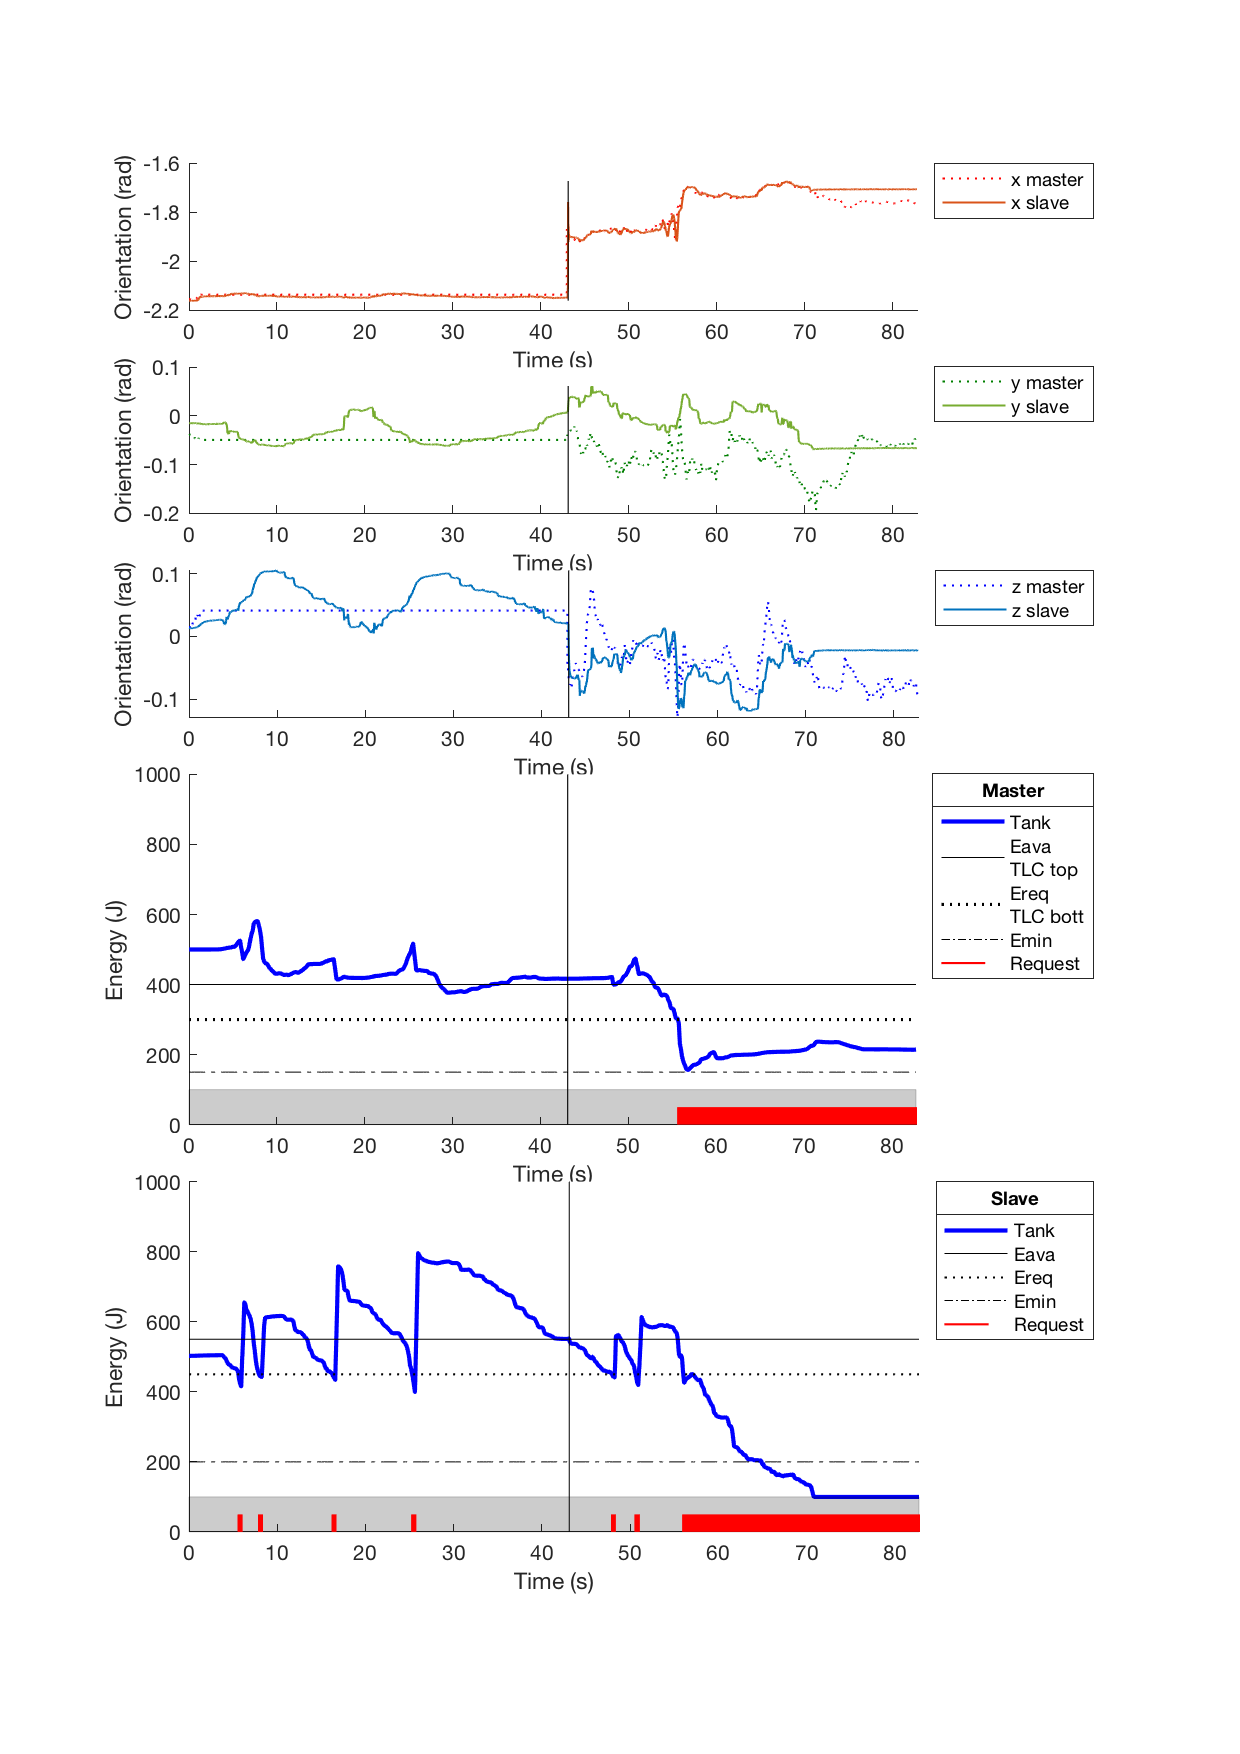
\includegraphics[width=\textwidth, keepaspectratio]{plots/pf90Delay/Orientation.pdf}
		\caption{Orientation tracking with 90° insertion approach. P-F control architecture with 0.2s RTT delay.}
		\label{graph:pf90Delay/Orientation}
	\end{figure}
\end{center}
\begin{center}
	\begin{figure}
		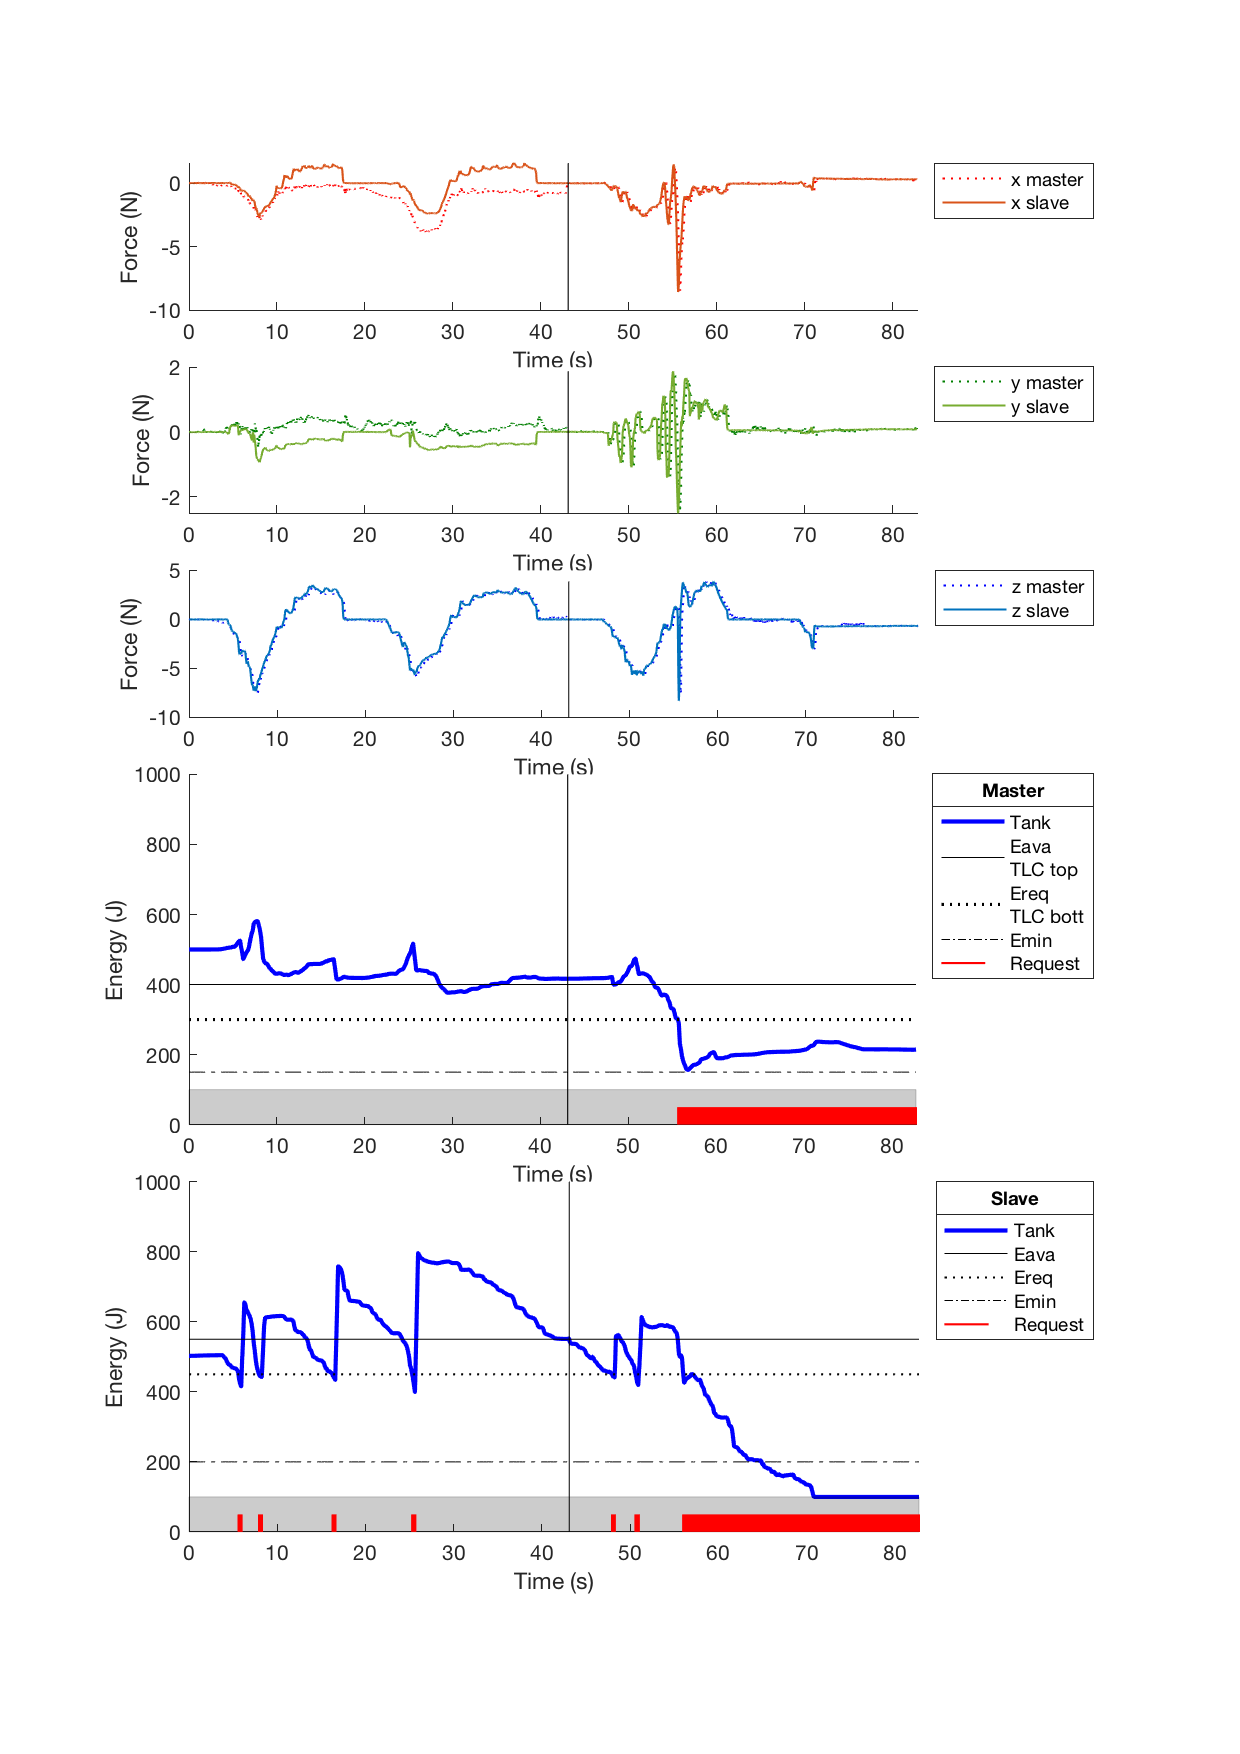
\includegraphics[width=\textwidth, keepaspectratio]{plots/pf90Delay/Force.pdf}
		\caption{Force tracking with 90° insertion approach. P-F control architecture with 0.2s RTT delay.}
		\label{graph:pf90Delay/Force}
	\end{figure}
\end{center}
\newpage
\subsubsection{Insertion with 45° approaching angle}\label{sec:insertion-with-45-approaching-angle}
In this test  (\figurename{ \ref{graph:pf45Delay/Position} to \ref{graph:pf45Delay/Force}}) the first two punctures have been done within the \textit{Pilot Mode}, and the other two with the standard controller.
The change of controller at time 50s is highlighted by a vertical line.\\
The instability in the second puncture causes energy draining in the whole system which is close to the passivity layer intervention. The instability is managed by the operator meaning that holds steadily the master manipulator dissipating the energy.
Thanks to the operator intervention the interaction forces are balanced by and the velocity at the end effector are not so high.
Without the operators reaction, the passivity layer would have intervened.
\begin{center}
	\begin{figure}
		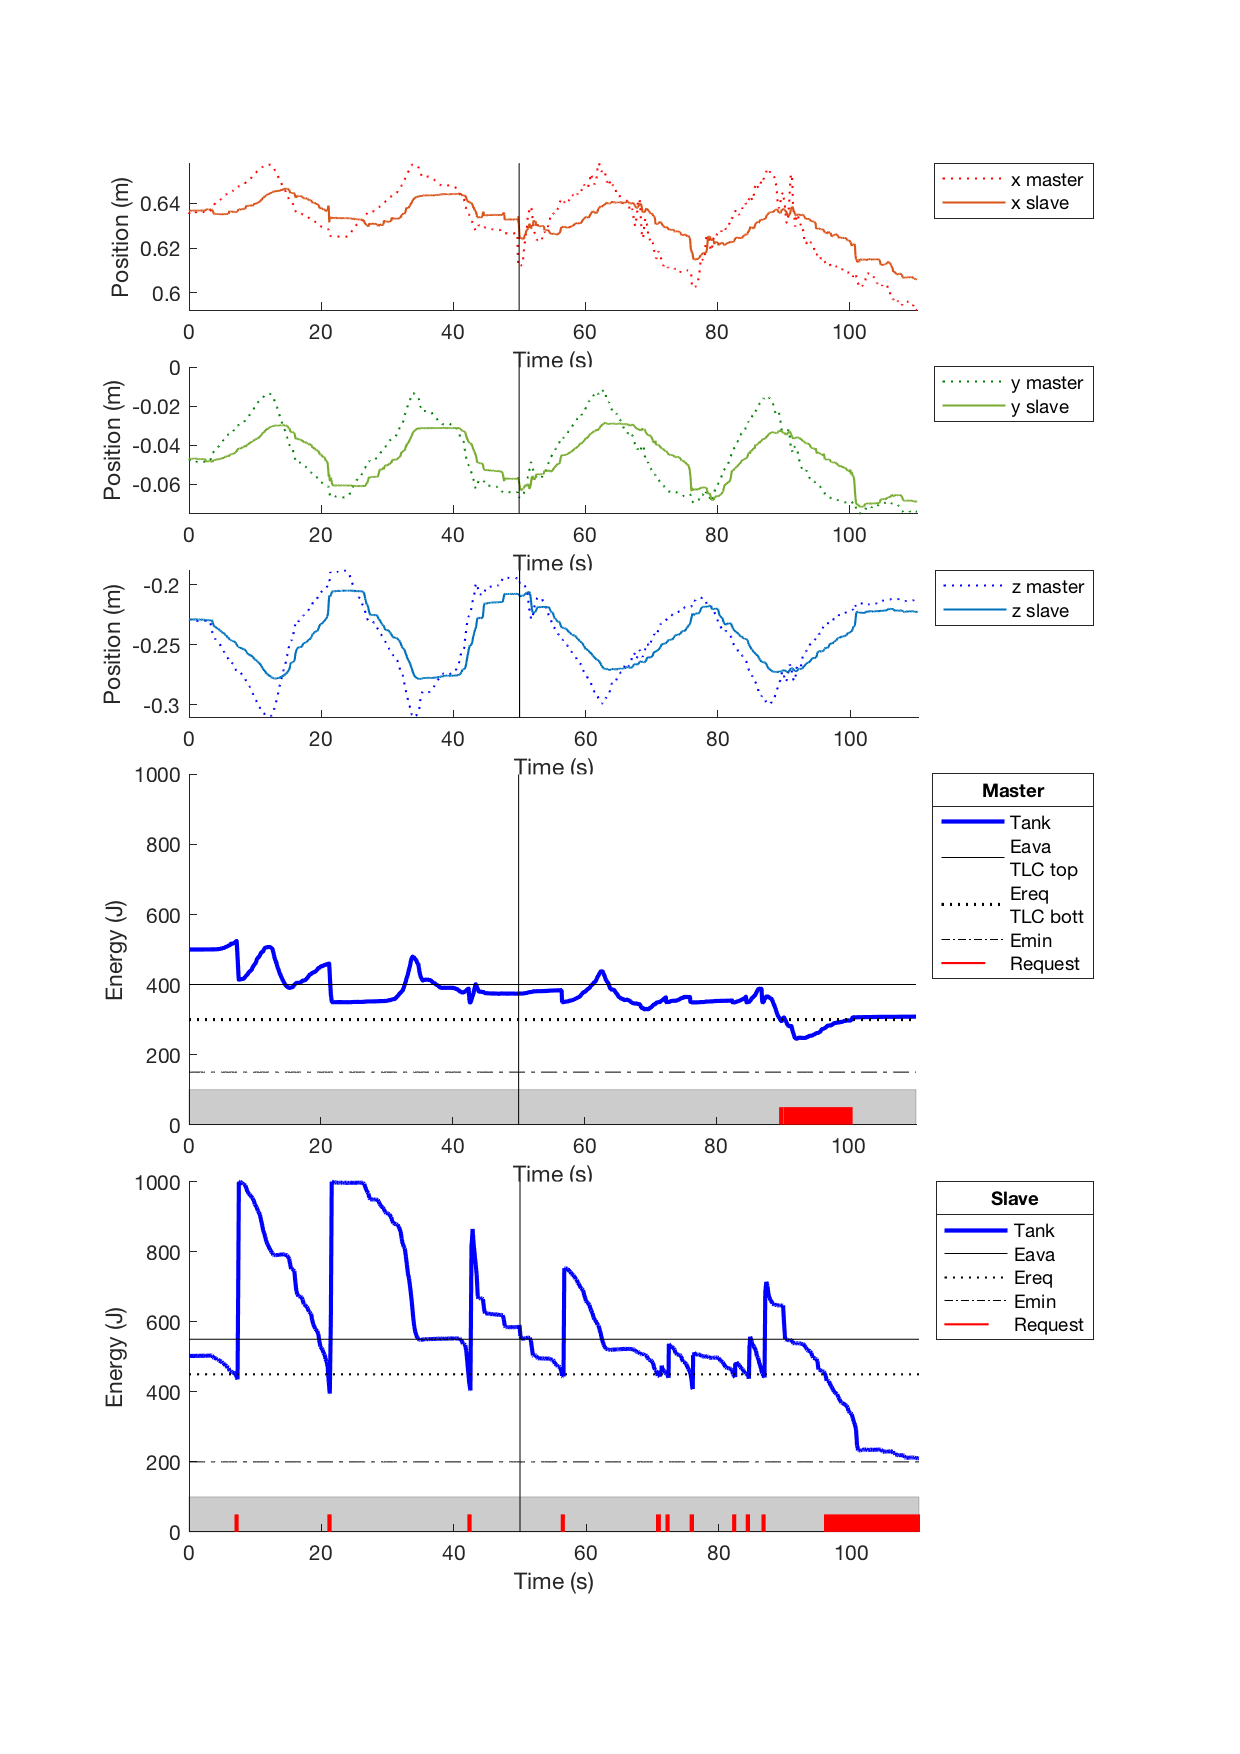
\includegraphics[width=\textwidth, keepaspectratio]{plots/pf45Delay/Position.pdf}
		\caption{Position tracking with 45° insertion approach. P-F control architecture with 0.2s RTT delay.}
		\label{graph:pf45Delay/Position}
	\end{figure}
\end{center}
\begin{center}
	\begin{figure}
		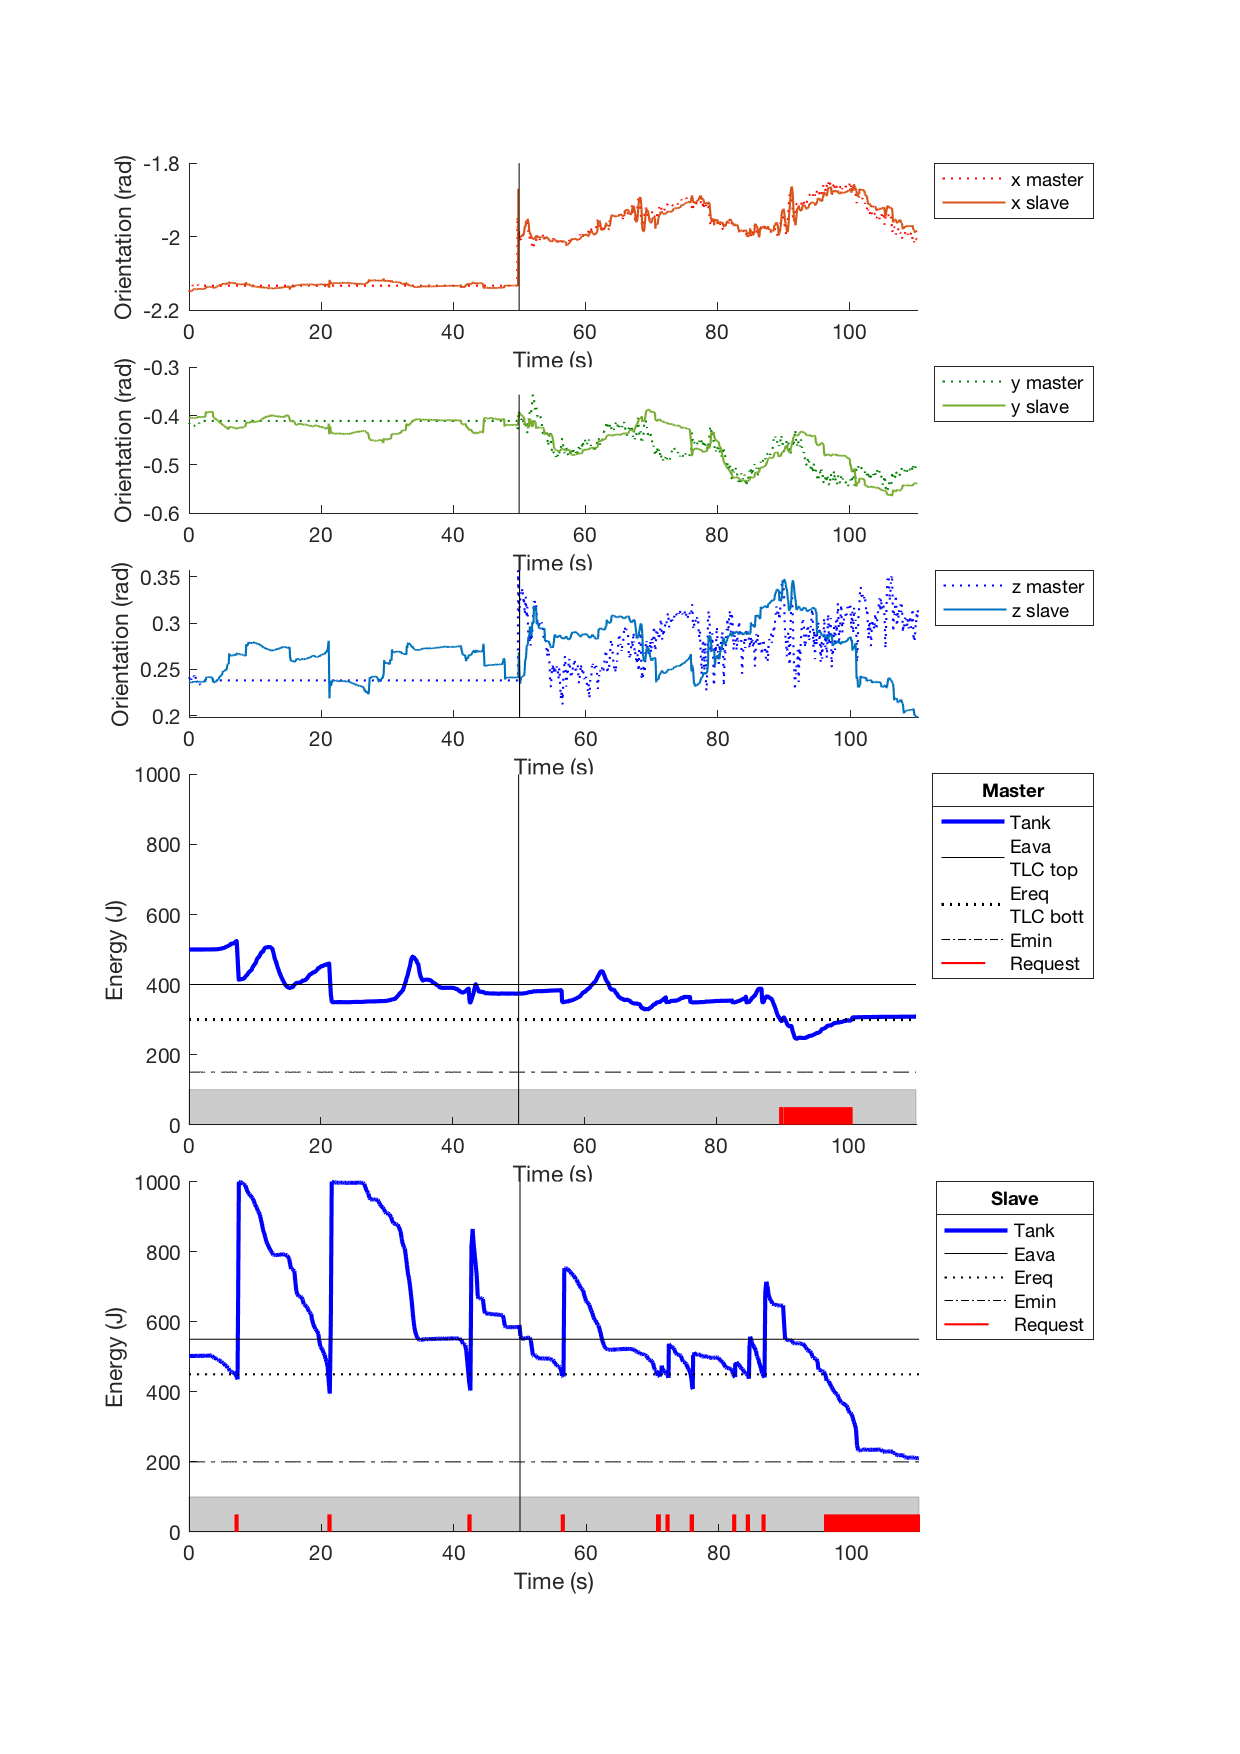
\includegraphics[width=\textwidth, keepaspectratio]{plots/pf45Delay/Orientation.pdf}
		\caption{Orientation tracking with 45° insertion approach. P-F control architecture with 0.2s RTT delay.}
		\label{graph:pf45Delay/Orientation}
	\end{figure}
\end{center}
\begin{center}
	\begin{figure}
		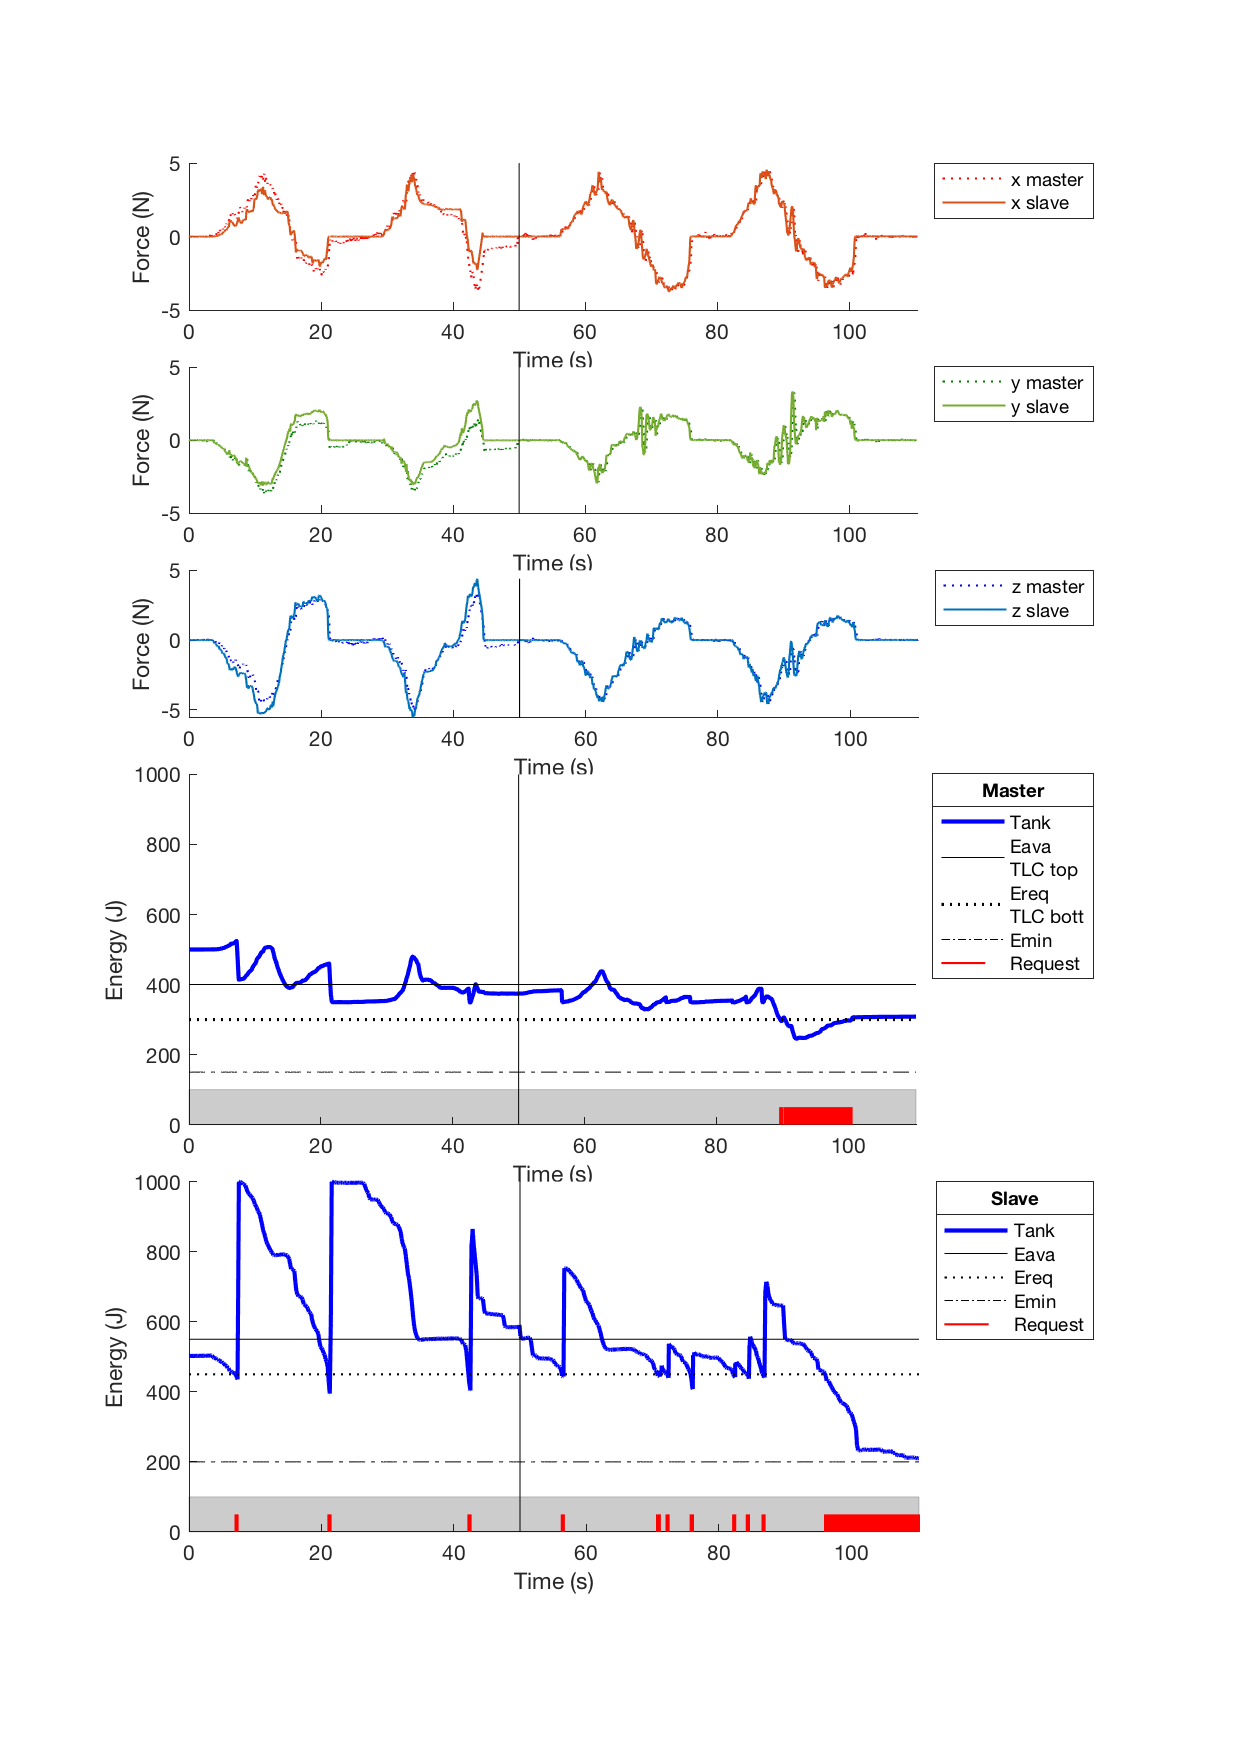
\includegraphics[width=\textwidth, keepaspectratio]{plots/pf45Delay/Force.pdf}
		\caption{Force tracking with 45° insertion approach. P-F control architecture with 0.2s RTT delay.}
		\label{graph:pf45Delay/Force}
	\end{figure}
\end{center}
\newpage

\section{Discussion}
The tuning of the Two-Layer has been kept as much as possible constant among all the experiments. Its not the preferred way to show the results because we can not show its best performance in each testing scenario, but we believe that with this choice can show the flexibility of the our system and better understand its limits with the purpose of enhance it in a near future.

The P-P architecture seems not to be the proper teleoperation architecture for the needle insertion procedure: 
\begin{itemize}
	\item The force feedback is estimated on the tracking error and is not due to the real interaction force.
This means that the operator feels an apparent inertia when controlling the end-effector due to the values of both $K_{p_{pos}}$ at master and slave sides.
	\item This inertia, if not to high, gives the feeling of handling the instrument, but when its effects become more prominent e.g. due to delays in the channel, it enhances the operators fatigue.
	\item A high perceived inertia negatively affects the level of transparency in the system by making less clear the difference between the free motion movement and the tissue insertion.
\end{itemize}

The P-F architecture is clearly the preferred architecture to address such procedure:
\begin{itemize}
	\item The force feedback is due to the real interaction force thus we can reach higher degrees of transparency.
	\item The lower stability of the P-F architecture is managed by the Two-Layer algorithm.
	\item When performing the insertion with the \textit{Pilot controller} we can also reach an high level of transparency by keeping the fundamental feedback along $z$.
\end{itemize}
Focusing on the Two-Layer framework we can also obtain better result if we tune it differently for each testing scenario.
We can made the following considerations on the basis of our experience while tuning the system:
\begin{itemize}
	\item To better manage the problem of delays we can act reducing the power rate. This helps because we can send less extra energy because of the RTT that the system needs to stop the energy flow.
	\item Between the two architectures the effects of energy leakage are different and more prominent in the P-P architecture. This suggest that a slight higher value for the Scale Factor is required for the P-P architecture. This will help in the procedures performed without the \textit{Pilot controller} in which the energy draining in the slave tank is due to a more prominent energy leaking, a side effect of our setup that does not allow the orientation feedback.
	\item The effects of instability and the corresponding intervention of the two layer are shown in the 90° insertion with delay with the P-F architecture (Section \ref{sec:insertion-with-90-approaching-angle}). Here the energy drops down both at master and slave side so that the system does not move any more.
	\item  The other example of instability, shown in the 45° insertion with delay with the P-F architecture  (Section \ref{sec:insertion-with-45-approaching-angle}), suggests that in the P-F architecture the \textit{passivity margin} of the system should be decreased.\\
	With a smaller passivity margin we would have seen the intervention of the passivity layer despite the dissipation due to the operator firmly holding the master console.
\end{itemize}	

%%%%%%%%%%%%%%%%%%%5

\clearpage
\thispagestyle{empty}